%\documentclass[10pt]{sig-alternate-05-2015}
%\documentclass[10pt,journal,compsoc]{IEEEtran}
%\documentclass[10pt, conference, letterpaper]{IEEEtran}
%\documentclass[10pt,journal,compsoc]{IEEEtran}
%\documentclass[letterpaper,twocolumn,10pt]{article}
%\usepackage{usenix,epsfig,endnotes}
%\documentclass[10pt, conference, letterpaper]{IEEEtran}
%\documentclass{sig-alternate-10pt}
%\IEEEoverridecommandlockouts
%\documentclass[preprint]{sigplanconf-eurosys}
\documentclass[nocopyrightspace]{sigplanconf-eurosys}

\usepackage{fancyhdr}
%\usepackage{algpseudocode}
\usepackage{graphicx}
\usepackage{epstopdf}
\usepackage{algorithm}
\usepackage{algorithmic}
\usepackage{multirow}
\usepackage{hhline}
\renewcommand{\algorithmicrequire}{\textbf{Input:}}
\renewcommand{\algorithmicensure}{\textbf{Output:}}
\renewcommand{\multirowsetup}{\centering}
\usepackage{setspace}


\usepackage{mathptmx}
\usepackage{helvet}
\usepackage{courier}
\usepackage{type1cm}

\usepackage{color}
\usepackage{amsmath}
\usepackage{url}
%\usepackage{hyperref}
%\usepackage{graphicx}
\usepackage{caption}

\usepackage{subcaption}
\usepackage{cases}
\usepackage{amsfonts}
\usepackage{colortbl}
%\usepackage[colorlinks,urlcolor=blue,dvipdfm]{hyperref}
\usepackage{hyperref}					% Reference
\hypersetup{colorlinks,%				% Reference color setup	
	linkcolor=blue,%
	citecolor=blue,
    urlcolor=blue,
	dvipdfm}
%\usepackage{cite}
\usepackage{flushend}
\usepackage{breakurl}
\usepackage{xspace}
\usepackage{enumitem}

\newtheorem{algorithm1}{Algorithm}
\newtheorem{theorem}{\noindent{\bf Theorem}}
\newtheorem{proposition}{\noindent{\bf Proposition}}
\newtheorem{constrain}{Constraint}
\newtheorem{definition}{Definition}
\newcommand{\TODO}[1]{\textcolor{red}{TODO: #1}}
\newcommand{\jc}[1]{{\footnotesize\color{blue}{[JC: #1]}}}
\newcommand{\fillme}{XXX\xspace}
\newcommand{\name}{BDS\xspace}
\newcommand{\company}{{Baidu}\xspace}
\newcommand{\Section}{\S}
%\usepackage[cmex10]{amsmath}
%\DeclareMathOperator{\E}{E}
%\hyphenation{recent op-tical net-works semi-conduc-tor}
%\tolerance=500
%\tolerance=1
%\emergencystretch=\maxdimen
\hyphenpenalty=5000
\tolerance=1000

\newcommand{\tightcaption}[1]{\vspace{-0.1cm}\caption{{\bf #1}}\vspace{-0.1cm}}
%\newcommand{\tightsection}[1]{\vspace{-0.02in}\section{#1}\vspace{-0.03cm}}
\newcommand{\tightsection}[1]{\section{#1}}
%\newcommand{\tightsubsection}[1]{\vspace{-0.02in}\subsection{#1}\vspace{-0.03cm}}
\newcommand{\tightsubsection}[1]{\subsection{#1}}
%\newcommand{\tightsubsection}[1]{\vspace{-0.02in}\subsection{#1}\vspace{-0.03cm}}
\newcommand{\tightsubsubsection}[1]{\vspace{-0.2cm}\subsubsection{#1}\vspace{-0.2cm}}

\newcommand{\mypara}[1]{\noindent{\bf {#1}:}~}
\newcommand{\myparatight}[1]{\noindent{\bf {#1}}~}
\newcommand{\myparaq}[1]{\noindent{\bf {#1}?}~}

\newcommand{\myparaittight}[1]{\noindent{\emph {#1}:}~}
\newcommand{\question}[1]{\noindent{\emph{Q:~#1}}\smallskip}
\newcommand{\myparaqtight}[1]{\noindent{\bf {#1}}~}


\newcounter{packednmbr}

\newenvironment{packedenumerate}{\begin{list}{\thepackednmbr.}{\usecounter{packednmbr}\setlength{\itemsep}{0.5pt}\addtolength{\labelwidth}{-4pt}\setlength{\leftmargin}{\labelwidth}\setlength{\listparindent}{\parindent}\setlength{\parsep}{1pt}\setlength{\topsep}{0pt}}}{\end{list}}

\newenvironment{packeditemize}{\begin{list}{$\bullet$}{\setlength{\itemsep}{0.5pt}\addtolength{\labelwidth}{-4pt}\setlength{\leftmargin}{\labelwidth}\setlength{\listparindent}{\parindent}\setlength{\parsep}{1pt}\setlength{\topsep}{0pt}}}{\end{list}}

\newenvironment{packedpackeditemize}{\begin{list}{$\bullet$}{\setlength{\itemsep}{0.5pt}\addtolength{\labelwidth}{-4pt}\setlength{\leftmargin}{\labelwidth}\setlength{\listparindent}{\parindent}\setlength{\parsep}{1pt}\setlength{\topsep}{0pt}}}{\end{list}}

\newenvironment{packedtrivlist}{\begin{list}{\setlength{\itemsep}{0.2pt}\addtolength{\labelwidth}{-4pt}\setlength{\leftmargin}{\labelwidth}\setlength{\listparindent}{\parindent}\setlength{\parsep}{1pt}\setlength{\topsep}{0pt}}}{\end{list}}

\newcounter{myfootnotecounter}
\newcommand\myfootnotemark{%
\addtocounter{footnote}{1}
\footnotemark[\thefootnote]
}
\newcommand\myfootnotetext[1]{%
\addtocounter{myfootnotecounter}{1}
\footnotetext[\value{myfootnotecounter}]{#1}
}
\newcommand\myfootnote[1]{%
\addtocounter{myfootnotecounter}{1}
\footnote{#1}
}

\begin{document}

\title{\name: A Centralized Near-Optimal Overlay Network for Inter-Datacenter Data Replication}

\authorinfo{
Yuchao Zhang$^1$,
Junchen Jiang$^2$,
Ke Xu$^3$,
Xiaohui Nie$^3$,\\
Martin J. Reed$^4$,
Haiyang Wang$^5$,
Guang Yao$^6$,
Miao Zhang$^6$,
Kai Chen$^1$,
\\
$^1$ HKUST 
$^2$ University of Chicago 
$^3$ Tsinghua University \\
$^4$ University of Essex 
$^5$ University of Minnesota at Duluth 
$^6$ Baidu \\
%
zyc@ust.hk, livejc@gmail.com, xuke@tsinghua.edu.cn, \\
nxh15@mails.tsinghua.edu.cn, mjreed@essex.ac.uk, haiyang@d.umn.edu, \\
\{yaoguang,zhangmiao02\}@baidu.com, kaichen@cse.ust.hk
}


\maketitle

%\begin{abstract}

Many important cloud services require replicating massive data from one datacenter (DC) to many DCs.
While recent efforts have greatly improved data transfers
between any pair of DCs, they are insufficient for bulk-data multicast,
because they do not harness server's capability to store-and-forward data as
well as abundant inter-DC overlay paths across geo-distributed DCs.
To exploit these opportunities, we present {\em \name},
an application-level multicast overlay network that
near-optimally sends inter-DC multicast traffic via
inter-DC overlay paths.
At its core, \name {} {\em fully centralizes} the overlay network control, allowing \name to maintain
an up-to-date global view of data delivery status in order
to fully utilize available overlay paths.
To handle network dynamics and workload churns,
\name decouples the centralized control algorithm
into overlay routing and transfer scheduling, each of which
can be solved efficiently.
This enables \name to  update overlay routing
decisions frequently  (e.g.,
every other second)
at the scale of multicasting hundreds of TB
data over tens of thousands overlay paths.
A pilot deployment in one of the largest online
service providers shows that \name achieves 3-5$\times$
speedup over the provider's existing system and several widely used overlay routing systems.

%Many important cloud services require replicating massive
%amounts of data from one datacenter (DC) to many DCs.
%While recent work has focused on improving the WAN performance
%between any pair of DCs, it is necessarily incomplete,
%as it falls short of
%harness servers' capability to store-and-forward data, as
%well as inter-DC overlay paths available in abundance
%in globally deployed DCs.
%To explore these unexplored opportunities, we present {\em \name},
%an application-level multicast overlay network that
%near-optimally sends inter-DC multicast traffic via
%inter-DC overlay paths.
%At its core, \name {} {\em fully centralizes} the
%control of the overlay network, allowing \name to maintain
%an up-to-date global view of data delivery status in order
%to fully utilize the available overlay paths.
%To handle dynamic network conditions and workload churns,
%\name decouples the centralized control algorithm
%into overlay routing and transfer scheduling, each of which
%could be solved efficiently.
%This enables \name to  update overlay routing
%decisions frequently  (e.g.,
%every other second)
%at scales of multicasting hundreds of TB
%data over $10^4$s of potential overlay paths.
%A pilot deployment in one of the largest online
%service providers shows that \name achieves 3-5$\times$
%speedup over the provider's existing systems, as well
%as several widely used overlay routing systems.

%For large-scale online service providers, one of the most
%common communication patterns of inter-datacenter (DC)
%workload is {\em bulk-data inter-DC multicast}:
%replicating bulk data from one DC to multiple DCs.
%While recent work has sought to improve bulk-data
%transfers by optimizing WAN performance, it is necessarily
%incomplete, as it falls short of fully exploring servers'
%capability to store-and-forward data, as well as
%the disjoint inter-DC paths existing in abundance.
%%Inspired by the early success of multicast overlay networks,
%Instead, we argue that an optimal application-level multicast
%overlay network is needed to utilize these unexplored
%opportunities by dynamically scheduling and routing inter-DC
%data transfers via overlay paths.
%Despite these promises, building an optimal overlay network
%for inter-DC multicast poses two challenges:
%(1) the sheer amounts of servers and overlay paths
%render it untenable to select optimal overlay paths
%in real-time, and (2) it must prevent delay of
%latency-sensitive traffic caused by bulk-data multicasts on
%any multicast overlay paths.
%We present {\em \name}, a simple yet near-optimal overlay network
%for bulk-data inter-DC multicasts.
%Contrary to the intuition that servers must retain the capability
%to adapt locally (and thus suboptimally)
%in order to scale out, \name demonstrates the
%feasibility and practical benefits of fully centralizing the
%control of the overlay network.
%The key insight underlying this centralized design is the
%observation that bulk-data transfers tend to last on coarse
%timescales so they can
%tolerate a slight delay of centralized decision-making
%in the hope of getting
%a closer-to-optimal overlay routing.
%Moreover, centralized bandwidth allocation on the granularity
%of each data transfer proves efficient in eliminating
%interference of bulk-data transfers on latency-sensitive traffic.
%%\name is built on design choices:
%%(a) fully centralized decision-making in near real-time, and
%%(b) enforcing a clean, dynamic separation of bandwidth.
%%While both design choices introduce costs on performance
%%(\name is unable to update decisions in real time or achieve
%%full link utilization), we believe these costs are outweighed by
%%the benefits, such as centralized optimization driven by a global
%%view.
%A pilot deployment of \name in one of the largest online
%service providers shows that \name achieves 3-5$\times$
%speedup over the provider's existing systems, as well
%as several widely used overlay routing systems.


%Distributing bulk data across datacenters (DCs) in a timely and
%cost-effective manner is critical to large-scale online service
%providers.
%While recent research has significantly improved the WAN performance
%between DCs, we argue that a multicast overlay network that optimally
%schedules and delivers data in a way that fully exploits available
%overlay paths is essential to achieving desirable performance.
%Drawing on the experience of a large online service providers, we
%observe two requirements of an inter-DC multicast overlay network:
%(1) overlay routing and scheduling needs to be driven by an
%up-to-date global view of data delivery status at all servers, and
%(2) it must prevent delay of latency-sensitive
%traffic caused by bulk data transfers.
%
%This paper presents \name, a near-optimal inter-DC multicast overlay
%network that distributing bulk data.
%At the core of \name are two design choices.
%First, decision making in \name is fully centralized; the \name
%controller directly orchestrates servers to split, reorder, and
%deliver data dynamically along overlay paths, in order to
%circumvent inter-/intra-DC bottlenecks.
%Second, \name enforces a dynamic separation of bandwidth allocated
%for bulk data transfers and latency-sensitive traffic.
%While both design choices introduce costs in performance (i.e.,
%\name is unable to update decisions in real time or achieve full
%link utilization), our design philosophy is that these costs are
%outweighed by the benefits of centralized optimization driven
%by a global view.
%Using a pilot deployment of \name in one of the largest search
%engine service providers, we show that \name achieves 3-5$\times$
%speedup over the provider's existing systems and the techniques
%widely used in today's content delivery networks.


%Drawing on lessons from the decade-long evolution of similar systems in Baidu,
%\name take a centralized approach, which uses a controller to maintains the
%data delivery status in all servers, and update the scheduling and overlay routing
%decisions in near real time by solving a multicommodity flow problem using a
%near-optimal yet efficient algorithm.
%The key insight underlying \name's centralized architecture is the observation that
%the cost of not being able to adapt to network conditions in real time (such as in
%a decentralized system) is greatly outweighed by the benefits of centralized
%control to optimally update overlay routing and scheduling even at a coarse
%timescale (every few seconds), as well as the resulting system that has less
%complexity.

\end{abstract}

\begin{abstract}

Many important cloud services require replicating massive data from 
one datacenter (DC) to multiple DCs. While the performance of pair-wise 
inter-DC data transfers has been much improved, prior solutions
are insufficient to optimize bulk-data multicast, as they fail to 
explore the capability of servers to store-and-forward data, as well as 
the rich inter-DC overlay paths that exist in geo-distributed DCs.
To take advantage of these opportunities, we present {\em \name}, an 
application-level multicast overlay network for large-scale inter-DC data replication. At the core of \name is a {\em fully centralized} 
architecture, allowing a central controller to maintain an up-to-date
global view of data delivery status of intermediate servers, in 
order to fully utilize the available overlay paths. To quickly react 
to network dynamics and workload churns, \name speeds up the control 
algorithm by decoupling it into selection of overlay paths and
scheduling of data transfers, each can be optimized efficiently. This
enables \name to update overlay routing decisions in near real-time 
(e.g., every other second) at the scale of multicasting hundreds of TB
data over tens of thousands of overlay paths. A pilot deployment in 
one of the largest online service providers shows that \name can 
achieve 3-5$\times$ speedup over the provider's existing system and 
several well-known overlay routing baselines. 

\end{abstract}


\section{Introduction}

For large-scale online services, such as Google, Facebook, and
Baidu, an important inter-datacenter (inter-DC) communication pattern is
{\em inter-DC bulk-data multicast}--replicating massive amounts of data
(e.g., user logs, search engine indexes, offline file sharing,
forum posts, and databases)
from one DC to many geo-distributed DCs.
%A common inter-DC communication pattern {\em bulk-data inter-DC multicast},
%which replicates data (e.g., user
%logs, search engine indexes, offline file sharing, forum posts, and
%databases) from one DC to any set of destination DCs.
Our study on the workload of
\company reveals that
inter-DC multicast amounts to 91\% of inter-DC traffic
(\Section\ref{sec:motivation}), which corroborates the findings of
other large-scale online service providers~\cite{kumar2015bwe,zhang2016piebridge}.
As data sizes continue to explode and more DCs are deployed
globally, inter-DC data transfers are expected
to grow significantly, which is a key driving force behind
recent efforts towards improving inter-DC data transfer~\cite{savage1999Theend,jain2013b4,kumar2015bwe,hong2013achieving,zhang2015guarantee}.


%Global-scale online services, such as Google, Facebook, and Baidu,
%depend crucially on the ability to distribute data across
%geo-distributed datacenters (DCs) in a timely and cost-effective
%manner. This has introduced substantial challenges, as data sizes
%continue to explode and more DCs are deployed to reach a global
%footprint.
%These trends have been a key driving force behind recent efforts
%to optimize the WAN performance between two
%DCs~\cite{b4,bwe,swan,??,??,??}.


\begin{figure}[t!]
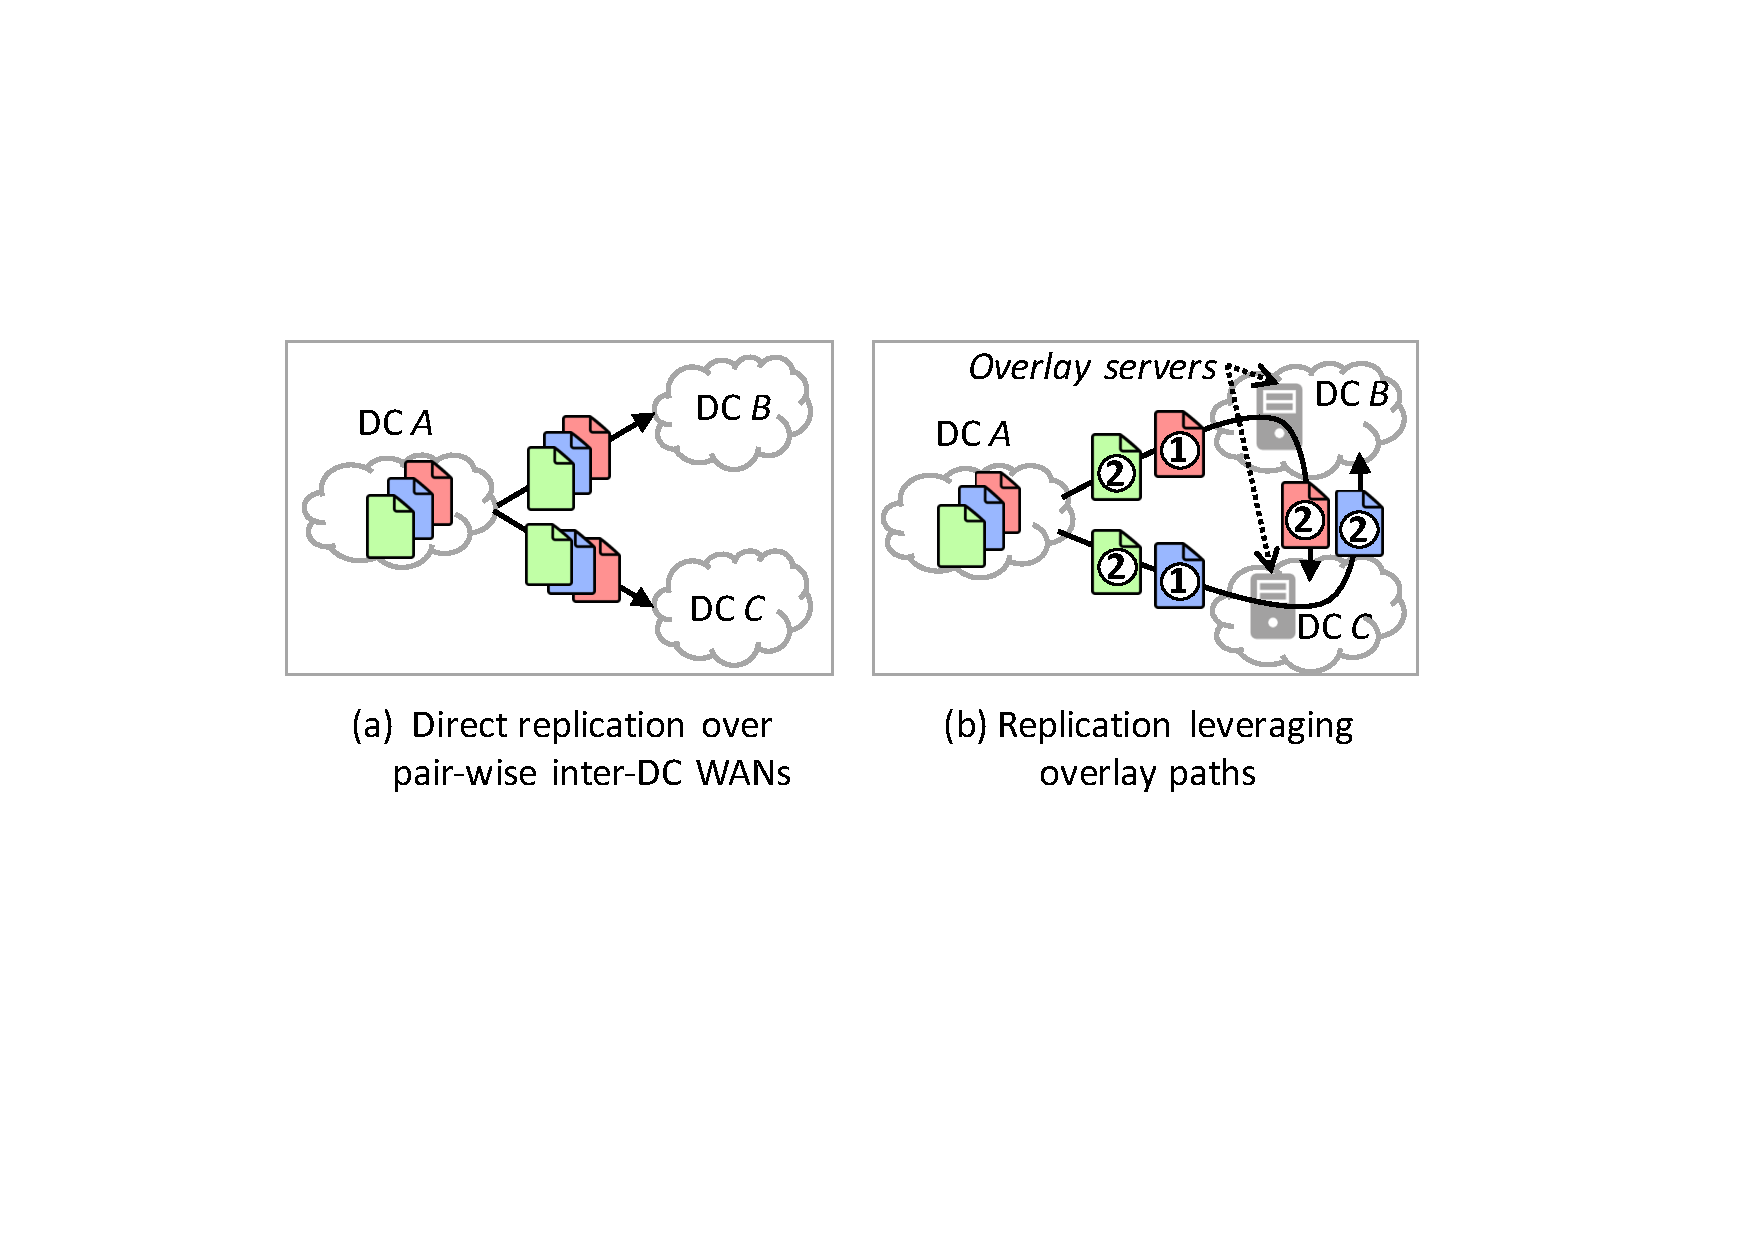
\includegraphics[width=83mm]{images/intro-example-3.pdf}
\vspace{-0.4cm}
\tightcaption{A simple network topology illustrating how
overlay paths reduce inter-DC multicast completion time.
%Assume the bottleneck is the outgoing router of DC $A$.
Assume that each DC has 1GB/s one-directional WAN links to any other
DC, and that $A$ wants to send 3GB data to $B$ and $C$.
Sending data from $A$ to $B$ and $C$ separately
takes 3 seconds (a),
but using overlay paths $A$$\rightarrow$$B$$\rightarrow$$C$
and $A\rightarrow$$C$$\rightarrow$$B$
simultaneously takes only 2 seconds (b).
The circled numbers show the order for each data piece
 is sent. }
\label{fig:intro}
\vspace{-0.4cm}
\end{figure}

Prior efforts to optimize inter-DC data replication have focused on improving the wide area network (WAN) performance between any pair of DCs. These WAN-centric approaches, however, are imcomplete, as they fail to leverage the application-level overlay paths available in
geo-distributed DCs, or server's capability to
store-and-forward data.
As illustrated in Figure~\ref{fig:intro}, the performance of
inter-DC multicast could be substantially improved by
delivering data in parallel via multiple overlay servers
acting as intermediate points to circumvent slow WAN paths and
performance bottlenecks in DC networks.
%(More examples can be found in \Section\ref{sec:motivation}.)
Note that these overlay paths must be {\em bottleneck-disjoint} (i.e., they do
not share common bottleneck links, e.g., $A$$\rightarrow$$B$$\rightarrow$$C$,
$A$$\rightarrow$$C$$\rightarrow$$B$ in Figure~\ref{fig:intro}), and that
such bottleneck-disjoint overlay paths are available in abundance in
geo-distributed DCs.




This paper presents {\em \name}, an {\em application-level
multicast overlay network}, which splits data into fine-grained
units and sends them in parallel via bottleneck-disjoint
overlay paths. These paths are selected dynamically in response to changes in
network conditions and the up-to-date data delivery status on each server.
%sends them in parallel on selectively picked
%overlay paths, and dynamically adapts the overlay routes and
%schedules in response to changes in network conditions and
%workload churns.
Note that \name selects application-level overlay paths and is thus
complementary to network-layer techniques that
optimize the WAN performance.
While application-level multicast overlays have been applied
in other contexts
(e.g.,~\cite{Liebeherr2002Application,Wang2007mTreebone,
Andreev2013Designing,Mokhtarian2015Minimum}), building one
for large online service providers poses two
challenges.
%Building on the operational experience of
%\company\footnote{Anonymized for double-blind reviewing},
%a large online service providers, we summarize two challenges,
%which to our best knowledge do not have direct solution.
First, as each DC has tens of thousands of servers, the
resulting sheer amount of overlay paths makes it
unwieldy to update overlay routing decisions in real time.
Prior work where servers make local reactive decisions~\cite{kostic2003bullet,Repantis2010Scaling,Huang2014A} cannot result in optimal scheduling due to the invisibility of global information, and the improved solution that prunes the set of overlay paths is limited by strictly structured (e.g., layered) topologies~\cite{Nygren2010The}, so we cannot simply borrow techniques from these works.
%The performance could be suboptimal by simply borrowing techniques
%from prior work, such as servers making local reactive
%decisions~\cite{kostic2003bullet,Repantis2010Scaling,Huang2014A},
%or pruning the set of overlay paths by strictly
%structured (e.g., layered) topologies~\cite{Nygren2010The}.
Second, even a small increase in the delay of latency-sensitive traffic
can cause significant revenue loss, so the bandwidth usage
of inter-DC bulk-data multicasts must be tightly controlled
to avoid negative impact on latency-sensitive
traffic\myfootnote{Despite priority-based queuing
at each DC border router, bulk-data multicasts compete
inter-DC WAN (not managed by \company) with
latency-sensitive traffic, leading to negative impacts on
latency-sensitive traffic.}.
%, even at the expense of a slightly lower link utilization.

%Inspired by the multicast overlay networks, we argue that to optimize bulk-data multicast,
%a similar {\em application-level multicast
%overlay network} is needed to optimally deliver data in a way that
%fully utilizes inter-DC overlay paths.
%To replicate a data file from one DC to multiple DCs, this overlay
%multicast network will send different parts of the data
%simultaneously along selectively picked overlay paths, and
%dynamically adapt the overlay routing in response to changes in
%network conditions and resource availability.




%we argue that an {\em inter-DC multicast
%overlay} network that optimally schedules and routes data via
%overlay paths is essential to ensuring the desirable performance
%for two reasons.
%First, the need for multicasting data to a subset of (or all) DCs
%is endemic in online service providers; e.g.,
%Google has seen a \fillme-fold increase in \fillme years
%in the amount of data that needs to be distributed to all
%DCs~\cite{??}, and this number would only multiply with more
%DCs deployed.
%Second, the improved WAN performance between any DC pair can be
%fully utilized only when used with an inter-DC multicast overlay
%network that
%splits data in fine granularities and optimally select
%overlay paths to circumvent inter-/intra-DC bottlenecks.



%%While these efforts have shown promising improvement on the performance of pairwise
%%inter-DC WANs, we argue that an efficient multicast overlay network that optimally
%%schedules and routes data from each DC to multiple DCs via inter-DC overlay paths
%%is essential to ensuring desirable performance and fully utilizing the improved
%%pairwise inter-DC data transfer.
%While multicast overlay networks have been studied extensively
%in settings of peer-to-peer (P2P) streaming~\cite{??,??} and
%content delivery networks (CDNs)~\cite{??,??}, it remains unclear
%whether existing approaches apply to the scale of large online
%service providers like Google and Baidu.
%%The conventional wisdom has been that to operate at scale and react
%%in real time, one has to either organize overlay nodes in a
%%strictly structured (and thus suboptimal) topology
%%(e.g.,~\cite{akamai}), or use a hybrid (and thus more
%%complex) control mechanism (e.g.,~\cite{vdn}) with a local
%%logic adapting in real time and a global logic updating every
%%few minutes.
%Drawing on the operational experience from
%\company\footnote{Anonymized for double-blind reviewing}, a large
%online service providers, we see two key requirements
%of an inter-DC multicast overlay network.
%First, because these DCs have more servers and thus
%exponentially more overlay paths than CDNs or P2Ps,
%it is untenable to exploit all overlay paths by
%traditional approaches, such as decentralized or hybrid path
%selection (e.g.,~\cite{??,??}), or structured topologies
%(e.g.,~\cite{akamai}).
%Second, these WANs are shared by latency-sensitive traffic
%and bulk background traffic.
%Because any small increase in delay of
%latency-sensitive traffic can cause substantial revenue losses,
%there is a strong need to prevent interference on
%latency-sensitive traffic, even at the expense of slightly lower
%link utilization.


%while a more decentralized overlay network protocol
%is conceptually simpler, it is untenable for them to fully
%utilize the overlay paths, so we see a great room for
%improvement, especially at tail performance. This motivates
%the fully centralized architecture that maintains a fresh
%global view for decision making.
%Second, adding even a small delay in latency-sensitive data
%can cause significant revenue losses. Therefore, it is
%acceptable to enforce a clean bandwidth separation between
%bulk traffic delivery and latency-sensitive data, even at
%the cost of lower link utilization.
%
%But designing a multicast overlay for DCs of online service
%providers is different in two key aspects.
%First, these DCs have more servers in DCs, and much more overlay
%paths, so it is necessary to maintain an up-to-date global view
%of data delivery status on all servers to fully exploit these
%paths.
%Second, the WANs are shared by latency-sensitive user data and
%background bulk data, creating a need for minimizing the data
%distribution latency while preventing negative
%impacts on the latency-sensitive data.

To address these challenges, \name fully {\em centralizes}
the scheduling and routing of inter-DC multicast.
Contrary to the intuition that servers must retain certain
local decision-making capability to achieve scalability and
responsiveness to performance events, \name's centralized design
is built on two empirical observations (\Section\ref{sec:overview}).
(1) While it is less likely to make
centralized decisions in real time, most multicast data transfers
last for tens of seconds and thus can tolerate certain commutation delay with
the central controller in exchange for optimal routing and scheduling based on a global view.
(b) Centrally coordinated bandwidth allocation is amenable
to minimizing the interference between inter-DC multicast
traffic and latency-sensitive traffic.% by enforcing bandwidth allocation on overlay paths.
%(c) Finally, a centralized design is amenable to a simple
%implementation from an engineering perspective;
%e.g., the program running locally on the server side is
%only triggered by data arrivals or control messages, and
%thus can be largely stateless.

%This paper presents {\em \name}, a near-optimal multicast
%overlay network for inter-DC bulk data multicast.
%At the core of \name is the decision of {\em fully centralizing
%the scheduling and routing of bulk-data multicast}.
%%This paper presents {\em \name}, a near-optimal inter-DC multicast
%%overlay network, which minimizes data distribution delay from one
%%DC to any subset DCs by dynamically splitting,
%%reordering, and deliver data via overlay paths selected
%%from all server-level paths between the source DC and destination DCs.
%%\name focuses on distributing background bulk data (e.g., \fillme),
%%which is by several orders of magnitudes larger than
%%latency-sensitive user data.
%Contrary to the intuition that, in order to scale out
%and be responsive, servers must retain the capability to make
%certain local decisions, \name's centralized design
%is built on the several empirical observations:
%\begin{packeditemize}
%\item First, while it is indeed impractical to update centralized
%decision-making in real-time, bulk-data transfers, which take
%at least tens of seconds, can tolerate a small update delay in
%overlay routing decisions
%in the hope of getting closer-to-optimal decisions based on
%a global view of data delivery status.
%\item Second, centrally coordinated decision-making makes it easier
%to enforce bandwidth allocation on all overlay paths,
%and thus eliminate interference of bulk-data
%transfers on latency-sensitive traffic.
%\item Finally, a centralized design is amenable to a simple
%implementation from an engineering perspective;
%e.g., the program running locally on the server side is
%only triggered by data arrivals or control messages, and
%thus can be largely stateless.
%\end{packeditemize}


The key to realizing benefits of \name's centralized design in practice is to update
the overlay network on the timescale of seconds in response to dynamic network conditions
and failures. \name achieves this by {\em decoupling} its centralized control
into two optimization problems, scheduling of data transfers, and
overlay routing of individual data transfers.
This decoupling attains provable optimality, and at the same time,
allows \name to update overlay network routing and scheduling in
a fraction of second (four orders of magnitude faster than solving
routing and scheduling) jointly on workloads
of a large online service provider (e.g., sending $10^5$s of data blocks
simultaneously along $10^4$s of disjoint overlay paths, and updating
the routing every other second).


%At the core of \name are two design choices.
%\begin{packeditemize}
%\item {\em Centralized decision-making:}
%Decision making in \name is fully centralized; the \name
%controller maintains a global view of data delivery status on
%all servers
%and makes overlay routing and scheduling decisions every
%few seconds (by default, 3 seconds).
%\name solves a multicommodity problem using
%a near-optimal algorithm amenable to efficient incremental
%updates.
%\item {\em Clean bandwidth separation:}
%To prevent delay caused by background data on
%latency-sensitive user data, \name monitors the
%aggregated traffic volume
%of latency-sensitive data, and maintains a clean, dynamic
%bandwidth
%separation by enforcing the maximum amount of bulk-data
%multicast sent from each server.
%\end{packeditemize}

%While \name's design choices introduce performance costs (i.e.,
%\name does not update decisions in real time or achieve full
%link utilization), our design philosophy is that these costs are
%favorably outweighed by several benefits.
%% of near-optimal global optimization
%%as well as the resulting simpler solution from an engineering
%%perspective.
%%This observation inspired the key insight underlying \name that
%%multicasting bulk data can tolerate a small amount of delay in
%%exchange for closer-to-optimal decisions overlay routing and
%%scheduling.
%(1) Since delivering bulk data takes tens of seconds to
%minutes, \name can tolerate a delay of updating centralized
%control decisions at coarse timescales of several
%seconds in exchange for closer-to-optimal decisions made by
%the centralized controller.
%(2) The observation that the aggregation of
%latency-sensitive traffic tends to
%be stable on timescales of several seconds suggests that it is
%plausible to eliminate undesired interference on
%latency-sensitive traffic by clean bandwidth separation
%while achieving a high link utilization.
%%Moreover, having a global view on the delivery status of all objects in all
%%servers allows the controller to remarkably improve overlay routing and
%%scheduling decisions, which would be impossible otherwise.
%(3) Finally, these design choices are amenable to a simple
%implementation from an engineering perspective;
%e.g., the program running locally on the server side is
%only triggered by data arrivals or control messages, and
%thus can be largely stateless.


We have implemented a prototype of \name and integrated it in
\company, one of the largest search service providers.
We deployed \name in 10 DCs and ran a pilot study on 500~TB
data for over 7 days (70~TB per day).
Our real-world experiments show that \name achieves 3-5$\times$
speedup over \company's existing solution, and it can eliminate almost all the
incidents of excessive bandwidth consumption by bulk-data
transfers.
Using real trace-driven evaluation and microbanchmarking,
we also show that \name outperforms techniques widely used in
CDNs, and that \name can handle the workload of \company's
inter-DC multicast traffic with one general-purpose server.
We also show that \name can tolerate various failure scenarios.


Our contributions are summarized as following:
\begin{packeditemize}
\item Characterizing the workload of inter-DC bulk-data
replication to motivate the need of application-level
multicast overlay networks (\Section\ref{sec:motivation}).
\item Presenting \name, an application-level
multicast overlay network that achieves near-optimal flow completion
time with a centralized control scheme (\Section\ref{sec:overview},\ref{sec:logic},\ref{sec:system}).
\item Demonstrating the practical benefits of \name by a real-world
 deployment in a large online service provider (\Section\ref{sec:evaluation}).
\end{packeditemize}


%\section{A case for application-level inter-DC multicast overlays}
\label{sec:motivation}

We start by providing a case for an application-level multicast
overlay network. We first characterize the inter-DC multicast
workload in \company, a global-scale online service provider
(\Section\ref{subsec:motivation:multicast-traffic}). We then show
the opportunities of improving multicast performance by leveraging
disjoint application-level overlay paths available in geo-distributed
DCs (\Section\ref{subsec:motivation:case-for}). Finally, we examine
\company's current solution of inter-DC multicast (\alg), and draw
lessons from real-world incidents to inform the design of \name
(\Section\ref{subsec:motivation:baseline}). The findings are based on
a dataset of \company's inter-DC traffic collected in a duration of
seven days. The dataset comprises of about 1265 multicast transfers
among 30+ geo-distributed DCs.


\subsection{\company's inter-DC multicast workload}
\label{subsec:motivation:multicast-traffic}


\begin{table}[t!]
\begin{center}
\resizebox{3in}{!}{
%\begin{tabular}{p{2cm}<{\centering}|p{2cm}<{\centering}}
\begin{tabular}{| c | c|}
\hline
 \rowcolor[gray]{0.9}
\textbf{Type of application} & \textbf{\% of multicast traffic} \\
\hline\hline
All applications & 91.13\%~\myfootnotemark\\
\hline
Blog articles & 91.0\% \\% 4648.92 vs 41372.56 in GB
\hline
Search indexing & 89.2\%\\% 16766.7 vs 138418.12
%\hline
%International & 98.15\%\\% 1297.7 vs 68699.97
\hline
Offline file sharing & 98.18\%\\% 2792.4 vs 150234.25
%\hline
%Scholar & 98.09\%\\% 451.22 vs 23134.21
\hline
Forum posts & 98.08\%\\% 964.62 vs 49327.01
\hline
Other DB sync-ups & 99.1\%\\% ?? vs ??
\hline
\end{tabular}
}
\end{center}
\caption{Inter-DC multicast (replicating data from
one DC to many DCs) dominantes \company's inter-DC
traffic.}
%\vspace{-0.2cm}
\label{table:rate}
\end{table}
\myfootnotetext{The overall multicast traffic share is estimated using the traffic that goes through one randomly sampled DC, because we do not have access to information of all inter-DC traffic, but this number is consistent with what we observe from other DCs.}

\mypara{Share of inter-DC multicast traffic}
Table~\ref{table:rate} shows inter-DC multicast (replicating data
from one DC to multiple DCs) as a fraction of all inter-DC traffic.
We see that inter-DC multicast dominates \company's overall inter-DC
traffic (91.13\%), as well as the traffic of individual application
types (89.2 to 99.1\%). The fact that inter-DC multicast traffic
amounts to a dominating share of inter-DC traffic highlights {\em the
importance of optimizing the performance of inter-DC multicast.}

\begin{figure}[t]
        \centering
        \begin{subfigure}[b]{0.23\textwidth}
                \centering
                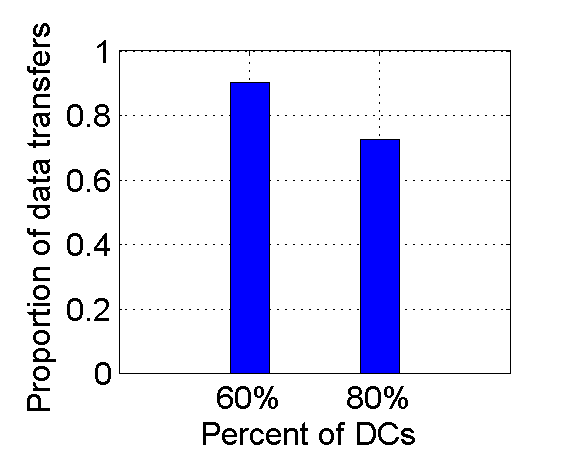
\includegraphics[width=\textwidth]{images/destinationDC_v2.eps}%NeedMulticast.m
                \caption{Proportion of multicast transfers destined to percent of DCs.}
                \label{fig:bulk:dest}
        \end{subfigure}
	\hspace{0.1cm}
        \begin{subfigure}[b]{0.23\textwidth}
                \centering
                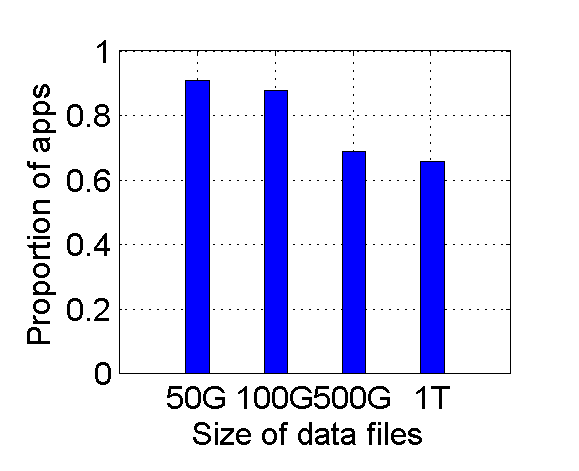
\includegraphics[width=\textwidth]{images/DataSize_v2.eps}
                \caption{Proportion of multicast transfers larger than certain threshold.}
                \label{fig:bulk:size}
        \end{subfigure}
        \vspace{-0.4cm}
        \tightcaption{Inter-DC multicasts (a) are destined to a significant
fraction of DCs, and (b) have large data sizes.}
        \label{fig:bulk}
\vspace{-0.4cm}
\end{figure}

%\vspace{0.1cm}
\noindent{\bf Where are inter-DC multicasts destined?}
Next, we want to know if these transfers are destined to a large
fraction (or just a handful) of DCs, and whether they share common
destinations. Figure~\ref{fig:bulk:dest} sketches the distribution
of the percentage of \company's DCs to which multicast transfers
are destined. We see that 90\% of multicast transfers are destined to
at least 60\% of the DCs, and 70\% are destined to over 80\% of the DCs. Moreover,
we found a great diversity in the source DCs and the sets of destination
DCs (not shown here). These observations suggest that it is untenable
to pre-configure all possible multicast requests; instead, {\em we
need a system to automatically route and schedule any given inter-DC
multicast transfers.}

\mypara{Sizes of inter-DC multicast transfers}
Finally, Figure~\ref{fig:bulk:size} outlines the distribution of data
size of inter-DC multicast. We see that for over 60\% multicast
transfers, the file sizes are over 1TB (and 90\% are over 50GB).
Given that the total WAN bandwidth assigned to each multicast is on
the order of several Gb/s, these transfers are not transient but
persistent, typically lasting for at least tens of seconds.
Therefore, {\em any scheme that optimizes multicast traffic must
dynamically adapt to any performance variation during a data transfer.}
On the flip side, such temporal persistence also implies that {\em
multicast traffic can tolerate a small amount of delay caused by
a centralized control mechanism, such as \name}
(\Section\ref{sec:overview}).


\vspace{0.1cm}
These observations together motivate the need for a systematic approach
to optimizing inter-DC multicast performance.

\subsection{Potentials of inter-DC application-level overlay}
\label{subsec:motivation:case-for}

\begin{figure}[t]
\centering
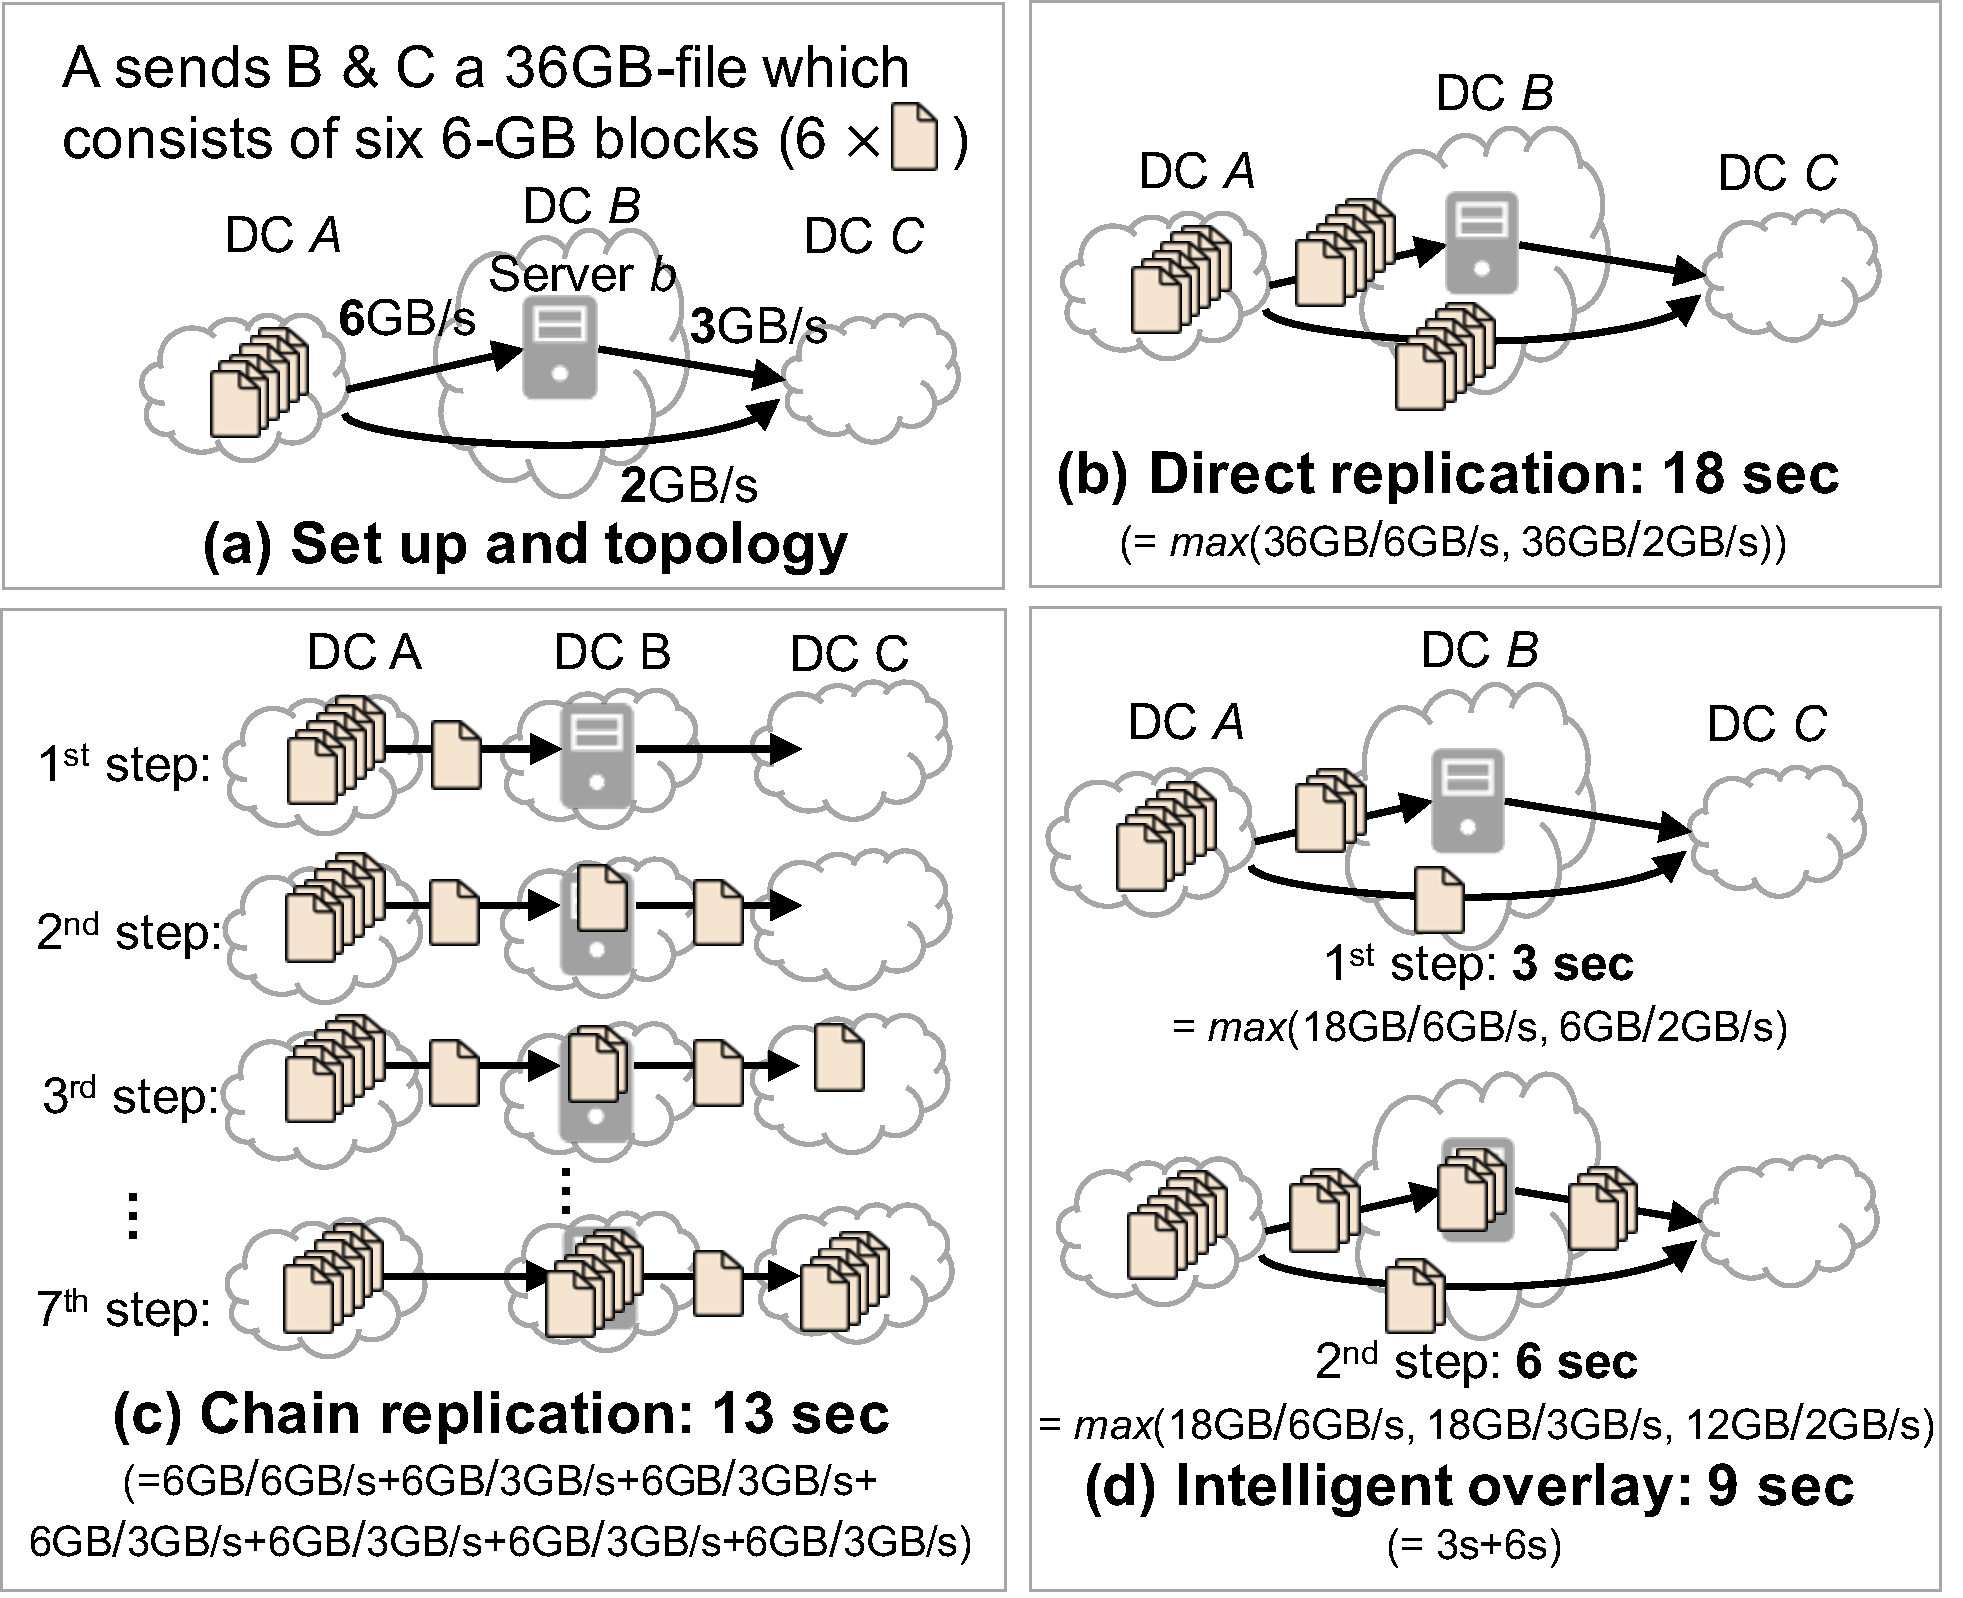
\includegraphics[width=84mm]{images/example-2.pdf}
\vspace{-0.4cm}
\tightcaption{An illustrative example comparing the performance of an intelligent application-level overlay (d) with that of baselines: naive application-level overlay (c) and no overlay (b).}
\label{fig:case:example}
\vspace{-0.4cm}
\end{figure}

It is known that, generally, multicast can be delivered using application-level
overlays~\cite{chu2000case}. Here, we show that inter-DC multicast
completion time (defined by the time until each destination DC has
a full copy of the data) can be greatly reduced by an
application-level overlay network. Note that an application-level
overlay does not require any network-level support, so it is
complementary to prior work on WAN optimization.

The basic idea of an application-level overlay network is to
distribute traffic along {\em bottleneck-disjoint} overlay
paths~\cite{datta19951}, i.e., the two paths do not share a common
bottleneck link or intermediate server.
In the context of inter-DC transfers, two overlay paths either
traverse different sequences of DCs ({\em Type I}), or
traverse different sequences of servers of the same sequence of
DCs ({\em Type II}), or some combination of the two.
%In Type I, the bottleneck can be in intermediate links or inside a DC,
%and in {\em Type II}, the bottleneck is likely to be inside a DC.
Next, we use examples to show bottleneck-disjoint overlay paths can
arise in both types of overlay paths and how they improve inter-DC
multicast performance.

\mypara{Examples of bottleneck-disjoint overlay paths}
In Figure~\ref{fig:intro}, we have already seen how two Type I overlay
paths ($A$$\rightarrow$$B$$\rightarrow$$C$ and
$A$$\rightarrow$$C$$\rightarrow$$B$) are bottleneck-disjoint,
and how it improves the performance of inter-DC multicast.
Figure~\ref{fig:case:example} shows an example
of Type II bottleneck-disjoint overlay paths
(traversing the same sequence of DCs but different sequence of
servers). Suppose we need to replicate 36GB data from DC $A$
to $B$ and $C$ via two bottleneck-disjoint paths:
(1) $A$$\rightarrow$$C$:
from $A$ through $B$ to $C$ using IP-layer WAN routing with
2GB/s capacity, or
(2) $A$$\rightarrow$$b$$\rightarrow$$C$: from $A$ to a server
$b$ in $B$ with
6GB/s capacity and $b$ to $C$ with 3GB/s capacity.
The data is split into six 6GB-blocks.
We consider three strategies.
(1) {\em Direct replication}:
if $A$ sends data directly to $B$ and $C$ via WAN paths
(Figure~\ref{fig:case:example}(b)),
the completion time is 18 seconds.
(2) {\em Simple chain replication}:
a naive use of application-level overlay paths
is to send blocks through server $b$ acting as a
store-and-relay point
(Figure~\ref{fig:case:example}(c)),
and the completion time is 13 seconds (27\% less than without overlay).
(3) {\em Intelligent multicast overlay}:
Figure~\ref{fig:case:example}(d) further improves the performance by
selectively sending blocks along the two paths simultaneously,
which completes in 9 seconds (30\% less than chain replication,
and 50\% less than direct replication).



\begin{figure}[t]
\centering
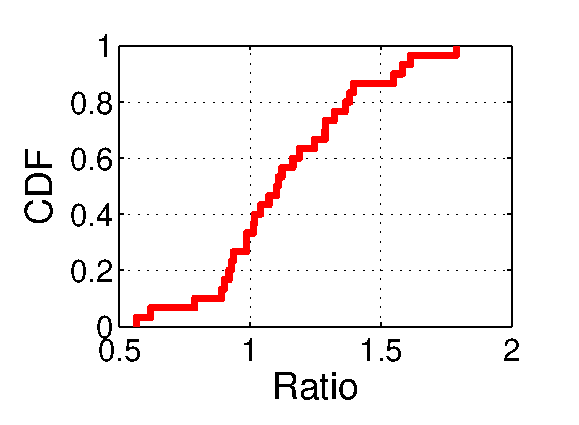
\includegraphics[width=1.5in]{images/potential_v2.eps}%DrawUp.m
\tightcaption{There is a significant performance variance among
the inter-DC overlay paths in our network, indicating that most
pairs of overlay paths are bottleneck disjoint.
%The figure shows the ratio between the available bandwidth
%from $A$ to $C$ through WAN ($BW_{A\rightarrow C}$) and
%that from $A$ to $C$ through $b$
%($BW_{A\rightarrow b\rightarrow C}$),
%across all possible $b$.
}
%\jc{drop (a). avoid using notions in figure captions. captions should be standalone}\jc{please use notations in consistent with those in the text}
\label{fig:case:size}
\vspace{-0.4cm}
\end{figure}

\mypara{Bottleneck-disjoint overlay paths in the wild}
It is hard to identify all bottleneck-disjoint overlay paths in our
network performance dataset, since it does not have per-hop bandwidth information of each
multicast transfer.
Instead, we observe that if two overlay paths have different end-to-end
throughput at the same time, they should be bottleneck-disjoint.
We show one example of bottleneck-disjoint overlay paths in the wild,
which consists of two overlay paths $A$$\rightarrow$$b$$\rightarrow$$C$
and $A$$\rightarrow$$C$, where the WAN routing from DC $A$ to DC $C$ goes
through DC $B$, and $b$ is a server in $B$ (these two paths are
topologically identical to Figure~\ref{fig:case:example}).
If $\frac{BW_{A\rightarrow C}}{BW_{A\rightarrow b\rightarrow C}}\neq1$,
they are bottleneck-disjoint ($BW_p$ denotes the throughput of path $p$).
Figure~\ref{fig:case:size} shows the distribution of
$\frac{BW_{A\rightarrow C}}{BW_{A\rightarrow b\rightarrow C}}$
among all possible values of $A$, $b$, and $C$ in the dataset.
We can see that more than 95\% pairs of $A$$\rightarrow$$b$$\rightarrow$$C$
and $A$$\rightarrow$$C$ have different end-to-end throughput, i.e.,
they are bottleneck disjoint.


\subsection{Limitations of existing solutions}
\label{subsec:motivation:baseline}

Realizing and demonstrating the potential improvement of an application-level
overlay network has some complications. As a first order approximation, we can
simply borrow existing techniques from multicast overlay networks
in other contexts. But the operational experience of \company shows
two limitations of this approach that will be described below.

\mypara{Existing solutions of \company}
To meet the need of rapid growth of inter-DC data replication,
\company has deployed \alg, an application-level overlay network a few
years ago. Despite years of refinement, \alg is based on a
receiver-driven decentralized overlay multicast protocol, which
resembles what was used in other overlay networks (such as CDNs and
overlay-based live video
streaming~\cite{Andreev2013Designing,sripanidkulchai2004analysis,zhang2005coolstreaming}).
The basic idea is that when multiple DCs request a data file from
a source DC, the requested data would flow back through multiple
stages of intermediate servers,  where the selection of senders in
each stage is driven by the receivers of the next stage in a
decentralized fashion.

\noindent{\bf Limitation 1:
Inefficient local adaptation.}
The existing decentralized protocol lacks the global view and thus
suffers from suboptimal scheduling and routing decisions.
To show this, we sent a 30GB file from one DC to two destination
DCs in \company's network. Each DC had 640 servers, each with 20Mbps
upload and download bandwidth (in the same magnitude of bandwidth
assigned to each bulk-data transfer in production traffic).
%\myfootnote{In \company, multiple services are mixed-deployed
%in the same DCs and even in the same servers, so server bandwidth is
%shared by many services and the available bandwidth for bulk data transfer is 20Mbps in general case}.
This 30GB file was evenly stored across all these 640 servers.
Ideally, if the servers select the best source for all blocks, the
completion time will be
$\frac{30\times 1024}{640\times 20Mbps \times 60s/min} = 41$
minutes. But as shown in Figure~\ref{fig:motivation},
servers in the destination DCs on average took 195 minutes (4.75$\times$
the optimal completion time) to receive data, and 5\% of servers even
waited for over 250 minutes.
The key reason for this problem is that individual servers only see a subset of
available data sources (i.e., servers who have already downloaded part of
a file), and thus cannot leverage all available overlay paths to
maximize the throughput. Such suboptimal performance could occur even if
the overlay network is only partially decentralized (e.g.,~\cite{Huang2014A}),
where even if each server does have a global view, local adaptations by
individual servers would still create potential hotspots and congestion on
overlay paths.


\begin{figure}[t]
  \centering
  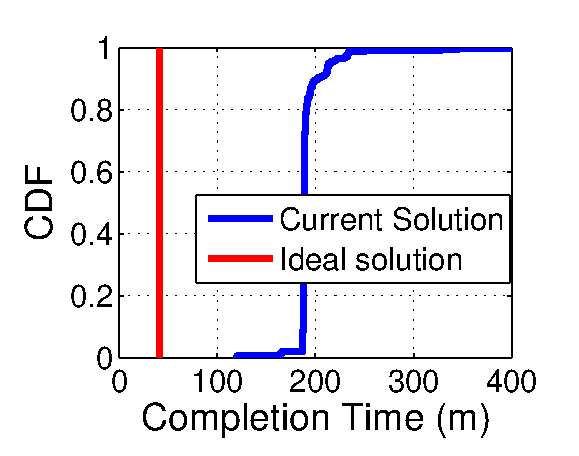
\includegraphics[width=1.5in]{images/SEvsIdeal.eps}
  \vspace{-0.2cm}
  \tightcaption{The CDF of the actual flow completion time at different servers in the destination DCs,
compared with that of the ideal solution. }
  \label{fig:motivation}
\vspace{-0.4cm}
\end{figure}

\noindent{\bf Limitation 2:
Interaction with latency-sensitive traffic.}
The existing multicast overlay network shares the same inter-DC WAN
with latency-sensitive traffic. Despite using standard QoS techniques,
and giving the lowest priority to bulk data transfers, we still see
negative impacts on latency-sensitive traffic by bursty arrivals of
bulk-data multicast requests. Figure~\ref{fig:lesson2} shows the
bandwidth utilization of an inter-DC link in two days during which a
6-hour long bulk data transfer started at 11:00pm on the second day.
The blue line denotes the outgoing bandwidth, and the green line
denotes the incoming bandwidth. We can see that the
bulk data transfer caused excessive link utilization (i.e., exceeding
the safety threshold of 80\%), and as a result, the latency-sensitive
online traffic experienced over 30$\times$ delay inflation.

\NEW{
\noindent{\bf Limitation 2: Low computation overhead.}

Decoupling of scheduling and routing.
}

\NEW{
\noindent{\bf Limitation 3: Real-time dynamic bandwidth separation.}

Prediction of online traffic.

Fine-granularity and near real-time schedule adjustment.
}


%The reason is that although all the servers worked under the standard QoS requirements, the excessive bandwidth usage of the inter-DC link still cannot be prevented due to lack of global coordination.


\begin{figure}[t!]
        \center
        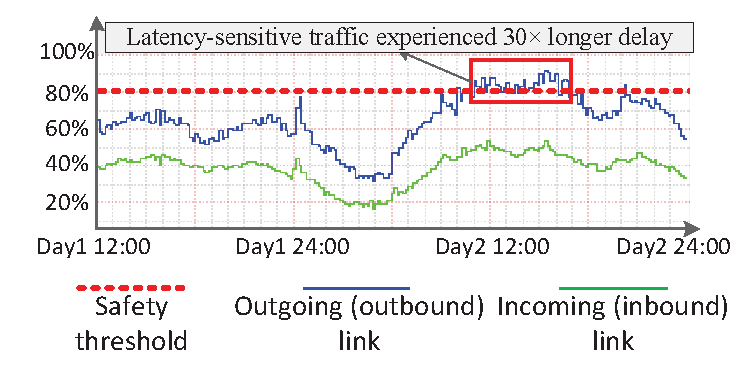
\includegraphics[width=3in]{images/nj02-M2A_0212-0216_v3.eps}
        \tightcaption{The utilization of the inter-DC link in two days. Inter-DC bulk data transfer on the 2nd day caused severe interference on latency-sensitive traffic.}
        \label{fig:lesson2}
\vspace{-0.4cm}
\end{figure}

\subsection{Key observations}
The key observations from this section are following:
\begin{packeditemize}
\item {\em Inter-DC multicasts} amount to a substantial fraction of
inter-DC traffic, have a great variability in source-destination, and
typically last for at least tens of seconds.
\item {\em Bottleneck-disjoint overlay paths} are widely available
between geo-distributed DCs.
\item Existing solutions that rely on local adaptation can have
{\em suboptimal performance} and {\em negative impact on
online traffic}.
\NEW{
\item {\em Real-time dynamic bandwidth separation} can be achieved if: online traffic can be predicted accurately and fine-granularity bandwidth adjustment can be conducted.
}
\end{packeditemize}

%\jc{can you say something like: such inefficiency is due to the inability
%to prevent exceeding bandwidth usage by bulk-data transfers in a
%decentralized manner}
%(1) Use a figure to show that bulk data transfer can cause significant delay on latency-sensitive traffic, and (2) put some concrete numbers to show such delay can cause significant revenue loss.

%\jc{can we show some numbers on how much delay on latency-sensitive traffic during that incident? and how much losses did it cause (either in terms of application quality or in \$\$)?}

%\end{itemize}


\section{Background}
\label{sec:motivation}

%\jc{Starting from Section 2, it would be paper outline.
%Please think each bullet point as a separate paragraph.}

%<<<<<<< HEAD
To motivate the need for an inter-DC multicast overlay,
we first characterize the workload of bulk-data multicast in
\company, a large-scale online service provider which has over
20 geographically distributed DCs
(\Section\ref{subsec:motivation:multicast-traffic}),
and then make a case for an intelligent inter-DC multicast
overlay network by showing that disjoint application-level
overlay paths are widely available and have great spatial
diversity in performance
(\Section\ref{subsec:motivation:case-for}).
Finally, we examine the existing multicast overlay networks
of \company, and draw important lessons from real-world incidents
and statistics (\Section\ref{subsec:motivation:baseline}),
which inform the design choices of \name.
%=======
%We begin by motivating the need for an inter-DC multicast overlay.
%We first characterize the bulk-data multicast workload in \company
%a large-scale online service provider
%(\Section\ref{subsec:motivation:multicast-traffic}),
%as there is relatively little study on DC-level multicast
%traffic.
%We then show
%a substantial diversity in performance of application-level
%overlay paths, and thus make a case for an inter-DC multicast
%overlay that picks optimal overlay paths to optimize bulk-data
%multicast.
%(\Section\ref{subsec:motivation:case-for}).
%Finally, we study the operational experience of \company, a large
%online service provider, and draw important lessons from
%real-world incidents and statistics
%of the \company's existing multicast protocol
%(\Section\ref{subsec:motivation:baseline}).
%>>>>>>> 09029e454f71e5a5e01f13f554477705e665f4ec


\subsection{Workload of bulk-data multicast}
\label{subsec:motivation:multicast-traffic}

\begin{table}[t]
\begin{center}
%\resizebox{\textwidth/2}{!}{
%\begin{tabular}{p{2cm}<{\centering}|p{2cm}<{\centering}}
\begin{tabular}{| c | c|}
\hline
 \rowcolor[gray]{0.9}
\textbf{Type of application} & \textbf{\% of multicast traffic} \\
\hline
All applications & 91.13\%~\footnotemark[2]\\
\hline
Blog posts & 91.0\% \\% 4648.92 vs 41372.56 in GB
\hline
Search indexing & 89.2\%\\% 16766.7 vs 138418.12
%\hline
%International & 98.15\%\\% 1297.7 vs 68699.97
\hline
Offline file sharing & 98.18\%\\% 2792.4 vs 150234.25
%\hline
%Scholar & 98.09\%\\% 451.22 vs 23134.21
\hline
Forum posts & 98.08\%\\% 964.62 vs 49327.01
\hline
Other DB sync-ups & 99.1\%\\% ?? vs ??
\hline
\end{tabular}
%}
\end{center}
\caption{DC-level multicast traffic (replicating data from
one DC to multiple DCs) dominantes the inter-DC traffic
in \company (across all applications and in
several important individual application types.}
\label{table:rate}
\end{table}
\footnotetext[2]{The overall multicast traffic
share is estimated by that of the traffic goes through one
randomly sampled DC, because we do not have access to
information of all inter-DC traffic, but this number is
consistent with what we observe on other DCs.}
%We randomly select one link from all inter-DC links whose traffic is monitored by different application types. As all these links carry the similar traffic, so the randomly selected one could exhibit good representatives.}


\mypara{Share of multicast traffic}
%<<<<<<< HEAD
First, we examine the share of inter-DC multicast traffic
(replicating data from one DC to multiple DCs)
as a fraction of all traffic.
Table~\ref{table:rate} shows multicast traffic as
a fraction of inter-DC traffic across all applications as
well as in some important application types individually.
We see that multicast traffic dominantes the inter-DC traffic
in \company, in terms of both overall traffic and
several important types of application traffic.
{\em The fact that inter-DC multicast traffic
amounts to a substantial share of inter-DC traffic
highlights the importance of optimizing multicast
traffic.}
%=======
%First, we use \company's WAN to examine whether
%inter-DC multicast traffic (replicating data from
%one DC to multiple DCs)
%amounts to a substantial share of inter-DC traffic.
%Table~\ref{table:rate} shows multicast traffic as
%a fraction of inter-DC traffic across all applications as
%well as in some important application types individually.
%We see that multicast traffic dominantes the inter-DC traffic
%in \company, in terms of both overall traffic and
%several important types of application traffic,
%which highlights the importance of optimizing multicast
%traffic.
%>>>>>>> 09029e454f71e5a5e01f13f554477705e665f4ec
%To check the percentage of multicast traffic, we breakdown all \company's total traffic volume into non-multicast traffic and the multicast traffic of each application, and then calculate the share of multicast traffic. Table \ref{table:rate} shows that a considerably large fraction of traffic is multicast traffic, despite the application types. This result highlights the importance of bulk-data transmission optimization.

\begin{figure}[t]
        \centering
        \begin{subfigure}[b]{0.23\textwidth}
                \centering
                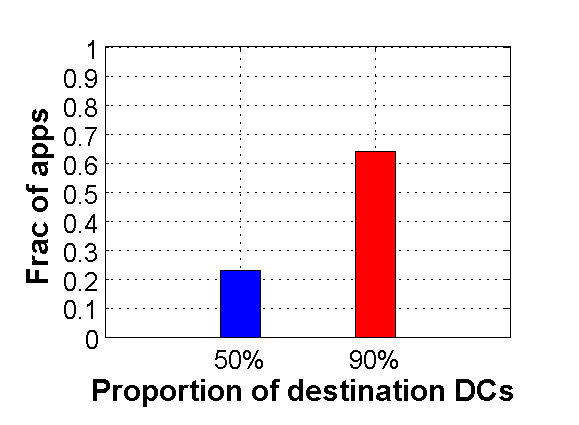
\includegraphics[width=\textwidth]{images/destinationDC.eps}%NeedMulticast.m
                \caption{\% of multicast transfers destined to \% of DCs.}
                \label{fig:bulk:dest}
        \end{subfigure}
	\hspace{0.1cm}
        \begin{subfigure}[b]{0.23\textwidth}
                \centering
                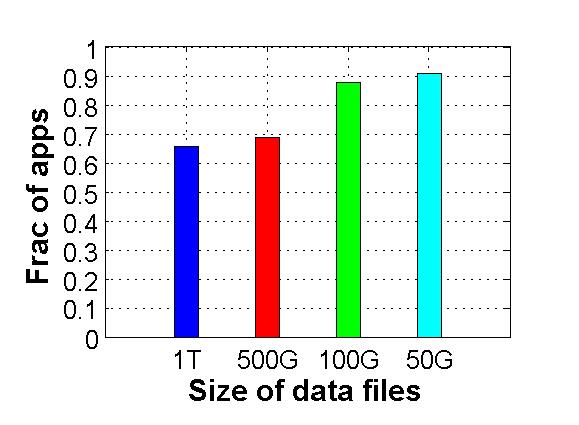
\includegraphics[width=\textwidth]{images/DataSize.eps}
                \caption{\% of multicast transfers larger than certain threshold.}
                \label{fig:bulk:size}
        \end{subfigure}
        \caption{Inter-DC multicast data transfers are (1) destined to a significant
fraction of DCs, and (2) huge in volume.}
        \label{fig:bulk}
\vspace{-0.4cm}
\end{figure}

\mypara{Destined to many DCs}
%<<<<<<< HEAD
Next, we examine whether these transfers are destined to the
a large fraction (or just a handful) of DCs.
Figure~\ref{fig:bulk:dest} sketches the distribution of the
percentage of DCs (in total, $\sim$ 30) to which multicast
transfers in \company are destined.
%=======
%In the premise that multicast traffic amount to a substantial
%fraction of traffic, we then examine whether these transfers
%are destined to just a handful of DCs.
%Figure~\ref{fig:bulk:dest} sketches the distribution of the
%percentage of DCs (in total, $\sim$ 30) to which multicast
%transfers are destined.
%>>>>>>> 09029e454f71e5a5e01f13f554477705e665f4ec
We can see that over 71\% of multicast transfers replicate data
to more than 80\% of DCs, and nearly 70\% of them are destined
to more than 60\% of DCs.
%<<<<<<< HEAD
Moreover, we also observed a great diversity  in terms of
source DCs and the sets of destination DCs (not shown here).
Together, these observations suggest that {\em it is not
scalable to pre-configure the multicast overlays as there
are many possible source-destination DCs.}
%=======
%Moreover, we observed a great diversity (not shown)
%in terms of source DCs and the sets of destination DCs.
%Together, these observations suggest that it is undesirable to
%pre-configure the multicast overlay.
%>>>>>>> 09029e454f71e5a5e01f13f554477705e665f4ec

%In the premise that bulk data shares a large fraction of overall traffic, we check the number of destination DCs of the data. Fig. \ref{fig:bulk:dest} shows that there are over 60\% applications with bulk data multicast traffic are destined to at least 90\% DCs, and about 20\% applications with bulk data destined to over 50\% (but less than 90\%) DCs. These results show that a large fraction of the bulk data traffic is multicast to almost all DCs.

\mypara{Carrying bulk data}
Finally, we examine the typical data size of multicast transfers.
Figure~\ref{fig:bulk:size} sketches the distribution of the
size of data files that need to be multicast in \company.
We see that over 60\% of multicast data files are larger than 1TB,
while 90\% of them are larger than 50GB.
%<<<<<<< HEAD
Such large data volumes suggest that the transfers are usually
long-lived, and thus {\em we should dynamically adjust
the routing scheme during a data transfer in response to
dynamic network performance.}
%=======
%The large data volumes suggest that the transfers are usually
%long-lived and thus we could improve multicast performance by
%routing data adaptively during a data transfer in response to
%dynamic network performance.
%>>>>>>> 09029e454f71e5a5e01f13f554477705e665f4ec


\vspace{0.1cm}
These findings indicate a strong need for a systematic approach
to optimizing inter-DC bulk-data multicast.

%To further explore the characteristics of the multicast data files, we summarize the data size of these files and present the statistical results in Fig. \ref{fig:bulk:size}, which shows that nearly 70\% applications have a data file larger than 1TB and over 90\% of these multicast applications have data files larger than 50GB. Thus, focusing on optimizing bulk data multicast transmission is quite valuable to improve WAN conditions.

%\begin{itemize}
%
%\item Share of multicast traffic: use a bar chart to show the breakdown of all Baidu's total traffic volume into non-multicast traffic, and the multicast traffic of each application. {\em This should show a large fraction of traffic is multicast, and they are from many different applications.}
%
%\item A CDF of number of destination DCs. {\em This should show that most multicast traffic are destined to almost all DCs.}
%
%\item A CDF of size of multicast data files. {\em This should show that most multicast data are bulk data (not small data), and thus focusing on optimizing bulk data multicast is valuable.}
%
%\end{itemize}

\subsection{A case for inter-DC multicast overlay}
\label{subsec:motivation:case-for}

%\begin{figure}[t]
%\centering
%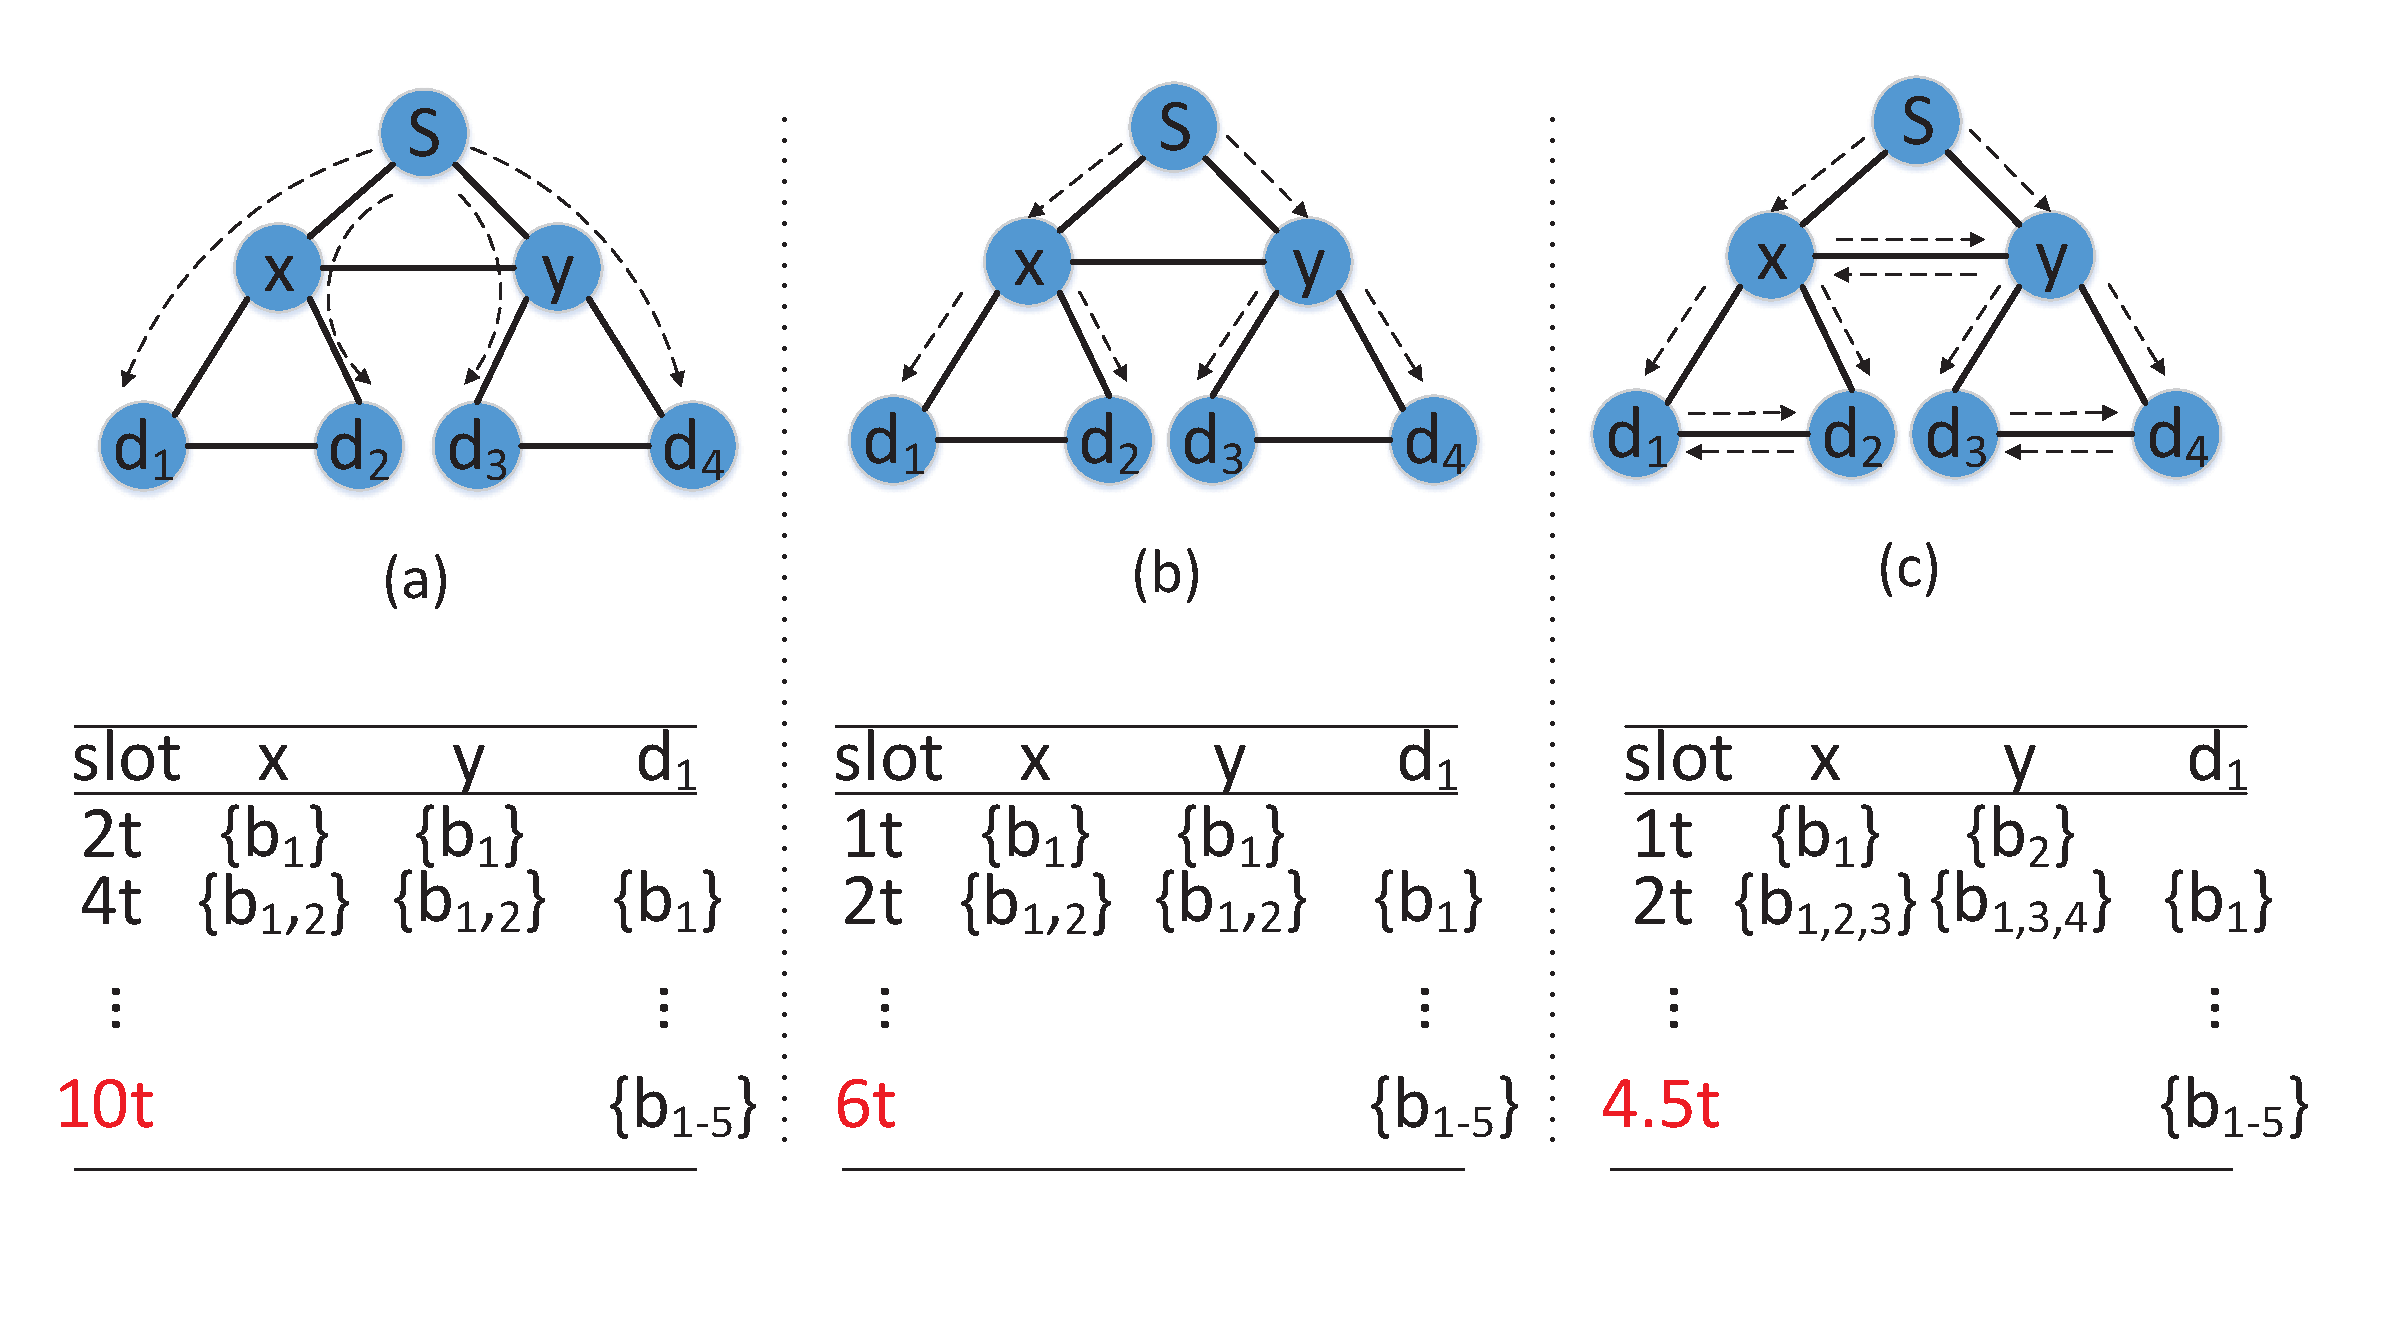
\includegraphics[width=80mm]{images/example.eps}
%\caption{A toy example showing the benefit from inter-DC multicast overlay.}
%\label{fig:case:example}
%\vspace{-0.4cm}
%\end{figure}

\begin{figure}[t]
\centering
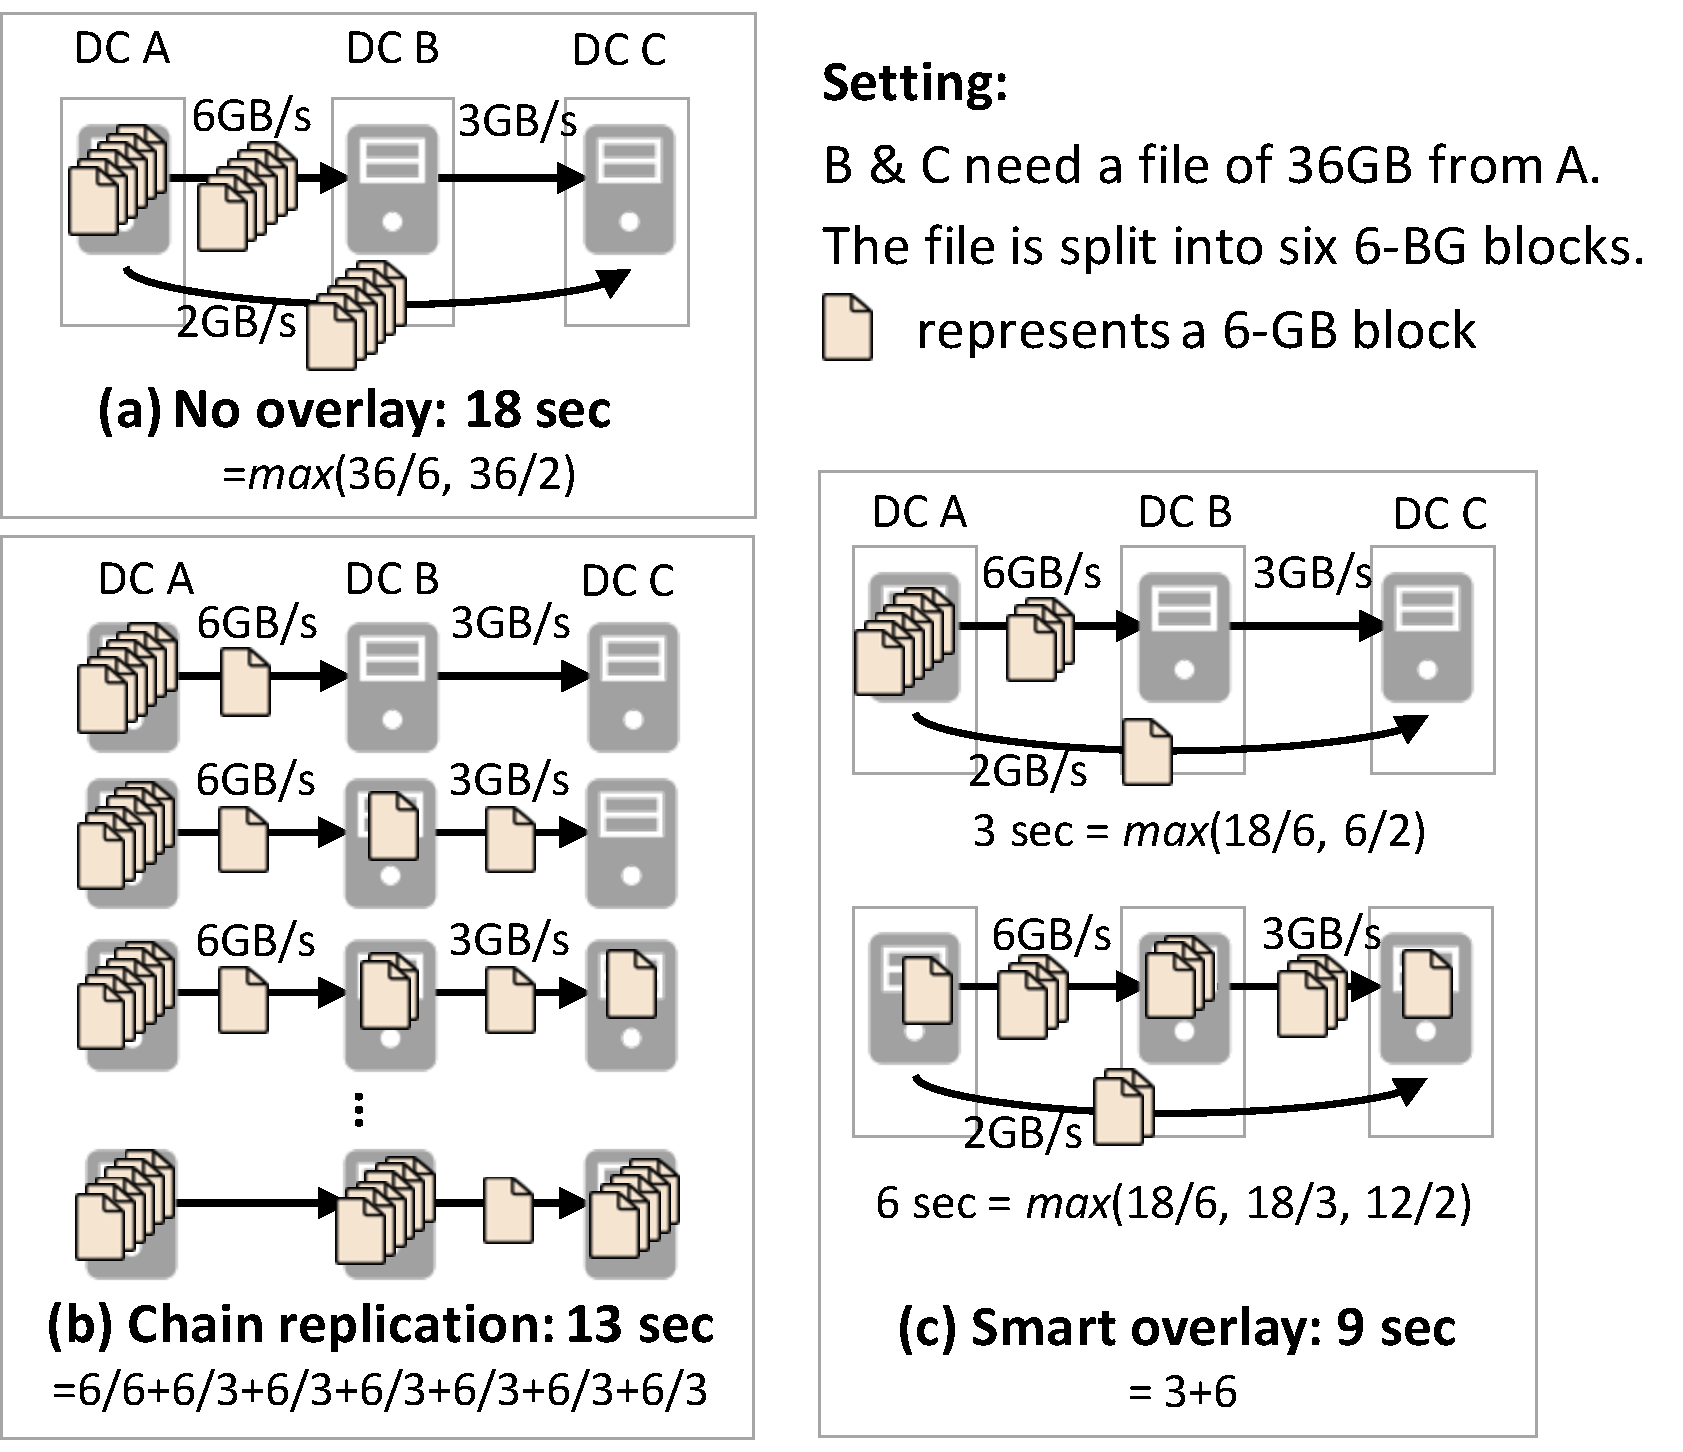
\includegraphics[width=80mm]{images/example-junchen.pdf}
\caption{A toy example showing the benefit from inter-DC multicast overlay.}
\label{fig:case:example}
\vspace{-0.4cm}
\end{figure}

The benefits of application-level overlays are well-known in
many contexts.
In this section, we first use an example  to
illustrate such benefits in the context of inter-DC bulk-data
multicast.

\mypara{An illustrative example}
As shown in Figure~\ref{fig:case:example},
suppose DC $B$ and $C$ want to fetch from DC $A$ a 36GB data file,
which has been chopped into six 6GB blocks.
(The transfer is completed as long as the data is fully received
by some servers in $B$ and $C$.)
%<<<<<<< HEAD
Topologically, $A$ is directly connected with $B$ by a 2GB/s
link, and $A$ has two paths to reach $C$: the WAN path
which has 2GB/s capacity
(note that this path could go through $B$), or an overlay path
from $A$ first to a server $b$ in $B$ with a 6BG/s link,
and then from $b$ to $C$ with a 3GB/s link.
To begin with, if $A$ sends the data directly to $B$ and $C$,
i.e., no application-level overlay,
as in Figure~\ref{fig:case:example}(a),
the completion time would be 18 seconds.
If we use overlay routing but with a simple DC-level chain
%=======
%Topologically, $A$ is directly connected to $B$, and
%$A$ has two paths to reach $C$: the WAN path
%which has 2GB/s capacity
%(note that this path could go through $B$), or the overlay path
%from $A$ to a server $X$ in $B$ with 6BG/s capacity,
%and then from $X$ to $C$ with 3GB/s capacity.
%To begin with, if $A$ sends the data directly to $B$ and $C$,
%as in Figure~\ref{fig:case:example}(a),
%i.e., no application-level overlay,
%the the completion time would be 18 seconds.
%If we use overlay routing but only with a simple DC-level chain
%>>>>>>> 09029e454f71e5a5e01f13f554477705e665f4ec
replication scheme, as shown in Figure~\ref{fig:case:example}(b),
it would take 13 seconds
to complete, already a 27\% decrease from 18 seconds.
However, we can further reduce the completion time
by judiciously scheduling blocks on different
overlay paths. For instance, Figure~\ref{fig:case:example}(c)
illustrates an overlay routing scheme which completes in 9
seconds, another 30\% decrease from 13 seconds.

The example of Figure~\ref{fig:case:example}
reveals a (well-known) observation that {\em the benefits of
application-level overlay networks depend critically on if
there exist disjoint paths between two nodes.}


%Fig. \ref{fig:case:example} shows three cases under different transmission strategies. Assume there are 6 DCs in the network: source DC \emph{S}, 2 intermediate DCs \emph{X} and \emph{Y}, 4 destination DCs $d_1,d_2,d_3,d_4$, and the bandwidth of both upload and download links are all 2Gbps. There is a 5G data file in the source DC \emph{S} that should be multicasted to all the 4 destination DCs. The data file is split into 5 blocks ($b_1,b_2,b_3,b_4,b_5$) each with 1G-size. (a) Directly sending data to each destination DC. The four source and destination pairs (s,d) share the link bandwidth fairly, and each is allocated to 0.5Gbps. Thus, the overall completion time in $d_i$ is 10t. (b) Build a multicast tree with chain replications on the intermediate DCs. Take $d_1$ as an example, his parent DC \emph{X} could begins to send $b_1$ with 1Gbps at the beginning of 2nd time slot because \emph{X} has already duplicated $b_1$ after 1t. So that the completion time can be reduced to 6t. (c) An optimal solution on multicast overlay network. \emph{S} sends different blocks to \emph{X} and \emph{Y} in the 1st time slot to make them share those block mutually in the next slot. Thus, in the end of 2nd slot, both \emph{X} and \emph{Y} have 3 blocks. Similarly, $d_1$ and $d_2$ are also able to share complementary blocks while download the other blocks from parent DC simultaneously. The completion time can then be further reduced to 4.5t.

\begin{figure}[t]
\centering
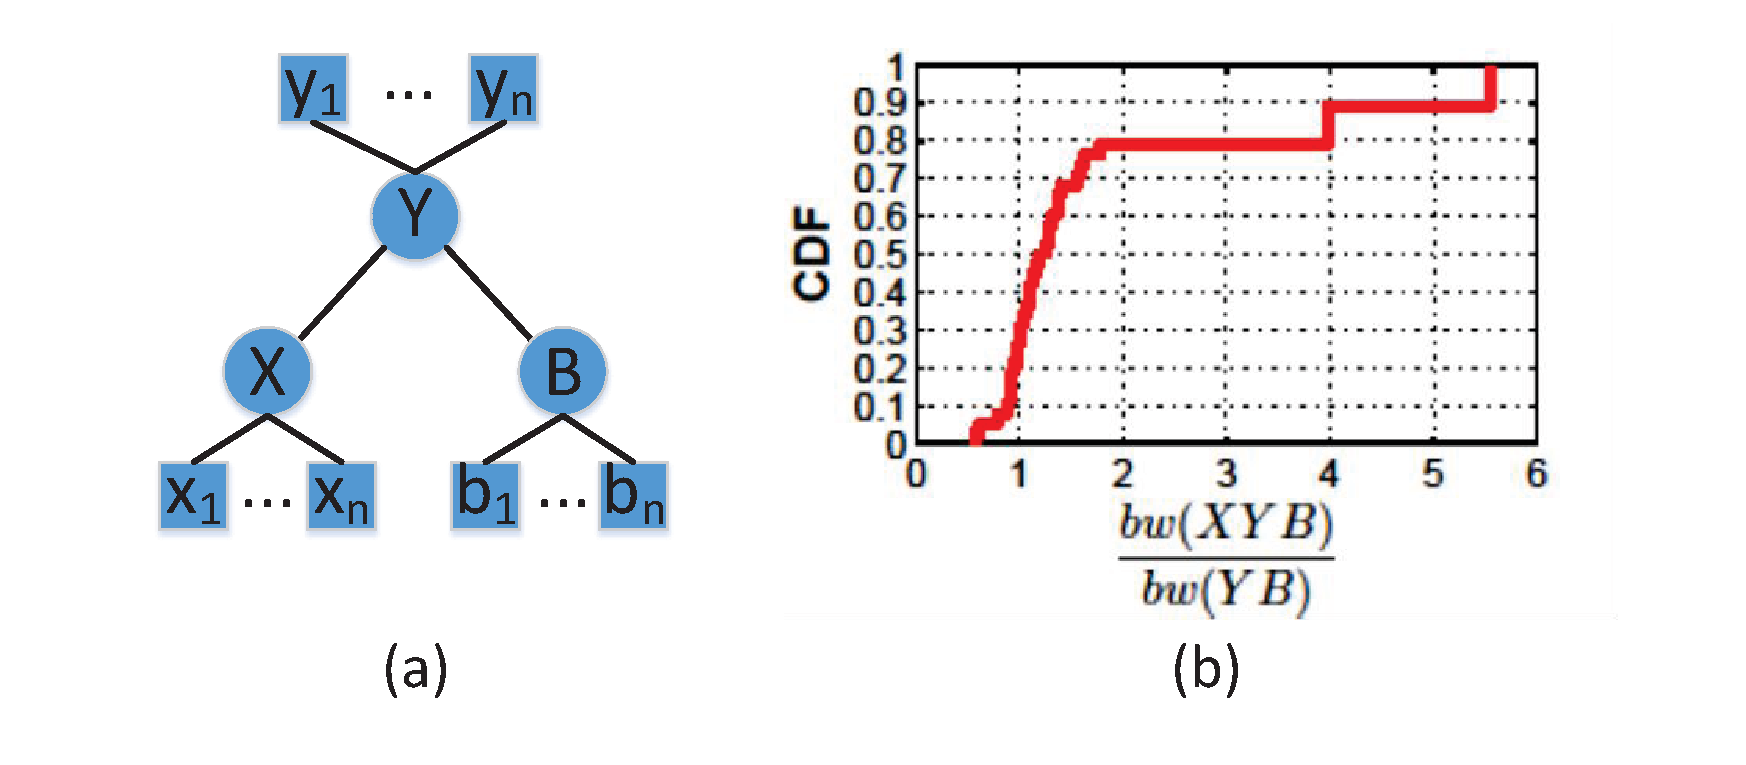
\includegraphics[width=80mm]{images/potential.eps}%DrawUp.m
\caption{Measurements showing the potential bandwidth between different (s,d) pairs.}
\label{fig:case:size}
\vspace{-0.4cm}
\end{figure}

%<<<<<<< HEAD
\mypara{Potential benefits in the wild}
We argue that the benefits illustrated in the example of
Figure~\ref{fig:case:example} can be actually realized in a
real DC WAN. The intuition is that
global-scale online service providers,
such as Google and \company, have disjoint paths in abundance,
both at DC-level (e.g., consider B4~\cite{b4}'s WAN topology)
and at server-level (e.g., consider Figure~\ref{fig:case:example}
where depending on the intermediate server $b$ in $B$,
$A$ has many overlay paths to $C$).
A crucial question, however, is that while two overlay paths are
physically disjoint, they might share the same bottleneck, and
thus should be counted as not disjoint in our context.
Here, we answer the question under a case for which physically
disjoint paths share network bottlenecks.
When two overlay paths go through different servers but traverse
the inter-DC WAN path, they would tend to have the same network
bottlenecks, as WAN capacity is usually believed to be more
limited than intra-DC networks.
However, our empirical measurement in \company's networks shows
otherwise.
We consider three DCs from \company's WAN that have the same
connectivity as in Figure~\ref{fig:case:example},
and show the distribution of
$\frac{BW_{A\rightarrow C}}{BW_{A\rightarrow b\rightarrow C}}$,
the ratio between the available bandwidth
from $A$ to $C$ through WAN ($BW_{A\rightarrow C}$) and
that from $A$ to $C$ through $b$
($BW_{A\rightarrow b\rightarrow C}$),
across all possible choices of $b$.
If WAN is indeed the bandwidth bottleneck, we should see
$\frac{BW_{A\rightarrow C}}{BW_{A\rightarrow b\rightarrow C}}=1$,
but the graph shows a substantial discrepancy between
$BW_{A\rightarrow C}$ and $BW_{A\rightarrow b\rightarrow C}$,
indicating that the available bandwidth can be bottlenecked by
the capacity of server $b$
($BW_{A\rightarrow C}>BW_{A\rightarrow b\rightarrow C}$),
or the intra-DC network in DC $B$
($BW_{A\rightarrow C}<BW_{A\rightarrow b\rightarrow C}$).
These observations corroborate the intuition that
{\em many physically
disjoint overlay paths tend not to share bottleneck}.

%=======
%\mypara{Opportunities in the wild}
%Next, we use performance measured from \company's DC servers to
%investigate whether the benefits illustrated by
%Figure~\ref{fig:case:example} can be realized in a real DC WAN.
%The example of Figure~\ref{fig:case:example}
%reveals a well-known observation that the benefits of
%application-level overlay networks depend critically on if
%there exist disjoint paths between two nodes that have diverse
%performance.
%We argue that global-scale online service providers such as Google
%and \company have such disjoint paths in abundance.
%First, the disjoint paths can emerge both
%at DC-level (e.g., consider B4~\cite{b4}'s WAN topology) and
%at server-level (e.g., consider Figure~\ref{fig:case:example}
%where depending on the intermediate server in $B$,
%$A$ has many overlay paths to $C$, all via the same DC-level
%path).
%Next, we use Figure~\ref{fig:case:size} show that these paths
%have substantially diverse performance.
%We consider three DCs from \company's WAN that have the same
%connectivity as in Figure~\ref{fig:case:example}.
%We randomly selected
%>>>>>>> 09029e454f71e5a5e01f13f554477705e665f4ec


%Consider the abstract topology of \company's real network, we can also find the situations similar to the above example. There are several DC groups divided by geographical locations, and every two groups are connected through one fiber link with high bandwidth. Within each DC group, there are dozens of DCs, and in each DC, there are normally 10,000 servers. Thus, there are numbers of possible disjoint paths between any DC pairs.

%To intuitively show the benefit from disjoint paths, we make the follow measurements on the available bandwidth among three DC groups \emph{X, Y, B}. The topology is shown in Fig. \ref{fig:case:size}(a). $x_i,y_i$ and $b_i$ are servers in \emph{X, Y, B}, while any server in \emph{X} needs to go through \emph{Y} to get to any arbitrary server $b$ in \emph{B}. Let $bw(XYB)$, $bw(YB)$ denote the bandwidth between $x_i$ and $b_k$, and between $y_j$ and $b_k$, respectively, we show the fraction of $bw(XYB)$ and $bw(YB)$ in Fig. \ref{fig:case:size}(b). This figure illustrates that only in a few case (about 20\%), the available bandwidth between \emph{Y} and \emph{B} is higher than that between \emph{X} and \emph{B}, while in the majority of cases, $\frac{bw(XYB)}{bw(YB)}>1$, meaning selecting senders is not straightforward, and we do need to consider large decision spaces.

%\begin{itemize}
%
%\item Give an illustrative toy example to compare (1) directly sending data to each destination DC, (2) use chain replication, i.e., build a multicast tree with each DC being a node, (3) an optimal solution.
%{\em\bf This example is critical!}
%
%\item Briefly explain the basics of Baidu's inter-DC WAN: topology, \# of servers per DC, some estimates on how many disjoint paths are available between two DCs.
%{\em The point is that each DC has multiple disjoint paths to fetch data, despite a seemingly tree-like topology.}
%
%\item Show a CDF of $\frac{X_i\rightarrow B}{Y_i\rightarrow B}$, where $X_i\rightarrow B$, $Y_j\rightarrow B$ are the bandwidth between some server in $X$ and $B$, and between some server in $Y$ and $B$, respectively. Assume $X$ needs to go through $Y$ to get to $B$.
%{\em The point is that in a substantial fraction of cases, $\frac{X_i\rightarrow B}{Y_i\rightarrow B}>1$, meaning selecting the sender is not straightforward, we do need to consider large decision space.}
%
%\end{itemize}

\subsection{Limitations of existing solutions}
\label{subsec:motivation:baseline}

\begin{figure*}[t]
        \center
        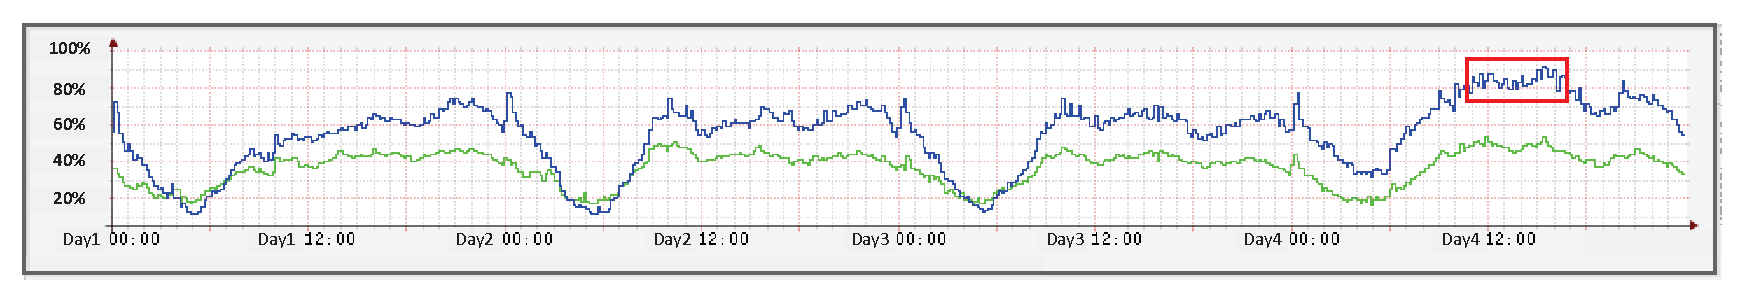
\includegraphics[height=25mm,width=150mm]{images/nj02-M2A_0212-0216.eps}
        \caption{Bulk data transfer on the 4th day caused significant traffic burst.
        \jc{remove the first few days, only show the last day, and make it single column}}
        \label{fig:lesson2}
%\vspace{0.1in}
\end{figure*}

We have seen that inter-DC multicast overlay networks have
promising potentials in optimizing inter-DC bulk-data multicast.
Realizing such potential in practice, however, 
is easier said than done.
At a first glance, it seems we can borrow existing techniques 
from other multicast overlay systems, which logically solves a 
similar problem.
However, drawing on \company's experience deploying and evolving
its multicast overlay networks, we identify two limitations of
applying existing multicast overlay protocols in inter-DC bulk 
data multicast.

\mypara{Existing solution}
A few years ago, to meet the need of rapid growth in multicast
data, \company deployed a simple
receiver-driven decentralized protocol, which 
was similar to what was used in other overlay networks
(such as CDNs and overlay video streaming)
where multicast is needed. 
Since then \company has been improving the multicast overlay 
network for over five years, but the basic workflow of 
data requests remains the same.
At a high level, when multiple DC wants to download a data
file, they send the request to the source DC, and then the
requested data would flow back through multiple stages of 
intermediate servers, where the selection of senders in each stage 
is driven by the receivers of the next stage in a decentralized
fashion.
This basic workflow resembles many state-of-the-arts overlay 
protocols designed and deployed to realize large-scale live video 
streaming~\cite{??,??}.
%For the intermediate DCs, there is a customized store-and-forward strategy that decides whether to store the data or not and when to delete the data.
%The being used protocol in \company is a receiver-driven decentralized protocol. Once a receiver wants to download a data file, it announces the requirement to the source DC, then the required data will be forwarded to it through both the source DC and intermediate DCs. For the intermediate DCs, there is a customized store-and-forward strategy that decides whether to store the data or not and when to delete the data.
%This solution has been running for more than five years and has been continuously improved over time.

%At the same time, there are also some other solutions. For example, layered structures of DCs \cite{??} could simplify the scheduling and routing algorithm in the latency-sensitive systems but cannot explore more potential spaces and thus far from being optimal. Some pair-wise solutions like \cite{b4,bwe} improving inter-DC scheduling and routing are also not sufficient in the multicast overlay networks, due to the ignorance of multiple overlay paths.

%\mypara{Key limitations}
%To sum up, we can get two key lessons from the current baseline solutions.
As the inter-DC traffic continues to explode and more DCs are 
deployed, this protocol has begun to show two limitations.

\begin{figure}[t]
        \centering
        \begin{subfigure}[b]{0.23\textwidth}
                \centering
                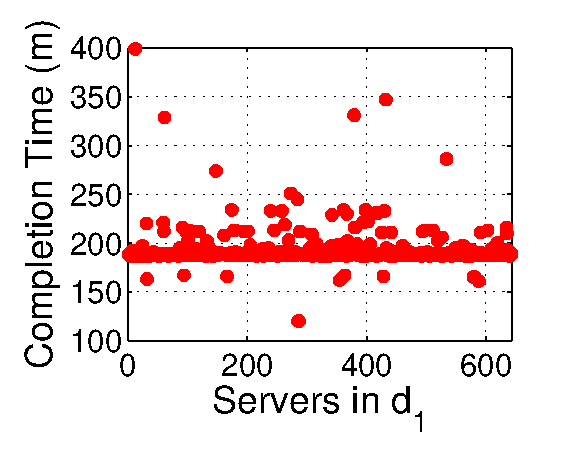
\includegraphics[width=\textwidth]{images/SE_3.eps}
                \caption{The completion time of the 643 servers.}
                \label{fig:motivation:observation1}
        \end{subfigure}
        \begin{subfigure}[b]{0.23\textwidth}
                \centering
                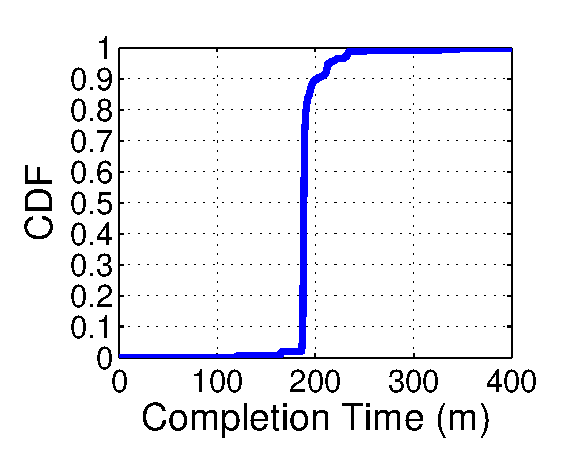
\includegraphics[width=\textwidth]{images/SE_3_cdf.eps}
                \caption{The CDF of transmission completion time.}
                \label{fig:motivation:observation2}
        \end{subfigure}
        \caption{The completion time under the current baseline solution. \jc{drop (b). add a line of 41minutes to (a). }}
        \label{fig:motivation}
\vspace{-0.4cm}
\end{figure}

%\begin{itemize}
%\item Briefly describe how \company does multicast today: how to data is forwarded through an intermediate DC? what's the protocol (a receiver-driven decentralized protocol)?
%We should also stress that this solution has been running for \fillme years and has been continuously improved over time.
%
%\item Briefly mention other solutions (layered structure, hybrid approach, and why not optimizing pair-wise DC link is not sufficient)


\noindent{\bf Limitation 1: 
Inefficiency due to the price of anarchy.}
The existing decentralized protocol lacks the global information 
about the whole network, and thus cannot make optimal scheduling. 
To show this, we run an experiment under a simplest topology that 
there is 1 source DC $s$ and 2 destination DCs $d_1, d_2$ 
(there are 640 servers in each DC), transferring a 30GB data file 
on $s$ to $d_1$ and $d_2$, with 20Mbps upload and download 
bandwidth. 
Theoretically, the optimal overlay solution could always select 
the better source for any block of the data file, and the ideal 
completion time for $d_1$ and $d_2$ is 
$\frac{30\times 1024}{640\times 20Mbps \times 60s/min} = 41$ 
minutes. 
Figure~\ref{fig:motivation} shows the results under the existing 
protocol. We see that the average completion time is about 
195 minutes, 4.75$\times$ longer than the optimal completion time. 
What's worse, it also exhibits heavy tail latency and there are 
about 5\% servers whose completion time is more than $200min$.

%\jc{this is still a toy example. we want to use real data to show these observations. how about using the previous figure to show tail latency.}

\noindent{\bf Limitation 2: 
Interference with latency-sensitive traffic.}
The existing multicast overlay network share the same inter-DC WAN 
with latency-sensitive traffic. 
Despite using standard QoS technique and giving the lowest priority to 
bulk data transfers, we still see frequent interference with 
latency-sensitive traffic caused by bursty arrival of bulk data 
requests.
We continuously monitored the bandwidth utilization of an inter-DC 
link in four days where there is a bulk data transfer at 11:00 on the 
4th day (lasted for 6 hours and finished at 17:00). 
Figure~\ref{fig:lesson2} shows the link utilization during the four 
days, from which we can see that the bulk data transfer caused 
significant traffic burst. As a result, the latency-sensitive online 
traffic that runs simultaneously on this link therefore suffered over
30 times longer delay, usually speaking, 
from about $60ms$ to nearly 2 seconds.
%(1) Use a figure to show that bulk data transfer can cause significant delay on latency-sensitive traffic, and (2) put some concrete numbers to show such delay can cause significant revenue loss.

%\jc{can we show some numbers on how much delay on latency-sensitive traffic during that incident? and how much losses did it cause (either in terms of application quality or in \$\$)?}

%\end{itemize}



%\NEW{
\section{System Overview}
\label{sec:overview}
To optimize inter-DC multicasts, while dynamically separated with
latency-sensitive traffic, we present {\em \name}, a {\em fully centralized} near-optimal network system with dynamic bandwidth separation for data inter-DC multicast.} Before presenting the details, we first highlight the intuitions behind the design choices, the challenges to make it practical.


\mypara{Centralized control}
Conventional wisdom on wide-area overlay networks has relied, to
some extent, on {\em local} adaptation of individual nodes (or
relay servers) to achieve desirable scalability and responsiveness
to network dynamics
(e.g.,~\cite{Andreev2013Designing,Repantis2010Scaling,Huang2014A,mukerjee2014enabling}),
despite the resulting suboptimal performance due to lack of global
view or orchestration.
%Recent work (e.g.,~\cite{mukerjee2014enabling}), however,
%shows the feasibility of combining
%local adaptation with a centralized logic operating
%on coarse timescales.
In contrast, \name takes an explicit stance that it is practical to
fully centralize the control of wide-area overlay networks and
still achieve near-optimal performance in the setting of inter-DC
multicasts. This design coincides other recents works of centralizing
management of large-scale distributed systems, e.g.,~\cite{gog2016firmament}
At a high level, \name uses a centralized controller that
periodically pulls information (e.g., data delivery status) from all
servers, updates the decisions regarding overlay routing, and pushes
them to agents running locally on servers
(Figure~\ref{fig:framework}).
Note that when the controller fails or is unreachable, the system will
fall back to a decentralized control scheme to ensure graceful
performance degradation to local adaptation
(\Section\ref{subsec:system:fault}).

\begin{figure}[t]
  \centering
  %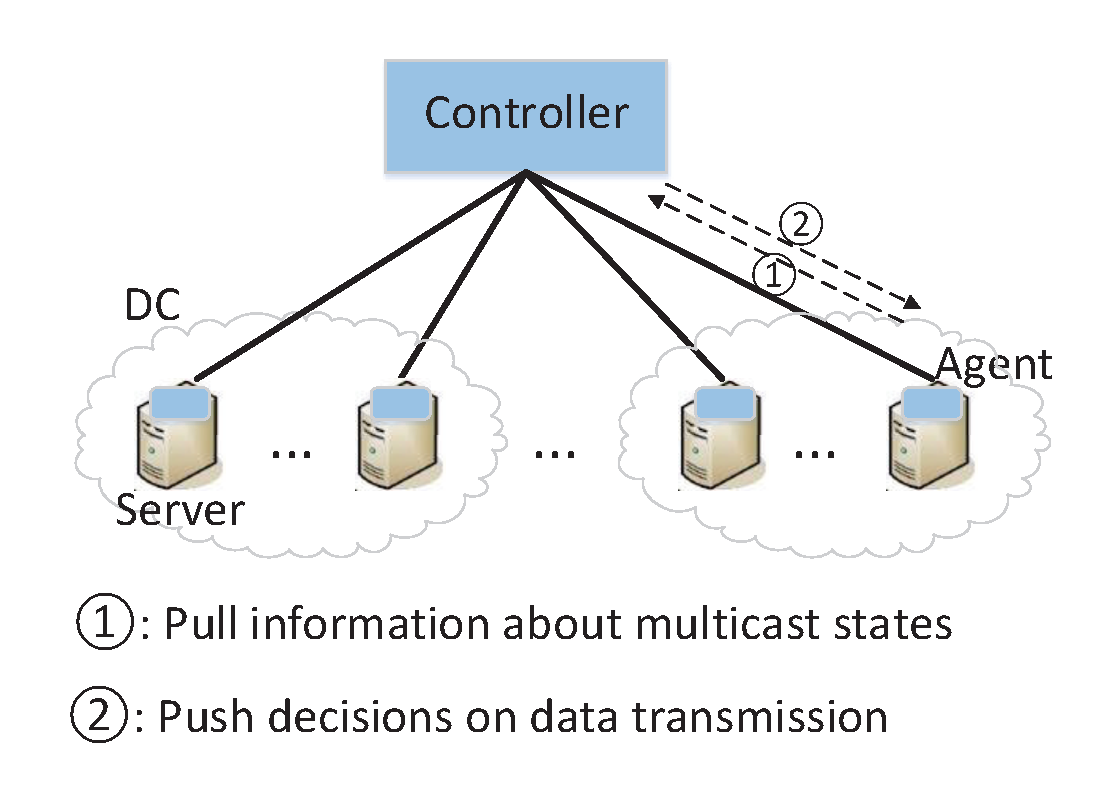
\includegraphics[width=2in]{images/framework.eps}
  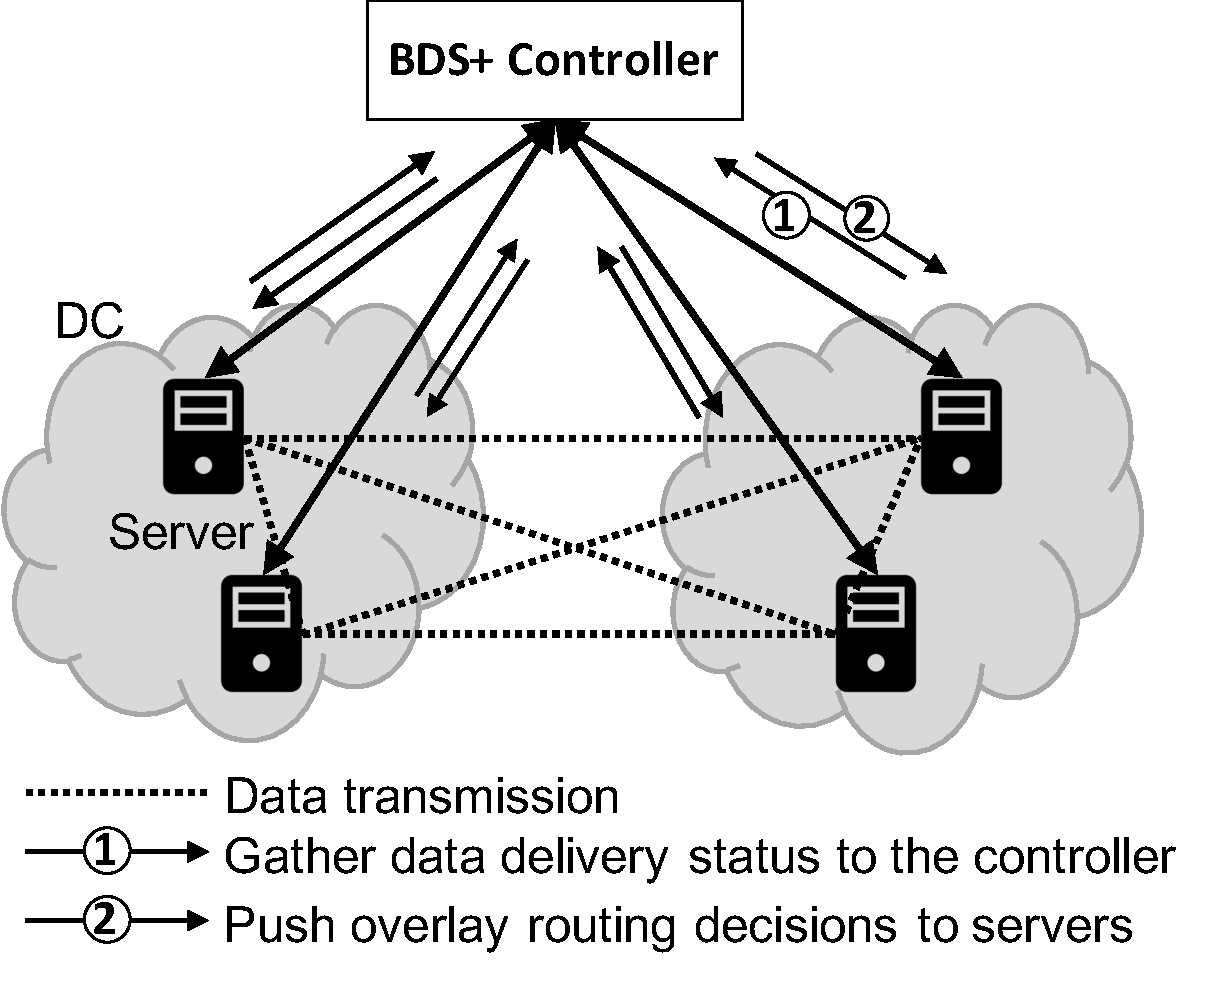
\includegraphics[width=2.3in]{images/framework-journal.pdf}
    \vspace{-0.2cm}
  \tightcaption{The centralized design of \name.}
  \label{fig:framework}
\vspace{-0.4cm}
\end{figure}

Our centralized design is driven by several empirical observations:
\begin{packedenumerate}

\item {\em Large decision space:}
The sheer number of inter-DC overlay paths (which grow exponentially
with more servers acting as overlay nodes) makes it difficult for
individual servers to explore all available overlay paths based only
on local measurements. In contrast, we could significantly improve
overlay multicast performance by maintaining a global view of data
delivery status of all servers, and dynamically balancing the
availability of various data blocks, which turns out to be critical
to achieving near-optimal performance
(\Section\ref{subsec:logic:scheduling}).

\item {\em Large data size:}
Unlike latency-sensitive traffic which lasts
on timescales of several to 10s of milliseconds, inter-DC multicasts
last on much coarser timescales.
%Thus, it is a necessary requirement to be continously adaptive to
%any transient network dynamics.
%In this context, the tradeoff between a centralized design and a decentralized one is that centralized control essentially trades real-time responsiveness to network dynamics for closer-to-optimal control decisions driven by a global view of data delivery. Here,
Therefore, \name can tolerate a short delay (of a few seconds) in order
to get better routing decisions from a centralized controller which
maintains a global view of data delivery and is capable of orchestrating
all overlay servers.

\NEW{
\item {\em Flexible traffic control:}
Previous works~\cite{Andreev2013Designing,Repantis2010Scaling,Huang2014A,mukerjee2014enabling} use the static separation scheme where there is a fixed boundary between online and offline traffic, here \name proposes to use dynamic bandwidth separation, so it should know the bandwidth utilization in a global view, in order to dynamically adjust the amount of available bandwidth that can be used for bulk-data transfer. Once any network changes are detected, \name could easily adjust bandwidth for each data transfer by controlling the sending rate at all servers in a centralized fashion (nomatter to reserve more bandwidth when online traffic burst, or to reduce transfer rate when online traffic is in valley).
(\Section\ref{sec:deployment}).
}

\item {\em Lower engineering complexity:}
Conceptually, the centralized architecture moves the control
complexity to the centralized controller, making \name amenable to a
simpler implementation, in which the control logic running locally in
each server can be stateless and triggered only on arrivals of new
data units or control messages.

\end{packedenumerate}

%\mypara{Fast and near-optimal decision-making}
\mypara{The key to realizing centralized control}
In essence, the design of \name performs a trade-off between incurring
a small update delay in return for the near-optimal
decisions brought by a centralized system. Thus, the key to striking such a
favorable balance is a near-optimal yet efficient overlay routing
algorithm that can update decisions in near realtime. At a first
glance, this is indeed intractable. For the workload at a scale of
\company, the centralized overlay routing algorithm must pick the next
hops for $10^5$ of data blocks from $10^4$ servers. This operates at a scale that
could grow exponentially when we consider the growth in the number of possible
overlay paths that go through these servers and with finer grained
block partitioning. With the standard routing formulation and linear
programming solvers, it could be completely unrealistic to make
near-optimal solutions by exploring such a large decision space
(\Section\ref{subsubsec:evaluation:depth}).

\NEW{
\mypara{The key to realizing dynamic bandwidth separation}
Dynamic bandwidth separation raises two requirements, one is to reserve enough bandwidth for latency-sensitive online traffic so as to avoid negative impacts on these services, and the other is to make full use of the residual bandwidth so as to reduce the completion time of bulk data transfer. With the traditional strict safety threshold and decentralized protocols, it could be impossible to make efficient bandwidth usage in the dynamic and mixed deployed network (\Section\ref{subsec:evaluation:improvements}).
}

The following two section will present how \name works.


%\section{Design Overview of \name}
\label{sec:overview}

To optimize inter-DC bulk-data multicast while avoiding
interference with latency-sensitive traffic, we present \name,
a near-optimal inter-DC multicast overlay network.
\name is built on a couple of design choices, which
%To optimize the performance of bulk-data replication, \name
%addresses the key challenges of a multicast overlay network
%by two design choices, both of which
trade marginal costs for substantial performance benefits.
Before describing the details of \name's design, we first
highlight the design choices and the intuition behind
their cost-benefit tradeoffs
(summarized in Table~\ref{tab:design-choices}).

\jc{add a figure here to illustrate the centralized
architecture?}

%The insights obtained from \company's operational experience has inspired the design of \name, a near-optimal inter-DC multicast overlay network. This section starts with \name key design choices, highlights the design philosophy behind our choices, and provide an overview of the \name system, which builds on these design choices.

\subsection{Design choices}

\mypara{Centralized decision-making}
\name uses a centralized controller to periodically poll
the data delivery status from all servers, and
updates the overlay path selection and bandwidth allocation
accordingly.
The benefits of the centralized decision-making are
two-fold.
First, having a global view on which data each server has
received enables exploring a large set of possible
overlay servers to circumvent performance bottlenecks,
which would be otherwise impossible.
Second, the centralized view allows us to
balance the number of intermediate overlay nodes of different
data blocks, which is shown in \Section\ref{subsec:logic:scheduling}
to be critical to
achieving optimal overlay multicast performance.

%Our first design choice is the fully centralized control. For large online service providers like \company, there are considerably large number of servers and exponentially more overlay paths, so it is hard to find out the optimal one for any decentralized solutions with only local information. \name, however is able to make near-optimal overlay routing and scheduling decisions with a centralized decision-making scheme. Furthermore, the embedded controller is lightweight in terms of CPU, bandwidth consumed, and thus enjoys good scalability over WANs.


\mypara{Clean bandwidth separation}
To prevent delay caused on the latency-sensitive user data,
\name separates background bulk data transfers from
latency-sensitive traffic.
The \name controller continuously monitors the aggregated
volume of each traffic category (e.g., bulk data transfers,
latency sensitive short flows), dynamically
determines how much residual bandwidth should be allocated to
multicasting bulk data, and enforces a clean separation of
bandwidth between bulk data transfers and latency-sensitive
traffic.

%The second design choice is dynamic bandwidth separation. To prevent delay caused on the latency-sensitive user data, \name separates background bulk data transfer from latency-sensitive traffic. Specifically, \name maintains the information of all links and monitors the aggregated traffic from all latency-sensitive data, thus can dynamically calculate the residual bandwidth that can be allocated for background bulk data transfer. This clean bandwidth separation can efficiently prevent interference on latency-sensitive traffic.


\begin{table}[t]
\centering
\begin{small}
\begin{tabular}{lll}
\textbf{Design choices} & \textbf{Benefits} & \textbf{Costs} \\ \hline
\textit{\begin{tabular}[c]{@{}l@{}}Centralized \\ decision-making\end{tabular}} & \begin{tabular}[c]{@{}l@{}}Optimal control based \\ on a global view\end{tabular} & \begin{tabular}[c]{@{}l@{}}Unable to update \\ decision in realtime\end{tabular} \\ \hline
\textit{\begin{tabular}[c]{@{}l@{}}Clean bandwidth \\ separation\end{tabular}} & \begin{tabular}[c]{@{}l@{}}Less interference with\\ latency-sensitive data\end{tabular} & \begin{tabular}[c]{@{}l@{}}Relatively lower \\ link utilization\end{tabular}
\end{tabular}
\end{small}
\caption{\name's design choices and their benefit-cost tradeoffs}
\label{tab:design-choices}
\end{table}

\subsection{Design philosophy}

These benefits of \name's design choices do not come for free.
On one hand, \name's centralized architecture creates an unwieldy
decision-making process that is difficult to update in real time
(due to the prohibitively large scale of the problem),
or with the most up-to-date global view (due to inherent latency
to gather data from globally distributed servers).
On the other hand, enforcing a fixed split on bandwidth resource
could result in low link utilization, if such split is adjusted on
a coarser timescale than the speed of traffic demand fluctuation.

%The above two design choices may introduce performance costs, i.e., fully centralized control makes \name unable to update decisions in real time, because the \name controller works in a centralized manner and has to collect information from geo-distributed DCs, and this will naturally introduce some communication latency to the decision making process. Besides, the clean separation on bandwidth will possibly result in low link utilization due to the ever changing link utilization and the coarse-grained scheduling decisions.


\mypara{Why the benefits outweigh the costs}
We argue that the costs are favorably outweighed by the
benefits. The intuition behind this argument
is driven by several empirical observations.
\begin{packedenumerate}
\item Bulk data transfers happen on much longer timescales than
how fast new transfer jobs start, and thus it can tolerates a delay
at coarse timescale of several seconds in exchange for near-optimal
scheduling decisions.
\item The aggregation of latency-sensitive data tend to be stable
on timescales of several seconds, so applying a bandwidth separation
that is update on timescales of seconds, can prevent interference on
the latency-sensitive data while maintaining a relatively
high link utilization.
\item The resulting system is amenable to a simpler implementation.
For instance, the control logic running locally in each server
is only triggered on arrivals of new data units or control messages,
and thus can be stateless and lightweight.
\end{packedenumerate}

%Fortunately, the above costs are outweighed by the benefits. (1) bulk data transfer usually takes tens of seconds to minutes, so it can tolerates a delay at coarse timescale of several seconds in exchange for near-optimal scheduling decisions. (2) the aggregation of latency-sensitive data is stable on timescales of several seconds, therefore, it is plausible for the dynamic bandwidth separation to prevent interference on the latency-sensitive data while still maintaining high link utilizations. (3) the resulting system is amenable to a simpler implementation because the decision-making logic running on the controller side does not need to maintain data status or to deliver complex control messages, thus can be stateless and lightweight.

\mypara{Fast, optimal overlay routing is the key}
The key challenge to striking a favorable balance in \name between
centralized optimal decision-making and being practical at the
a large scale is a {\em near-optimal and efficient overlay routing
algorithm} that can be updated in timescales of several seconds.
At a first glance, the problem scale is indeed intractable:
the centralized overlay routing algorithm must pick the next hops
from 10,000s servers for 10,000s objects, a scale that could
even expand exponentially, as we consider all possible
overlay paths that go through these servers, and chop each data
object into many fine-grained blocks to enable fine-grained
multipath overlay routing.
It is unclear how this problem can be solved even with
limited approximation, which was why for many years, \company have
relied on decentralized protocols for bulk-data multicast.

%The key technical challenge here is how to make optimal overlay scheduling and routing decisions at the scale tens of thousands of objects and tens of thousands of servers in near real time. To achieve desirable performance in a multicast overlay network, fully exploiting all the available overlay paths is essential, but it is untenable to go through all the potential servers and exponentially more paths by traditional approaches.

%\begin{itemize}
%
%\item Idea \#1: Fully centralized control
%
%\item Idea \#2: Dynamic bandwidth separation: separating background bulk data transfer from latency-sensitive traffic
%
%\item These ideas introduces performance costs (not real time, potentially low link utilization) are outweighed by benefits (not real time, potentially low link utilization)
%
%\item Design philosophy: the costs are outweighed by the benefits. (1) bulk data transfer can tolerate updates at coarse timescales. (2) the aggregation of latency-sensitive data is stable on timescales of several seconds. (3) the resulting system is amenable to simpler implementation.
%
%\item Key technical challenge: how to make optimal overlay scheduling and routing decisions at the scale tens of thousands of objects and tens of thousands of servers in near real time.
%
%\end{itemize}




\section{Overview of \name}
\label{sec:overview}

To optimize inter-DC multicasts while minimizing
interference with latency-sensitive traffic, we present {\em \name},
a near-optimal application-level overlay network for
inter-DC multicasts.
%Unlike previous designs where individual servers always retain
%some local control capability,
%\name {} {\em fully centralizes} the
%control of the multicast overlay network.
Before presenting \name in details,
we first highlight the intuitions behind its key
design choice, and the challenges to make it practical.


%\name is built on a couple of design choices, which
%trade marginal costs for substantial performance benefits.
%Before describing the details of \name's design, we first
%highlight the design choices and the intuition behind
%their cost-benefit tradeoffs
%(summarized in Table~\ref{tab:design-choices}).



%The insights obtained from \company's operational experience has inspired the design of \name, a near-optimal inter-DC multicast overlay network. This section starts with \name key design choices, highlights the design philosophy behind our choices, and provide an overview of the \name system, which builds on these design choices.

%\subsection{Why a fully centralized design}

\mypara{Centralized control}
Conventional wisdom on wide-area overlay networks
has relied, to some extent,
on {\em local} adaptation of individual
nodes (or relay servers) to achieve desirable scalability
and responsiveness to network dynamics (e.g.,~\cite{Andreev2013Designing,Repantis2010Scaling,Huang2014A}),
despit of the suboptimal performance due to
lack of global view and coordination.
Recent work (e.g.,~\cite{mukerjee2014enabling}), however,
shows the feasibility of combining
local adaptation with a centralized logic operating
on coarse timescales.
In contrast, \name takes an explicit stance that
fully centralized control is practical and
can achieve near-optimal performance in
the setting of inter-DC multicasts.
%, near-optimal performance can be achieved through a fully centralized design.
At a high level,
\name uses a centralized controller that periodically pulls
information from all servers, updates the decisions regarding overlay
routing, and pushes them to agents running locally on servers
(Figure~\ref{fig:framework}).
Note that when the controller fails or is unreachable,
\name will still fall back to a decentralized control scheme
to ensure graceful performance degradation to
local adaptation.

%Stemming from suboptimal local adaptation decisions made by individual servers in lack of global view and coordination, many prior approaches~\cite{Andreev2013Designing,Repantis2010Scaling,Huang2014A}, including \company's system suffer from the limitations highlighted in \Section\ref{subsec:motivation:baseline}. These limitations remain in hybrid control schemes (e.g.,~\cite{yin2009design,mukerjee2014enabling}) which combines real-time local adaptation with a centralized logic operating on coarser timescales. In other words, the conventional wisdom prefer local adaptation for desirable scalability and responsiveness, thus unavoidably resulting in performance suboptimality.

\begin{figure}[t]
  \centering
  %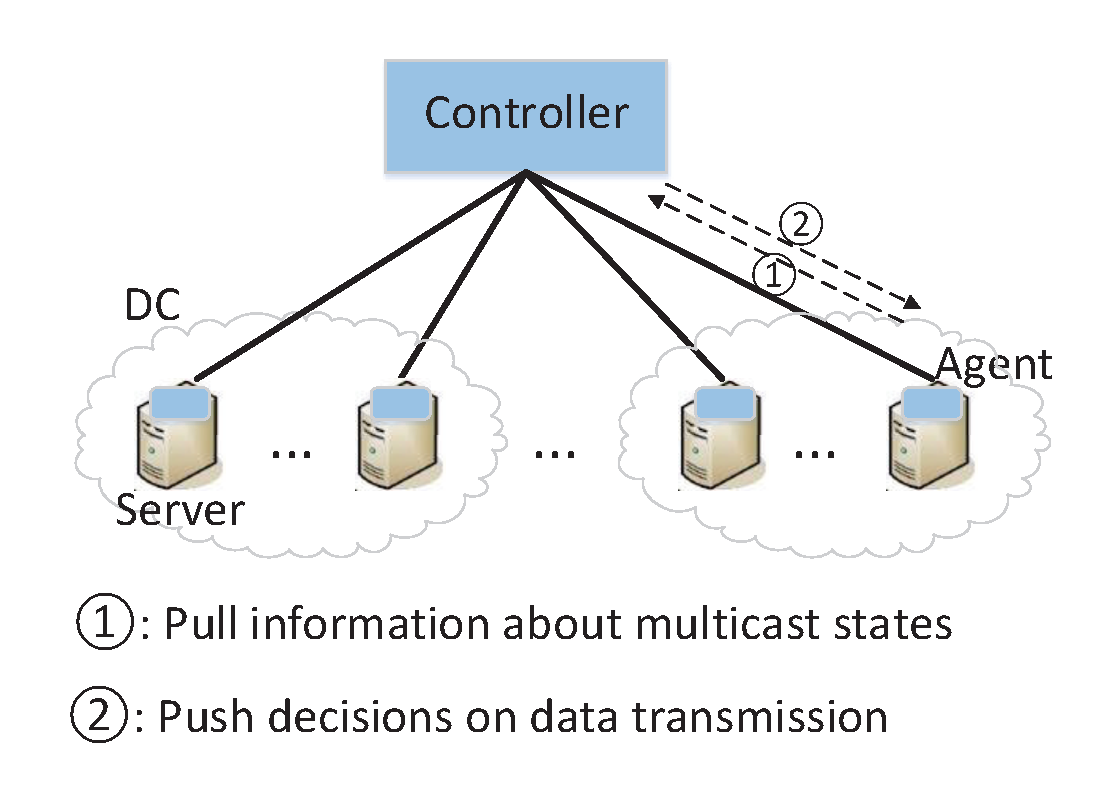
\includegraphics[width=2in]{images/framework.eps}
  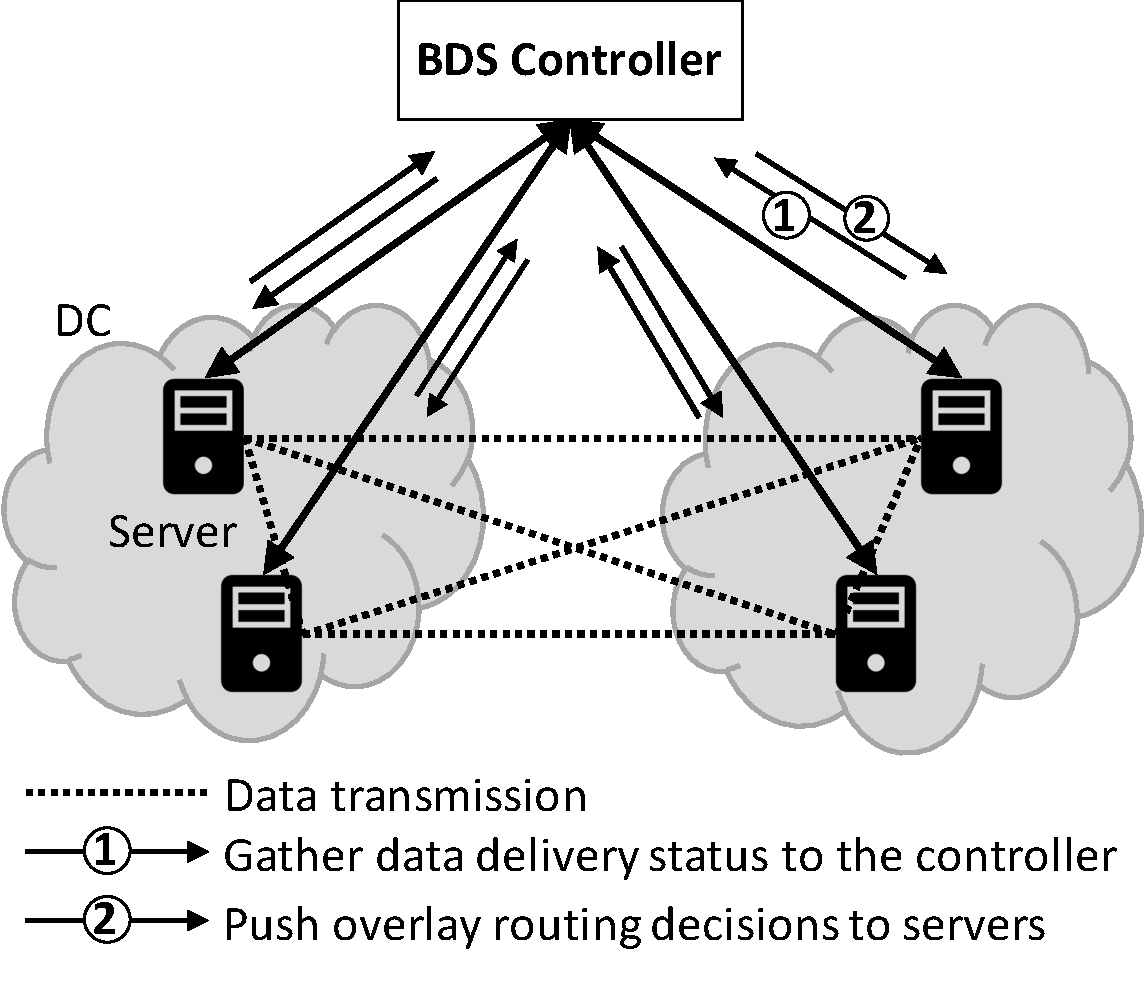
\includegraphics[width=2.3in]{images/framework-new.pdf}
    \vspace{-0.2cm}
  \tightcaption{The centralized design of \name.}
  \label{fig:framework}
\vspace{-0.4cm}
\end{figure}

%\mypara{Centralized design}
%Specifically, the controller schedules data transfers, make the path selection and bandwidth allocation for each transfer in each scheduling period.
%\mypara{Design philosophy}

\name's centralized design is driven by several empirical observations:
\begin{packedenumerate}

\item {\em Large decision space:}
The sheer numbers of inter-DC overlay paths
(which grow exponentially with more servers acting as overlay nodes)
make it difficult for servers to explore all available overlay
paths based only on local measurements.
Instead, we could significantly improve overlay multicast
performance by maintaining a global view of data delivery
status of all servers and dynamically balance
the availability of
various data blocks, which
is critical to achieving near-optimal performance
(\Section\ref{subsec:logic:scheduling}).

\item {\em Large data size:}
Unlike latency-sensitive traffic
(e.g., online partition-aggregation) which lasts on timescales
of several to 10s of milliseconds, inter-DC multicasts are large in volume and
last on much coarser timescales.
%Thus, being highly responsive to transient network dynamics is a necessary concern.
%In this context, the tradeoff between a centralized design and a decentralized one is that centralized control essentially trades real-time responsiveness to network dynamics for closer-to-optimal control decisions driven by a global view of data delivery. Here,
Therefore, \name can tolerate a short delay (of a few seconds) to query a
centralized controller, which maintains a global view of data delivery
and could make optimal decisions.

\item {\em Strict traffic isolation:}
As observed in \Section\ref{subsec:motivation:baseline},
it is vital that inter-DC
multicasts avoid hotspots and excessive bandwidth usage that can increase the latency of delay-sensitive traffic,
but it is difficult to prevent such situations
without any coordination across overlay servers.
In contrast, it is practical
to determine the bandwidth allocation and periodically update it
to all servers in a centralized fashion (\Section\ref{sec:system}).

\item {\em Lower engineering complexity:}
Conceptually, the centralized architecture moves the control complexity to
the centralized controller, making \name amenable to a simpler implementation,
where the control logic running locally in each server can be stateless and
triggered only on arrivals of new data units or control messages.

\end{packedenumerate}

%\mypara{Fast and near-optimal decision-making}
\mypara{The key to realizing centralized control}
In essence, \name trades updating decisions on slightly coarse timescales
for the potential of making optimal decisions in a centralized
fashion.
Thus, the key to striking such a favorable balance is a
near-optimal and efficient overlay routing
algorithm that can be updated on near-realtime timescales.
At a first glance, this is indeed intractable:
the centralized overlay routing algorithm must pick the next hops
from $10^4$s of servers for $10^5$s of blocks, a scale that could
grow exponentially when we consider all possible
overlay paths that go through these servers and finer-grained block partitions.
Using standard routing formulation and solver, it could be completely unrealistic to make optimal solutions by exploring such a large decision space \Section\ref{subsubsec:evaluation:depth}.
%\jc{please add a sentence on how slow it could be with some standard routing formulation and solver}
%It is unclear how this problem can be solved even with limited approximation, which was partly why \company has been lukewarm about a centralized control architecture, despite its potential benefits.
The next section will present how \name addresses this challenge.

%The key technical challenge here is how to make optimal overlay scheduling and routing decisions at the scale tens of thousands of objects and tens of thousands of servers in near real time. To achieve desirable performance in a multicast overlay network, fully exploiting all the available overlay paths is essential, but it is untenable to go through all the potential servers and exponentially more paths by traditional approaches.

%\begin{itemize}
%
%\item Idea \#1: Fully centralized control
%
%\item Idea \#2: Dynamic bandwidth separation: separating background bulk data transfer from latency-sensitive traffic
%
%\item These ideas introduces performance costs (not real time, potentially low link utilization) are outweighed by benefits (not real time, potentially low link utilization)
%
%\item Design philosophy: the costs are outweighed by the benefits. (1) bulk data transfer can tolerate updates at coarse timescales. (2) the aggregation of latency-sensitive data is stable on timescales of several seconds. (3) the resulting system is amenable to simpler implementation.
%
%\item Key technical challenge: how to make optimal overlay scheduling and routing decisions at the scale tens of thousands of objects and tens of thousands of servers in near real time.
%
%\end{itemize}





%\section{Near-Optimal and Efficient Decision-Making Logic}
\label{sec:logic}

At a high level, \name optimizes the data distribution performance by splitting data into fine-grained blocks so as to exploiting all available server-level overlay paths, and possible reordering of blocks to speed up the process.
In a general case, it is indeed intractable to solve the problem in near real-time, but \name can find a near-optimal solution for our problem scale in several seconds by using applying two approximations: (1) separating the problem of data scheduling and overlay routing, and (2) using standard linear-programming relaxation to solve them efficiently.

%\jc{In general, please avoid use of big formulations (like eq 5-10 on p6). May strike a negative impression in nsdi submissions}

\subsection{Problem formulation}
\label{subsec:logic:formulation}

\begin{table}[t]
\begin{center}
%\resizebox{\textwidth/2}{!}{
%\begin{tabular}{p{2cm}<{\centering}|p{2cm}<{\centering}}
\begin{tabular}{| c | l|}
\hline
 \rowcolor[gray]{0.9}
\textbf{Variables} & \textbf{Meaning} \\
\hline \hline
\textit{$\mathbb{A}$} & Set of all $(s, d)$ pair\\
\hline
\textit{$\mathbb{B}$} & Set of blocks of all tasks\\
\hline
\textit{$B_{i,j}$} & Block $i$ in Task $j$\\
\hline
\textit{$c(l_{u,v})$} & Capacity of link $l_{u,v}$\\
\hline
\textit{$Path(s,d)$} & Set of all potential paths in $\mathbb{A}$\\
\hline
\textit{$f_{B_{i,j},p_\lambda}$} & Allocated bandwidth for $B_{i,j}$ on path $p_\lambda$\\
\hline
\textit{$I_{B_{i,j},p_\lambda}$} & 0 or 1: whether $p_\lambda$ is selected for $B_{i,j}$\\
\hline
\end{tabular}
%}
\end{center}
\caption{Variables in \name.}
\label{table:para}
\end{table}

The data distribution problem over inter-DC WANs is defined as follows: We are given one data source DC $S$ and sets of destinations DC $D=\{d_i\}$ in an overlay network, what's the optimal transmission strategy with shortest completion time under a serious of constraints. To formulate this problem and design the decision-making logic for the centralized controller, we should first clarify the following aspects (Table \ref{table:para} summarizes some key variables used in \name):

(1) \textbf{Input.} The number of destination DCs: $m$, the size of data file: $\mathbb{S}$, the set of source and destination pairs: $S=\{(S,d_i)\}, 1\leq i\leq m$ (we name the transmission of data file between $(S,d_i)$ as a ``task'' $T_j$), potential paths between $S$ and $d_i$: $p(S,d_i)$ that consists of multiple links, link capacity of $l_{u,v}$: $c(l_{u,v})$, the upload/download rate of server $n$: $R_{up}(n)/R_{down}(n)$.

(2) \textbf{Output.} The transmission order of blocks on server $s_i$: $\overrightarrow{o}(s_i)$ (we split one task into multiple ``blocks'' because a task is always too large to be transferred in one connection), the optimal source server for the $i$th block of $T_j$ ($B_{i,j}$): $s_{B_{i,j}}^*$, the optimal path for the block: $p_{B_{i,j}}^*$, and the optimal allocated bandwidth on this path: $f^*_{B_{i,j},p_{B_{i,j}}^*}$.

(3) \textbf{Constraints.} The link capacity constraint takes effect on any arbitrary link $l_{u,v}$: the summed allocated bandwidth on this path should be no more than its capacity $c(l_{u,v})$. The path capacity constraint takes effect on path $p_\lambda$: the available capacity $c(p_\lambda)$ should be no more than the minimum capacity of the consisting links. The data size constraint takes effect on blocks: the sum of allocated bandwidth should be no less than its size. The bandwidth constraint defines the allocated bandwidth for $B_{i,j}$ on $p_\lambda$: $f^*_{B_{i,j},p_{B_{i,j}}}$ should be no more than the minimum of the following three parameters: path capacity $c(p_\lambda)$, the upload rate of source node $R_{up}(s)$ and the download rate of destination node $R_{down}(d)$.

(4) \textbf{Objective function.} To speed up the bulk data distribution, \name aims at maximizing the allocated weighted bandwidth for all the blocks over all the paths.

The problem can be formulated precisely according to the above definitions only when the network is static and all the conditions stay unchanged during the whole transmission period. However, it is impractical to make such assumptions because bulk data transfer and constantly changing online traffic co-exists in the network and the design choice of \name is to make dynamic bandwidth separation. Therefore, \name should react to the changing network conditions by monitoring residual bandwidth and re-configured the above formulation (By default, \name tries to update network information and resolve the problem every 3 seconds). Unfortunately, the origin problem becomes considerably complex and hard to solve when making re-formulation, because there will be multiple optional data sources for any arbitrary task. Thus, the searching space grows exponentially and it becomes impossible to find out the optimal transmission. To make it solvable, \name decouples the problem into two parts and tries to find the optimal solutions for each procedure.

\subsection{Separation scheduling and routing}
\label{subsec:logic:separation}

The key insight underlying the above re-formulated problem is the separation of data scheduling and overlay routing, in other words, the data scheduling procedure aims at finding out a subset of blocks that should be transferred first, and only the blocks in this subset should be considered in the following routing process, i.e., outputting the block transmission order $\overrightarrow{o}(s_i)$ ; the overlay routing procedure aims at make optimal routing strategies (assign $s_{B_{i,j}}^*$, $p_{B_{i,j}}^*$ and $f^*_{B_{i,j},p_{B_{i,j}}^*}$) for all selected blocks $B_{i,j}$ in the overlay network.

There are two main benefits of this separation. The first one is to reduce the computational complexity on the centralized controller side. The objective of the separated scheduling stage is to select a subset of blocks, and only these selected blocks will be routed and transferred in the following routing stage. So the separated data scheduling could avoid exploring unnecessary searching spaces for those unselected blocks. The second benefit is to speed up the overall data distribution. This advantage comes from the customized block selection scheme that picks out a specific subset of blocks so as to reduce the overall completion time.

To avoid introducing degradation by the separation to the origin problem, we should make sure that the optimal results does not exist in the ignored searching spaces by the subset selection. In other words, the data scheduling procedure should retain the optimal results although reducing the searching scope. In this way, the optimal routing results in the overlay routing procedure is thus equal to the optimal solution to the origin problem.

\subsection{Scheduling}
\label{subsec:logic:scheduling}

The data scheduling procedure tries to reduce the exploration space while still retaining the potential optimal results. \name achieves this by by selecting a subset of blocks that should be transferred first, i.e., the output of this procedure is the block transmission order $\overrightarrow{o}(s_i)$ for all the servers $s_i$, which is also the input of the next routing procedure.

Assume the origin bulk data in the source DC is split into $n$ blocks, and there are $2m$ DCs in the WAN. Different scheduling strategies will select different block subsets and lead to different intermediate transmission states, finally resulting in different completion time. Take two intermediate states as examples: 1) All of the $n$ blocks has $k$ duplicates; 2) Some of these $n$ blocks have $k1$ $(k1<k)$ duplicates and other blocks have $k2$ $(k2>k)$ duplicates. Let $t_1$ denote the completion time of case 1 and $t_2$ denote that of case 2, we have: $t_2 > t_1$. (See Appendix for the proof)

So in the data scheduling stage, \name will firstly pick out the subset of blocks with the least downloaded duplicates, so as to reduce the overall completion time.

For efficient selection, \name keeps a counter $c_i$ in the controller for each block and updates it once receiving finish notifications from receivers. The scheduling stage always gives priority to the smallest $c_i$. For efficient processing, \name keeps all the counters $c_i$ in a doubly linked list in an ascending order of their values. For each download, the controller selects the top item in the list (the smallest value) to be downloaded. The controller listens and serves an HTTP port, once receiving a transmission completion signal from receivers, it updates the corresponding block's counter value and adjusts its position in the linked list for further processing.

\subsection{Routing}
\label{subsec:logic:routing}

In the overlay routing stage, \name routes and transfers blocks according to $\overrightarrow{o}(s_i)$, the output of data scheduling stage, and then tries to make optimal routing strategy (assign $s_{B_{i,j}}^*$, $p_{B_{i,j}}^*$ and $f^*_{B_{i,j},p_{B_{i,j}}^*}$) for each block $B_{i,j}$.

To speed up data distribution, \name aims at maximizing the allocated weighted bandwidth for all the selected blocks, so the formulation of the objective can be described as:

\begin{equation}
\centering
max \quad \displaystyle{\sum_{(s,d)\in \mathbb{A}}} \displaystyle{\sum_{B_{i,j} \in \mathbb{B}}} \displaystyle{\sum_{p_{\lambda}\in Path(s,d)}} w(B_{i,j})\cdot f_{B_{i,j},p_\lambda} \cdot I_{B_{i,j},p_\lambda}
\end{equation}
where $w(B_{i,j}) = \frac{pr_j}{2^{D_j-t}}$ is the weight of $B_{i,j}$, similar to \cite{zhang2015guaranteeing}, $pr_j$ is the priority of Task $j$, $D_j$ is the deadline and $t$ is the current time, so $2^{D_j-t}$ could represent the urgency. $I_{B_{i,j},p_\lambda}$ denotes whether $p_\lambda$ is selected for $B_{i,j}$. Note that there are multiple potential data sources for each block in the multicast overlay network, so the objective of routing is to select the most efficient data source and assign intermediate paths to all blocks, and then calculate the bandwidth allocation on those selected paths.

The mentioned three constraints can then be formulated as follows:

Link capacity constraint:
\begin{equation}
\begin{split}
c(p_\lambda) \geq & \displaystyle{\sum_{(s,d)\in \mathbb{A}}} \displaystyle{\sum_{B_{i,j} \in \mathbb{B}}} f_{B_{i,j},p_\lambda} \cdot I_{B_{i,j},p_\lambda}\\
& \forall p_\lambda \in Path(s,d) \label{st:capacity}
\end{split}
\end{equation}

Data size constraint:
\begin{equation}
\begin{split}
\mathbb{S}(B_{i,j}) \leq & \displaystyle{\sum_{(s,d)\in \mathbb{A}}} \displaystyle{\sum_{p_{\lambda}\in Path(s,d)}} f_{B_{i,j},p_\lambda} \cdot I_{B_{i,j},p_\lambda} \cdot \Delta T\\
& \forall B_{i,j} \in \mathbb{B} \label{st:size}\\
\end{split}
\end{equation}

Bandwidth constraint:
\begin{equation}
\begin{split}
f_{B_{i,j},p_\lambda} \leq & min \{c(p_\lambda),R_{up}(s),R_{down}(d)\}\\
& \forall p_\lambda \in Path(s,d) \label{st:bottleneck}
\end{split}
\end{equation}

Besides, there is another limitation on path selection: $\displaystyle{\sum_{p_\lambda \in Path(s,d)}} I_{B_{i,j},p_\lambda} = 1$, which means only one path will be chosen for a particular block.

The integer program (IP) is a multi-commodity flow algorithm which is known to be NP-complete \cite{garg1997primal} due to the fact that they are integer flows, and there is no known algorithm to find an optimal solution. To make this problem solvable, we look into it from a different perspective. As the size of a task is dozens of TBs to PBs, while each block is just about several MBs, we can approximate tasks although they are infinitesimally split and can be transferred to a set of possible paths between the source DC and the destination DC. So it is possible to solve this IP problem by a linear programming (LP) relaxation \cite{garg2007faster,reed2012traffic}, and the relaxed problem aims at transferring a fraction of each transmission. However, the number of blocks will thus grow considerably large when splitting tasks infinitesimally, and this will lead to intolerable computing time on the controller side. There are two coping strategies on this problem: on one hand, \name has a merge scheme before each transmission cycle, and this step merges blocks with the same (s,d) pair into one subtask so as to reduce task number; on the other hand, \name adopts the improved fully polynomial-time approximation schemes (FPTAS) by Fleischer \cite{fleischer2000approximating} to work out an $\epsilon$-optimal solution with $\alpha' \geq \alpha_\epsilon \geq \alpha'(1-\epsilon)^{-3}$. This algorithm optimizes the dual problem of the relaxed LP problem by proceeding in phases and iterations (see Appendix for the proof of near optimality of \name).

\section{Near-Optimal and Efficient Decision-Making Logic}
\label{sec:logic}

At the core of \name is a centralized decision-making
algorithm that periodically updates near-optimal overlay
routing decisions at scale  in near real-time.
% (e.g., $10^4$s of overlay paths and $10^5$s of data blocks).
%At a high level, to optimize inter-DC data multicast, \name fully
%exploits application-level overlay paths by splitting data into
%small blocks and periodically selecting the overlay paths to send
%each data block.
%While achieving this may be indeed intractable due to the
%sheer numbers of available overlay paths and data blocks,
\name strikes a favorable tradeoff between solution optimality
and fast update by
{\em decoupling} the problem into two steps (\Section\ref{subsec:logic:separation}):
overlay scheduling, i.e., which data blocks to be sent
(\Section\ref{subsec:logic:scheduling});
and routing, i.e., which path to send each data block
(\Section\ref{subsec:logic:routing}), each of which
can be solved efficiently and near-optimally with proved guarantees
(\Section\ref{subsec:logic:scheduling},~\ref{subsec:logic:routing}).

%At a high level, \name optimizes the data distribution performance by splitting data into fine-grained blocks so as to exploiting all available server-level overlay paths, and possible reordering of blocks to speed up the process.
%In a general case, it is indeed intractable to solve the problem in near real-time, but \name can find a near-optimal solution for our problem scale in several seconds by using applying two approximations: (1) separating the problem of data scheduling and overlay routing, and (2) using standard linear-programming relaxation to solve them efficiently.

%\jc{In general, please avoid use of big formulations (like eq 5-10 on p6). May strike a negative impression in nsdi submissions}

\subsection{Basic formulation of overlay control}
\label{subsec:logic:formulation}

%\begin{table}[t]
%\begin{center}
%%\resizebox{\textwidth/2}{!}{
%%\begin{tabular}{p{2cm}<{\centering}|p{2cm}<{\centering}}
%\begin{tabular}{| c | l|}
%\hline
% \rowcolor[gray]{0.9}
%\textbf{Variables} & \textbf{Meaning} \\
%\hline \hline
%\textit{$\mathbb{A}$} & Set of all $(s, d)$ pair\\
%\hline
%\textit{$\mathbb{B}$} & Set of blocks of all tasks\\
%\hline
%\textit{$B_{i,j}$} & Block $i$ in Task $j$\\
%\hline
%\textit{$c(l_{u,v})$} & Capacity of link $l_{u,v}$\\
%\hline
%\textit{$Path(s,d)$} & Set of all potential paths in $\mathbb{A}$\\
%\hline
%\textit{$f_{B_{i,j},p_\lambda}$} & Allocated bandwidth for $B_{i,j}$ on path $p_\lambda$\\
%\hline
%\textit{$I_{B_{i,j},p_\lambda}$} & 0 or 1: whether $p_\lambda$ is selected for $B_{i,j}$\\
%\hline
%\end{tabular}
%%}
%\end{center}
%\caption{Variables in \name.}
%\label{table:para}
%\end{table}

\begin{table}[t]
\begin{center}
\resizebox{3in}{!}{
%\begin{tabular}{p{2cm}<{\centering}|p{2cm}<{\centering}}
\begin{tabular}{| c | l|}
\hline
 \rowcolor[gray]{0.9}
\textbf{Variables} & \textbf{Meaning} \\
\hline \hline
\textit{$\mathbb{A}$} & Set of all source and destination (s,d) pairs\\
\hline
\textit{$\mathbb{B}$} & Set of blocks of all tasks\\
\hline
\textit{$B_{i,j}$} & Block $i$ in Task $j$\\
\hline
\textit{$c(l_{u,v})$} & Capacity of link $l_{u,v}$\\
\hline
\textit{$R_{up}(n)/R_{down}(n)$} & Upload/download rate limit of server $n$\\
\hline
\textit{$Path(s,d)$} & Set of all possible paths in $\mathbb{A}$\\
\hline
\textit{$s_{B_{i,j}}$} & Data source of $B_{i,j}$\\
\hline
\textit{$f_{B_{i,j},p_\lambda}$} & Transmission rate of $B_{i,j}$ on path $p_\lambda$\\
\hline
\textit{$I_{B_{i,j},p_\lambda}$} & 0 or 1: whether $p_\lambda$ is selected for $B_{i,j}$\\
\hline
%\textit{$f(l_{u,v}$)} & The allocated transmission rate on link $l_{u,v}$\\
%\hline
\end{tabular}
}
\end{center}
\vspace{-0.4cm}
\tightcaption{Notations in \name.}
\label{table:para}
\end{table}

\mypara{Under fixed network capacity}
We start with the basic formulation of the overlay control under the assumption of fixed network capacity and fixed demand of multicast requests. We will later extend it to dynamic network performance and traffic demands. With the key variables and parameters summarized in the Table \ref{table:para}, the problem of multicast overlay routing can be formulated as follows:
%The data distribution problem over inter-DC WANs is defined as follows: We are given one data source DC $S$ and sets of destinations DC $D=\{d_i\}$ in an overlay network, what's the optimal transmission strategy with shortest completion time under a serious of constraints. To formulate this problem and design the decision-making logic for the centralized controller, we should first clarify the following aspects (Table \ref{table:para} summarizes some key variables used in \name):

%\jc{Notions are too complicated. Please simplify. 4.1 should be at most 1/3 pg.}

\noindent(1) {\em Input.}% \jc{the formulation only consider one multicast request? No, multiple.}
%One source DC, sets of destination DCs,
%network topology,
%server upload (and download) rate limit,
%link capacity.
Each multicast transmission, referred to as a {\em task} $T$, is defined
by a source DC, a set of destination DCs, and a data file chopped into
a list of fixed-sized data
{\em blocks}\footnote{Splitting data into fine-grained blocks enables
parallel transfer along
multiple overlay paths to increase throughput, though too small data blocks
increases computational overhead of the routing algorithm.
In practice, we found 2MB is a good tradeoff
(\Section\ref{subsec:evaluation:benchmarks:parameters})}.
%the block size is 2MB, for efficient transmission and acceptable calculation overhead)
The $i$th block of the $j$th task is denoted as $B_{i,j}$.
Besides traffic demand, the inputs also include link capacity $c(l_{u,v})$ and
server upload (and download) rate limit $R_{up}(n)/R_{down}(n)$. %\jc{what're the notions of toplogy, bandwidth? aren't link capacity and rate limit the same? Not the same, link capacity is the attribute of links and rate limit is the attribute of servers.}

\noindent(2) {\em Output.} A four tuple for each server: $\langle \overrightarrow{o_\mathbb{B}}, s_{\mathbb{B}}^*, p_{\lambda}^*, f^*_{\mathbb{B},p_{\lambda}^*} \rangle$, which denotes the block transmission sequence, the optimal source, overlay path for each block, and the optimal allocated bandwidth on this path, respectively. %\jc{what the hell is B?!, and where's the server notation?}

\noindent(3) {\em Constraints.}
The formulation is subject to constraints similar to those of maximum concurrent flow (MCF) problem~\cite{garg2007faster,reed2012traffic}.\jc{you can tighten the space between equations and texts, if you need space}
%There are four constraints on link capacity, data size, bandwidth allocation and path selection:

%The mentioned three constraints can then be formulated as follows:
\begin{packeditemize}
\item Link capacity. The summed allocated bandwidth on this path should be no more than its capacity $c(p_\lambda)$, where $f_{B_{i,j},p_\lambda}$ is the allocated bandwidth for $B_{i,j}$ on path $p_\lambda$ and $I_{B_{i,j},p_\lambda}$ denotes whether $p_\lambda$ is selected for $B_{i,j}$.
\begin{equation}
%\begin{split}
c(p_\lambda) \geq  \displaystyle{\sum_{(s,d)\in \mathbb{A}}} \displaystyle{\sum_{B_{i,j} \in \mathbb{B}}} f_{B_{i,j},p_\lambda} \cdot I_{B_{i,j},p_\lambda}\\
%& \forall p_\lambda \in Path(s,d) \label{st:capacity}
%\end{split}
\end{equation}

\item Data size. The sum of allocated bandwidth should be no less than its size $\mathbb{S}(B_{i,j})$.
\begin{equation}
%\begin{split}
\mathbb{S}(B_{i,j}) \leq  \displaystyle{\sum_{(s,d)\in \mathbb{A}}} \displaystyle{\sum_{p_{\lambda}\in Path(s,d)}} f_{B_{i,j},p_\lambda} \cdot I_{B_{i,j},p_\lambda} \cdot \Delta T\\
%& \forall B_{i,j} \in \mathbb{B} \label{st:size}\\
%\end{split}
\end{equation}

\item Bandwidth allocation. The allocated bandwidth on path $p_\lambda$ should be the minimum of three parameters: the capacity $c(p_\lambda)$, source server upload rate $R_{up}(s)$, and destination server download rate $R_{down}(d)$.
\begin{equation}
%\begin{split}
f_{B_{i,j},p_\lambda} \leq  min \{c(p_\lambda),R_{up}(s),R_{down}(d)\}\\
%& \forall p_\lambda \in Path(s,d) \label{st:bottleneck}
%\end{split}
\end{equation}

\item Path selection. Only one path will be chosen for a particular block.
$\displaystyle{\sum_{p_\lambda \in Path(s,d)}} I_{B_{i,j},p_\lambda} = 1$
\end{packeditemize}
%\jc{maybe it's better in math after all. please write
%it in math and add comments in the end to describe the
%meaning}
%%The link capacity constraint takes effect on any arbitrary link $l_{u,v}$:
%for each link $l_{u,v}$,
%the summed allocated bandwidth on this path should be
%no more than its capacity $c(l_{u,v})$,
%and for each path $p_\lambda$, the available capacity
%$c(p_\lambda)$ should be no more than the minimum
%capacity of the consisting links.
%%The path capacity constraint takes effect on path $p_\lambda$: the available capacity $c(p_\lambda)$ should be no more than the minimum capacity of the consisting links.
%The data size constraint takes effect on blocks: the sum of allocated bandwidth should be no less than its size. The bandwidth constraint defines the allocated bandwidth for $B_{i,j}$ on $p_\lambda$: $f^*_{B_{i,j},p_{B_{i,j}}}$ should be no more than the minimum of the following three parameters: path capacity $c(p_\lambda)$, the upload rate of source node $R_{up}(s)$ and the download rate of destination node $R_{down}(d)$.

\noindent(4) {\em Objective.} To speed up the bulk data distribution, \name aims at maximizing the sum of allocated bandwidth for all the blocks over all the paths.

\begin{equation}
\centering
max \quad \displaystyle{\sum_{(s,d)\in \mathbb{A}}} \displaystyle{\sum_{B_{i,j} \in \mathbb{B}}} \displaystyle{\sum_{p_{\lambda}\in Path(s,d)}} w(B_{i,j})\cdot f_{B_{i,j},p_\lambda} \cdot I_{B_{i,j},p_\lambda}
\label{equation:objective}
\end{equation}
where $w(B_{i,j}) = \frac{pr_j}{2^{D_j-t}}$ is the weight of $B_{i,j}$, similar to \cite{zhang2015guarantee}, $pr_j$ is the priority of Task $j$, $D_j$ is the deadline and $t$ is the current time.

\mypara{Dynamic updates}
Since any change in network performance or arrival of
new requests may alter the optimal overlay
routing decisions,
%The problem can be formulated precisely according to the above definitions only when the network is static and all the conditions stay unchanged during the whole transmission period. However, it is impractical to make such assumptions because bulk data transfer and constantly changing online traffic co-exists in the network and the design choice of \name is to make dynamic bandwidth separation. Therefore,
\name updates the solutions to the above formulation every cycle of 3 seconds, which is empirically sufficient to achieve near-optimal performance (\Section\ref{subsubsec:evaluation:depth}). Unfortunately, the origin formulation is intractable in practice, because the computational overhead grows exponentially with more potential sources, paths, and data blocks.

%To make it tractable, \name decouples the problem into two steps and tries to find the optimal solution for each step.

%\jc{a missing piece is how large each block is, and why. }

\subsection{Decoupling scheduling and routing}
\label{subsec:logic:separation}

At a high level, the key insight of \name to update the overlay control problem is
to decouple the aforementioned formulation into two steps:
a {\em scheduling} step which selects a subset of blocks to be transferred
($\overrightarrow{o_\mathbb{B}}$), followed by a subsequent {\em routing}
step which determines the residual three tuples: $\langle s_{\mathbb{B}}^*, p_{\lambda}^*, f^*_{\mathbb{B},p_{\lambda}^*} \rangle$. %routing paths ($p_{\lambda}^*$) and the allocated bandwidth ($f^*_{\mathbb{B},p_{\lambda}^*}$) of these blocks.

On one hand, such decoupling significantly reduces the computational overhead of the centralized controller. As the scheduling step selects a subset of blocks and only these selected blocks will be considered in the following routing step, the searching spaces are thus significantly reduced, speeding up the execution of the centralized algorithm.

On the other hand, such decoupling is near-optimal. In the origin formulation, the optimal solution is to decide the optimal block transmission order $\overrightarrow{o_\mathbb{B}}$ for all blocks, while such decoupling converts this optimal solution into an equivalent one, i.e., to decide the optimal order to transmit the selected blocks in each scheduling cycle (so as to enforce network dynamic updates). Thus, the decoupling introduces little degradation as long as \name could find the optimal solutions for both scheduling and routing steps in each cycle.

%In the existing hybrid CDN and P2P architecture \cite{yin2009design} or centralized P2P scheme \cite{lee2003centralized}, there are also centralized servers with global information, but those servers are used for specific tasks (like system bootstrapping and maintaining global index) \cite{androutsellis2004survey}. While the centralized controller of \name faces more challenges in terms of real-time computing. The above mentioned decoupling could not only sense the changing network conditions, but also reduce the calculation scale of the centralized algorithm running on the controller.
%uses the global information to decouple scheduling and routing without introducing degradation.\jc{put the last sentence after the benefits. also, i don't get the point of this sentence.}
%, i.e., outputting the block transmission order $\overrightarrow{o}(s_i)$ ; the overlay routing procedure aims at make optimal routing strategies (assign $s_{B_{i,j}}^*$, $p_{B_{i,j}}^*$ and $f^*_{B_{i,j},p_{B_{i,j}}^*}$) for all selected blocks $B_{i,j}$ in the overlay network.
%There are two main benefits of this separation.
%\begin{packedenumerate}
%\item It reduces the computational complexity on the centralized controller side. The objective of the separated scheduling stage is to select a subset of blocks, and only these selected blocks will be routed and transferred in the following routing stage. So the separated data scheduling could avoid exploring unnecessary searching spaces for those unselected blocks.
%\item It speeds up the overall data distribution. This advantage comes from the customized block selection scheme that picks out a specific subset of blocks so as to reduce the overall completion time.
%\jc{why this is a benefit of decoupling? seems an advantage of centralized control?}
%\end{packedenumerate}
%
%\mypara{Why such decoupling is near-optimal}
%The optimal solution for the origin bulk data transfer problem is to decide the optimal order $\overrightarrow{o}(s_i)$ to transmit block for all servers, while such decoupling converts the origin problem into an equivalent one: to decide the optimal order to transmit the selected blocks in each scheduling cycle (so as to enforce network dynamic updates). Thus, the decoupling introduces no degradation as long as \name finds the optimal solutions for both of the scheduling and routing procedures.
%
%\jc{how about the following flow:
%para1: what the decoupling means; \\
%para2: why it saves costs; \\
%para3: why it could be near-optimal;\\
%para4: why people haven't thought about this or why our solution is unique}

%\jc{still unclear why this decoupling is efficient and near optimal}

%\jc{you had a table to describe all the math notations. why it's missing? it's important! im also confused what's difference between source and copy?}

\subsection{Scheduling}
\label{subsec:logic:scheduling}

The scheduling step
%tries to reduce searching space by selecting
selects the subset of blocks to be transferred in each cycle and
outputs the transmission order $\overrightarrow{o_\mathbb{B}}$. As analyzed before, the centralized overlay routing algorithm should pick the data source from $10^4$s of servers for $10^5$s of blocks, and this scale could even grow exponentially when we consider more fine-grained block partitions. Such computational complexity makes it intractable for the controller to explore all the possible paths to make optimal decisions on near-realtime timescales. Therefore, the scheduling step aims at reducing the sheer numbers of potential overlay paths, and thus reduces the searching space of the centralized algorithm.
%\jc{reducing what search space? and why we need to reduce it?}

The key to avoid introducing degradation in this process is to make sure that the optimal result is still retained in the reduced searching space.
%In other words, the optimal result is not in the space that is pruned by scheduling procedure.
%We show that the a simple-yet-efficient way of achieving optimal scheduling result is to maintain same amount of copies of each data block. We will give a full proof of the above statement in Appendix~\ref{??}, but let us  intuitively explain it here.
We claim that {\em the optimal result is yielded from the balance availability of all data blocks}, i.e., all the blocks are duplicated for the same amount of copies. Thus, a simple-yet-efficient way of avoiding degradation when reducing searching space is to balance block availability. We will give a full proof of the above statement in Appendix~\Section\ref{appendix:balance}.
%, but let us intuitively explain it here.
%thus the key concern is to balance the duplication of all blocks. So here \name prunes the searching space that will not result in balanced duplications and selects the least duplicated blocks to transmit first.
%In this way, the optimal result will be retained in the reduced searching space.
%\jc{this is a key statement! please make it more precisely}
%To be specific,
%Assume the origin data in the source DC is split into $n$ blocks, and there are $2m$ destination DCs in the WAN. Different scheduling strategies output different block subsets and lead to different intermediate transmission states, finally resulting in different completion time. Take two intermediate states as examples: 1) All of the $n$ blocks are balanced duplicated (i.e., each with $k$ duplicates); 2) Blocks are imbalanced duplicated (some have $k1$ duplicates and some have $k2$ duplicates, $(k1<k<k2)$). Let $t_1$ denote the completion time of case 1 and $t_2$ denote that of case 2. The proof in Appendix~\Section\ref{appendix:balance} shows $t_1 < t_2$, which proves the above claim.
Therefore, in this scheduling step, \name will firstly pick out the subset of blocks with the least amount of duplicates, to balance the block availability.
%\jc{wtf... this example says nothing. what's the intuition behind balancing duplicates? }

%\jc{isn't it trivial to maintain the counters?}
%For efficient selection, \name keeps a counter $c_i$ in the controller for each block and updates it once receiving finish notifications from receivers. The scheduling stage always gives priority to the smallest $c_i$. For efficient processing, \name keeps all the counters $c_i$ in a doubly linked list in an ascending order of their values. For each download, the controller selects the top item in the list (the smallest value) to be downloaded. The controller listens and serves an HTTP port, once receiving a transmission completion signal from receivers, it updates the corresponding block's counter value and adjusts its position in the linked list for further processing.

\subsection{Routing}
\label{subsec:logic:routing}

With the scheduling step selects the block set to transfer ($\overrightarrow{o_\mathbb{B}}$), the routing step then decides the residual three tuples, $\langle s_{\mathbb{B}}^*, p_{\lambda}^*, f^*_{\mathbb{B},p_{\lambda}^*} \rangle$, for all blocks.% $\mathbb{B}$, the source $s_{\mathbb{B}}^*$, the path $p_{B}^*$, and bandwidth allocation of the path $f^*_{B,p_{B}^*}$.
%In the overlay routing step, \name routes and transfers blocks according to the output of data scheduling step ($\overrightarrow{o_B}$), and then tries to make optimal routing strategy (assign $s_{B}^*$, $p_{B}^*$ and $f^*_{B,p_{B}^*}$) for each block $B$.
%Note that there are multiple potential data sources for each block in the multicast overlay network, so the objective of routing is to pick the most efficient data source and paths before allocating the bandwidths on these selected paths.

With the constraints described in \Section\ref{subsec:logic:formulation}, this formulation in Equation \ref{equation:objective} is an integer multi-commodity flow algorithm which is known to be NP-complete \cite{garg1997primal}.
%, and there is no known algorithm to find an optimal solution. 
To make this problem tractable in practice,
%we look into it from a different perspective. As the size of a task is 10s of TBs to PBs, while each block is just about several MBs,
we assume each data file can be infinitesimally split and transferred simultaneously on a set of possible paths between the source DC and the destination DC.
This approximation closely resembles \name's actual routing step as \name also splits data into tens of thousands of fine-grained data blocks (though not infinitesimally), and it can be solved efficiently by standard linear programming (LP) relaxation commonly used in the MCF problem~\cite{garg2007faster,reed2012traffic}.
The key idea is to transfer at least a fraction $\alpha$ of each task,%\jc{what's a transmission},
%Such MCF problem provides a solution to the original NP-complete problem, although with fractional flows.
and the optimal transmission rate of the relaxed problem is $F^*=\alpha\dot f^*$, where $f^*$ is the optimal transmission rate of the original routing problem.
Therefore, finding the optimal solution to the original problem becomes simply maximing $\alpha$ instead, and this can be solved in polynomial time.
%equivalent to that of the original problem $f^*$ with a relationship given by $F^* / \alpha = f^*$. Thus, the original problem is converted to maximize $\alpha$ and can be solved within polynomial time.

However, when splitting tasks infinitesimally, the number of blocks will grow considerably large and the computing time will be intolerable. \name adopts two coping strategies: on one hand, it merges the blocks with the same source and destination pair into one subtask so as to reduce the calculation scale; on the other hand, it adopts the improved fully polynomial-time approximation schemes (FPTAS) (\cite{fleischer2000approximating}) to optimize the dual problem of the origin problem and works out an $\epsilon$-optimal solution (see Appendix~\Section\ref{appendix:optimality} for the proof of near-optimality of \name).% with $\alpha' \geq \alpha_\epsilon \geq \alpha'(1-\epsilon)^{-3}$. This algorithm optimizes the dual problem of the relaxed LP problem by proceeding in phases and iterations
%\jc{sorry, but i'm totally lost. what's the key idea? is it just a standard LP relaxation?}
\jc{is this the same as ``blocks merging'' in the next section?}


\section{System Design}
\label{sec:system}

This section presents the system design and implemetation of \NEW{\name/\newname.}

\subsection{Centralized control of \name}
\label{subsec:system:centralized}

\begin{figure}[t]
  \centering
  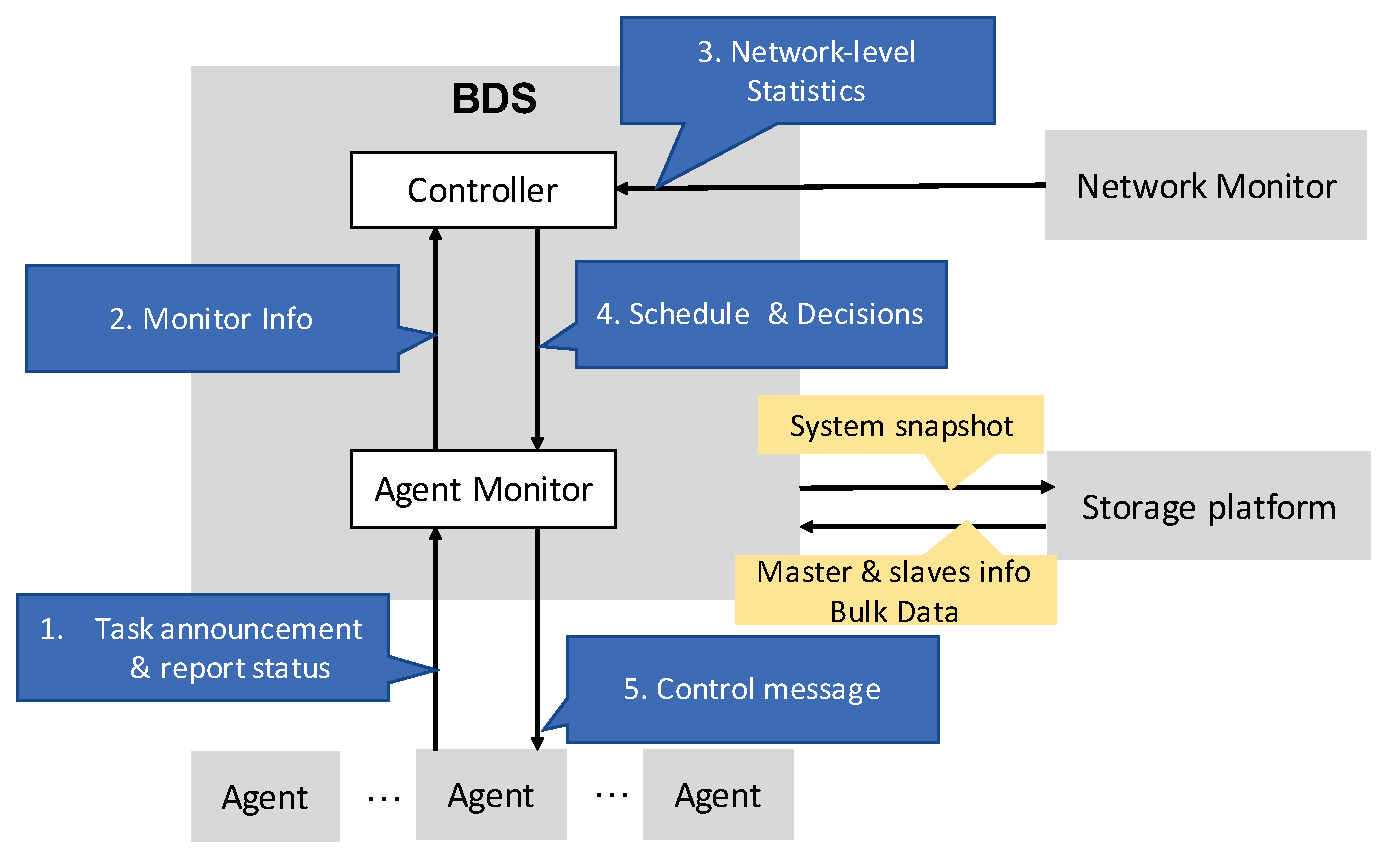
\includegraphics[width=3in]{images/implementation_v4.eps}
  \tightcaption{Interfaces of \name's centralized control.}
% \jc{please add the step of network monitor. see the new text}\jc{where are servers? avoid notions never defined before like "task announcement"}
  \label{fig:implementation}
%\vspace{-0.4cm}
\end{figure}
%\vspace{-15pt}

\name periodically (by default, every three seconds) updates the
routing and scheduling decisions in a centralized fashion.
Figure \ref{fig:implementation} outlines the workflow in each
three-second cycle.
\begin{enumerate}
\item It starts with the {\em Agent}, running local on each server,
checking the local states, including data block delivery status
(which blocks have arrived, and which blocks are outstanding),
server availability, and disk failures, etc.
\item These statistics are then wrapped in a {\em control message},
and sent to the centralized {\em \name Controller} via an efficient
messaging layer called {\em Agent Monitor}.
\item The \name Controller also receives network-level statistics
(the bandwidth consumption by latency-sensitive traffic and the
utilization on each inter-DC link) from a {\em Network Monitor}.
\item On receiving the updates from all Agents and the Network
Monitor, the \name Controller runs the centralized decision-making
algorithm (\Section\ref{sec:logic}) to work out the new scheduling
and routing decisions, and sends the difference between the new
decision and the previous one to the per-server local Agent via
the Agent Monitor messaging layer.
\item Finally, the Agent allocates bandwidth for each data transfer,
and carries out the actual data transfers according the Controller's
routing and scheduling decisions.
\end{enumerate}


\name uses two additional optimizations to make the workflow
more efficient.
\begin{itemize}
\item \emph{Blocks merging}.
To reduce the computational scale and achieve more efficient
transmissions, \name merges the blocks with the same source and
destination into one subtask. Its benefits are two-fold: (1) it
significantly reduces the number of pending blocks in each
scheduling cycle, thus reducing the computational cost of the
centralized decision-making logic; and (2) it reduces the number
of parallel TCP connections between servers, which could
otherwise reduce link utilization and degraded performance.
\item \emph{Non-blocking update}.
To avoid being blocked by the controller's decision-making logic,
each local Agent  keeps the ongoing data transmissions alive while
the Controller runs the centralized decision-making logic.
Similarly, the Controller takes this into account by speculating
the changes in data delivery status while the decisions are being
re-calculated, and using these speculated data delievery status as
the input of the centralized logic.
\end{itemize}

\NEW{
\subsection{Dynamic bandwidth separation of \newname}
\label{subsec:system:separation}

To guarantee dynamic bandwidth separation between inter-DC
bulk-data multicasts and delay-sensitive traffic, \newname Network
Change Monitor detects any changes of the aggregated bandwidth usage of all
latency-sensitive flows on each inter-/intra-DC link, and
dynamically allocates the bandwidth for bulk-data multicast
transfer accordingly. To protect delay-sensitive flows from being negatively
affected by bursty bulk-data transfers, \newname is designed to be sensitive to network changes by using a sliding k in the traffic prediction algorithm. In other words, it puts more importance to sudden increases or decreases when online traffic oscillates (to be sensitive), while refers to history information when online traffic isn't changing much (to be stable).
%set an upper bound K for the EWMA algorithm, k is set to be
%K when there is no change points, and will be reset to 0 once a
%change point is detected, and then gradually increase to K.
%\name uses 80\% link
%utilization as a ``safety threshold'', i.e., the total bandwidth
%consumption of bulk-data transfers cannot exceed 80\% of the link
%capacity on any link, and dynamically decides the sending rate
%of each data transfer.

\newname's dynamic bandwidth separation also takes advantage of the centralized logic of \name. The traditional
techniques (e.g.,~\cite{kumar2015bwe}) that gives higher priority to
online latency-sensitive traffic can still have bandwidth wastage or
performance interference in the presence of dynamic network
environments~\cite{wang2017toward}. \newname, in contrast, dynamically predicts the
bandwidth usage of latency-sensitive applications, and calculates the
residual bandwidth that can be used by inter-DC multicast. Finally, note that \newname optimizes
the application-level overlay, and is thus complementary to
network-layer techniques that improve the WAN performance and
fairness~\cite{chen2012design, kavulya2010analysis, mishra2010towards, reiss2012heterogeneity}.
}

\subsection{Fault tolerance}
\label{subsec:system:fault}
Next we describe how \name/\newname handles the following failures.

\begin{packedenumerate}
\item \emph{Controller failure:} The controller is
replicated~\cite{lamport1998part}: if the master controller fails,
another replica will be elected as the new controller. If all
controller replicas are not available (e.g., a network partition
between DCs and the controllers), the agents running in servers will
fallback to the current decentralized overlay protocol as default to
ensure graceful performance degradation.
\item \emph{Server failure:} If the agent on server is still able to
work, it will report the failure state (e.g., server crash, disk
failure, etc.) to the agent monitor in the next cycle. Otherwise, the
servers that selected this server as data source would report the
unavailability to the agent monitor. In either case, the controller
will remove that server from the potential data sources in the next
cycle.
\item \emph{Network partition between DCs:}
If network partition happens between DCs, the DCs located in the same
partition with the controller will work the same as before, while the
separated DCs will fallback to the decentralized overlay network.
\end{packedenumerate}




%
\subsection{Implementation and Deployment}
\label{sec:deployment}

%\begin{figure}[t]
%  \centering
%  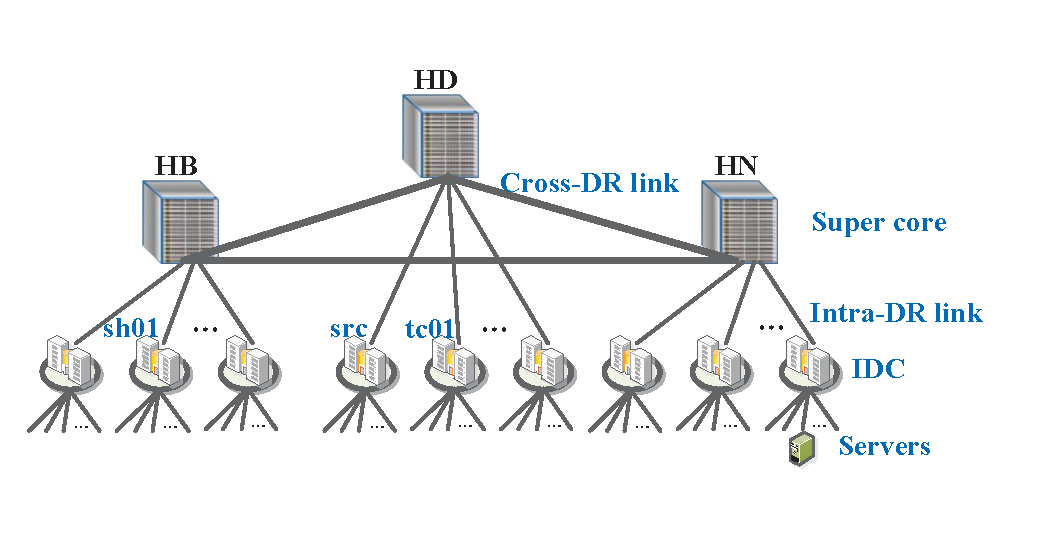
\includegraphics[width=3in]{images/Testbed_v2.eps}
%  \tightcaption{The abstract topology of our intra-net WAN.}
%  \label{fig:topology}
%\vspace{-0.1in}
%\end{figure}
%\vspace{-15pt}

We have deployed \name on \company's DCs, which consist of 67 geo-distributed servers in 10 DCs. Evaluations in the next section are based on this deployment. %The topology is shown as Fig. \ref{fig:topology}.

\name is implemented with 3621 lines of golang code \cite{golang}, and can be fully integrated in \company's DCs. The three duplications of the controller are implemented on three different geo-located servers. The data plane (bulk data transmissions) between controller and agents adopts TCP, and the control plane (decision messages) adopts HTTP. For the specific transmissions, \name uses \emph{wget} to make data transfer and sets particular \emph{wget options} to enforce bandwidth.

This implementation makes no specific requirements on applications, and any application that wants to distribute bulk data just needs to follow three steps: 1. register on \name, initiate the basic information about source DC, destination DCs, all end servers and the bulk data. 2. install agents on the involved end servers, 3. assign the start time of bulk data transmission. Then \name will start the data distribution at the specified time. Such simple implementation also makes \name applicable to other companies' DCs. 	

%\jc{this is oversimplistic. did you make any assumption about the agent? what if a hadoop application wants to use your stuff?}

%\jc{a missing piece is what's application interface. if an application wants to send a file, does it make a function call to your system?}

%\jc{what changes did you make on each server? where was the controller implemented? what's the protocol? how did data transfer happen (wget?)? how was bandwidth enforcement done (wget option)? }



%
%\begin{itemize}
%\item \name consists of \fillme line of \fillme code, and can be fully integrated in \company's DCs.
%
%\item Application interfaces: What information does an application need to announce to \name to initiate a multicast.
%
%\item What's the software platform to implement each component
%
%\item Why \name is also applicable to other DCs?
%
%\end{itemize}


%
%\section{Evaluation}
\label{sec:evaluation}
\begin{figure*}[t]
        \centering
        \begin{subfigure}[b]{0.3\textwidth}
                \centering
                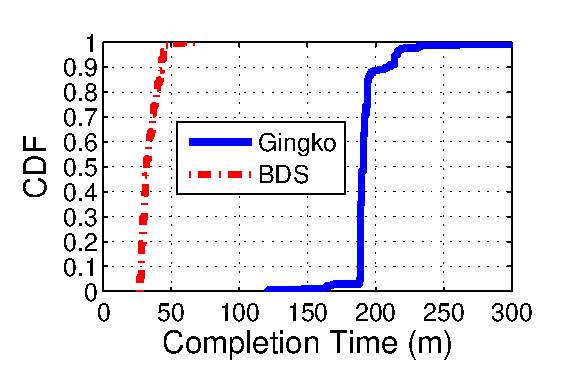
\includegraphics[width=\textwidth]{images/BDSvsAnon_overall_v2.eps}
                \caption{Distribution of completion time.}
                \label{fig:BDSvsAnon:overall}
        \end{subfigure}
        \begin{subfigure}[b]{0.3\textwidth}%@X:\6 PieBridge\simulation\beijing\3 Applications\plot
                \centering
                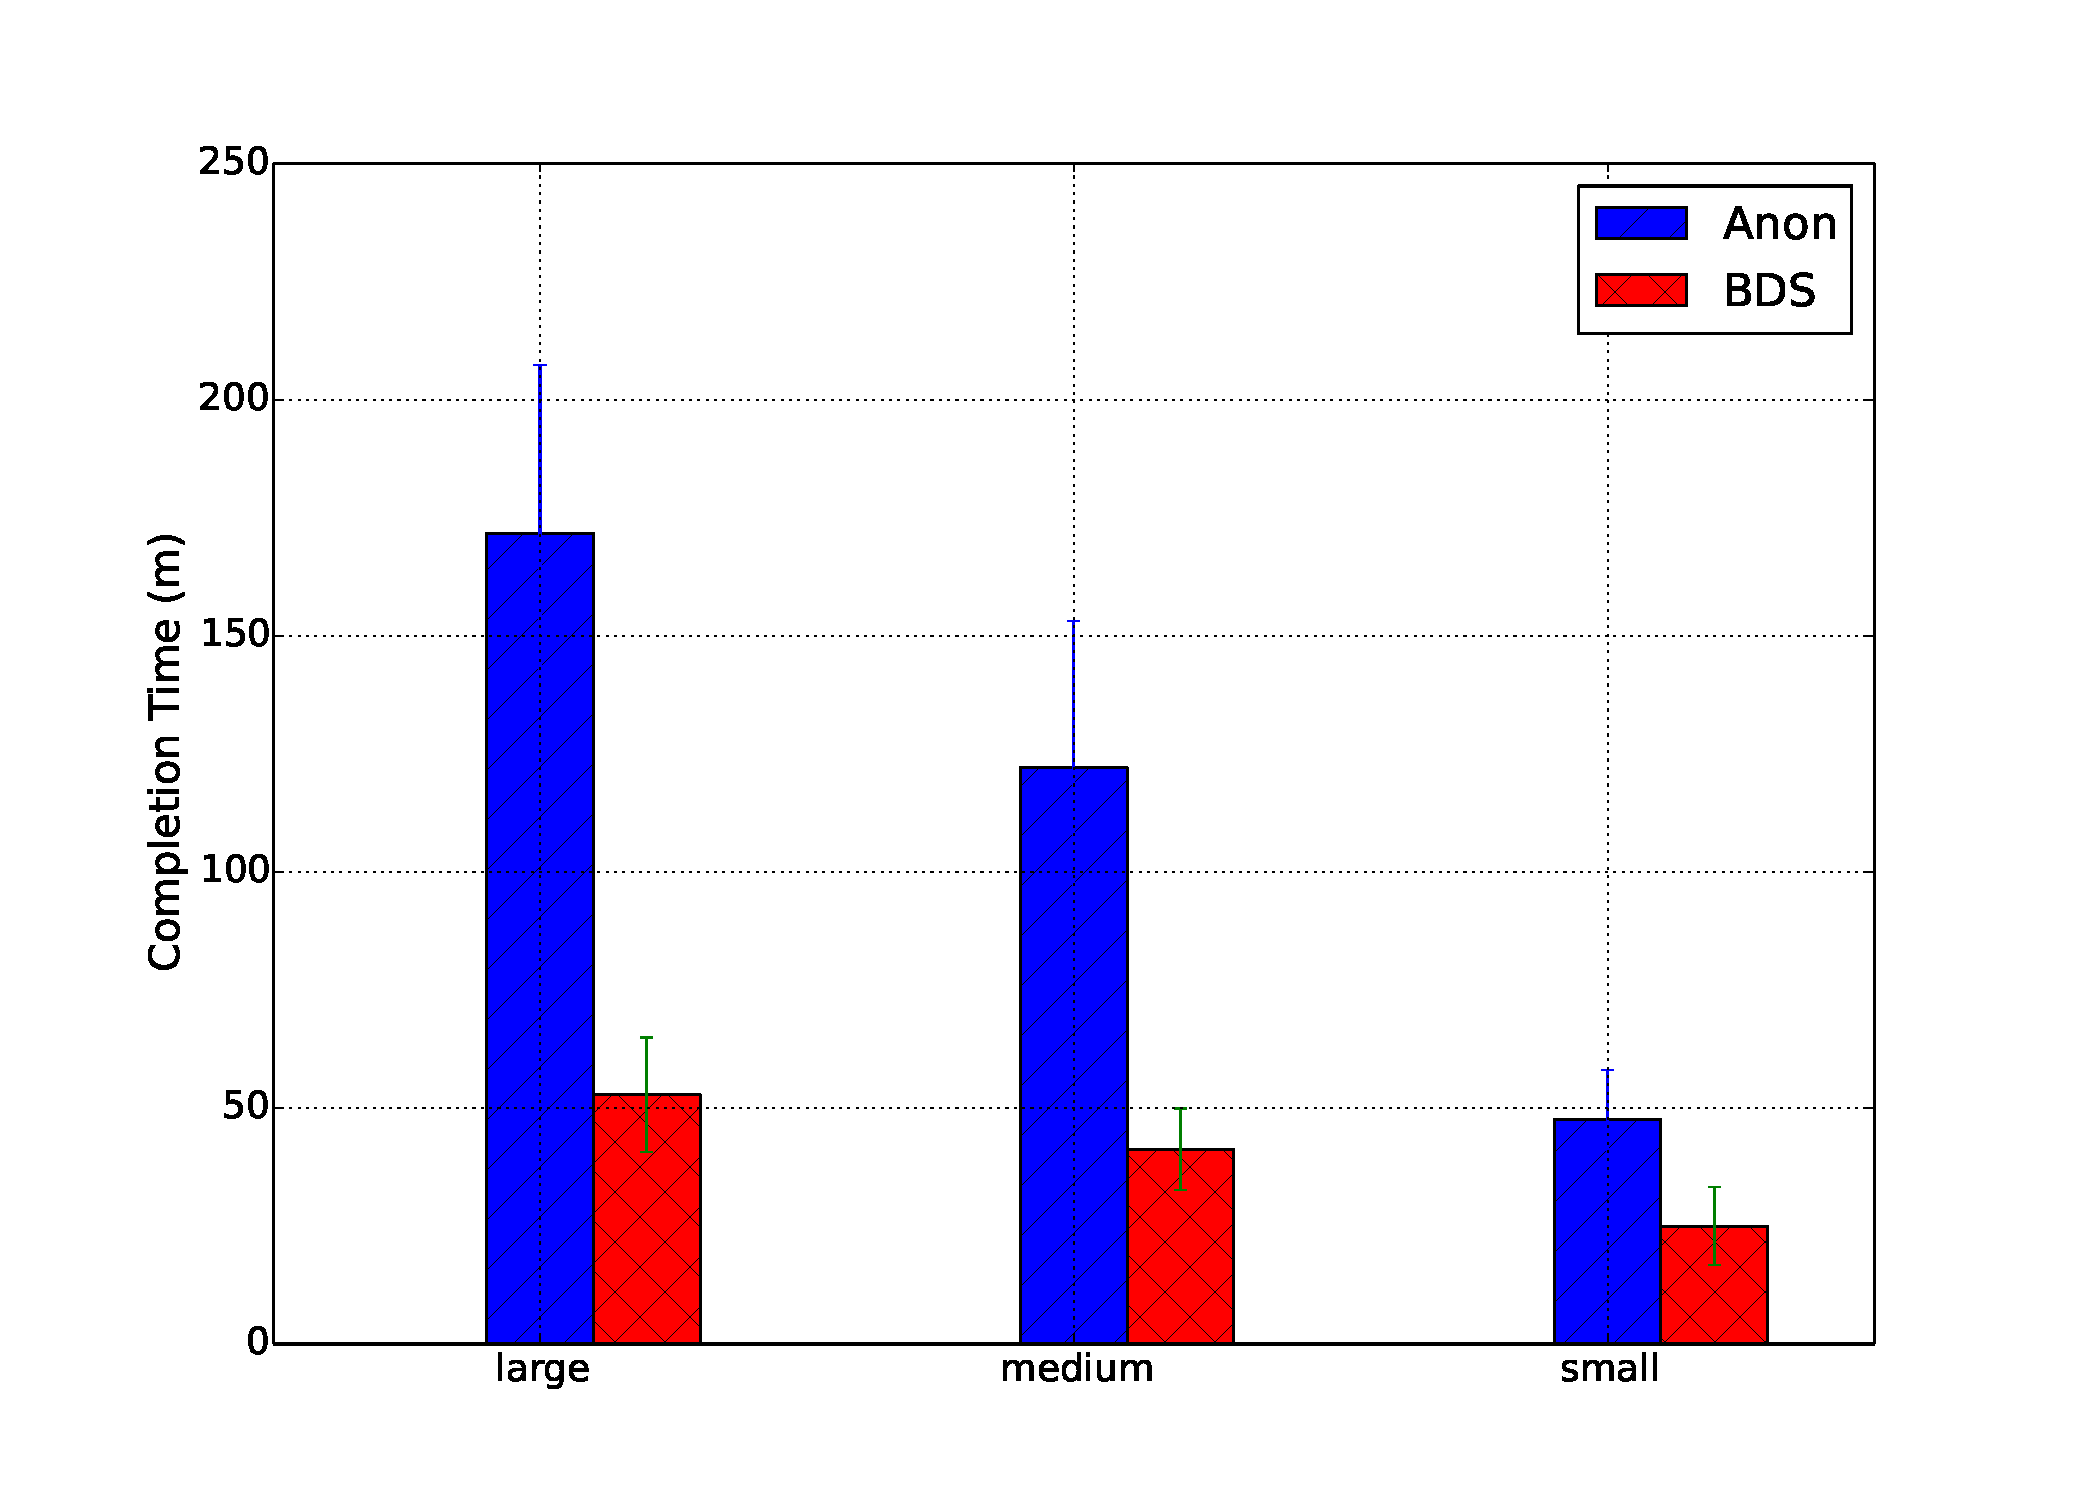
\includegraphics[width=\textwidth]{images/BDS_VS_ANON_v2.eps}
                \caption{Comparison by application types.}
                \label{fig:BDSvsAnon:FCT}
        \end{subfigure}
        \begin{subfigure}[b]{0.3\textwidth}
                \centering
                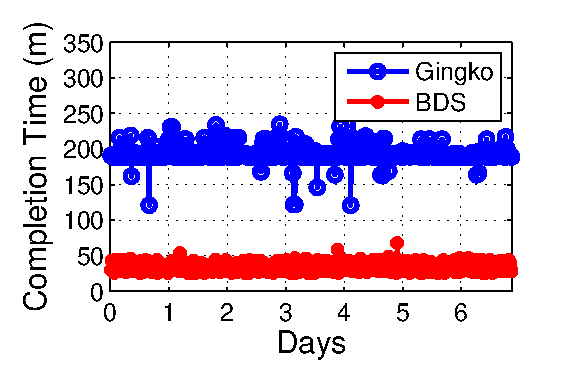
\includegraphics[width=\textwidth]{images/BDSvsAnon_time_v2.eps}
                \caption{Comparison by completion time.}
                \label{fig:BDSvsAnon:time}
        \end{subfigure}
        \tightcaption{[\name vs. \alg (\company's existing solution)] Results from pilot deployments.}
        \label{fig:BDSvsAnon}
\vspace{-0.4cm}
\end{figure*}

%To evaluate \name, we integrated our end-to-end prototype in
%\company, and ran a pilot deployment of \name.
Using a combination of pilot deployment in \company's DCs,
trace-driven simulation, and microbenchmarking, we show that:
\begin{packedenumerate}
\item \name completes inter-DC multicast 3-5$\times$ faster than
\company's existing solutions, as well as other baselines used in
industry (\Section\ref{subsec:evaluation:centralized}).

\NEW{ DELETE:
\item \name significantly reduces the incidents of interferences
between bulk-data multicast traffic and latency-sensitive traffic
(\Section\ref{subsec:evaluation:separation}).
}

\item \name can scale to the traffic demand of a large online
service provider, tolerate various failure scenarios, and achieves
close to optimal flow completion time
(\Section\ref{subsec:evaluation:benchmarks}).


\NEW{ADD: 
\item \newname can: 1. further complete inter-DC multicast XXX$\times$ faster than \name, 2. predict the bandwidth utilization of online traffic with XXX\% accuracy, 3. increase bandwidth utilization when online traffic is in valley, 4. reduces the incidents of interferences caused on bulk-data multicast traffic when online traffic bursts, 5. achieve near real-time scheduling with quite low computation overhead 
(\Section\ref{subsec:evaluation:improvements}).
}
\end{packedenumerate}

\subsection{Performance improvement over existing solutions}
\label{subsec:evaluation:centralized}

\subsubsection{Methodology}

\mypara{Baselines}
We compare \name with three existing solutions: \alg (\company's
existing decentralized inter-DC multi-cast strategy),
Bullet~\cite{kostic2003bullet}, and Akamai's overlay
network~\cite{Andreev2013Designing} (a centralized strategy for
multicasting live videos).


\mypara{Pilot deployment}
We choose several services with different data sizes, and run
A/B testing in which we run \name instead of \company's default
solution \alg for the same hours in several randomly chosen days.

\mypara{Trace-driven simulation}
Complementary to the pilot deployment on real traffic, we also use
trace-driven simulation to evaluate \name on a larger scale.
We simulate the other two overlay multicast techniques using the
same topology, number of servers, and link capacities as \name, and
replay inter-DC multicast data requests in the same chronological
order as in the pilot deployment.

\subsubsection{\name vs. \alg}
\label{subsubsec:name-vs-alg}

We begin by evaluating \name and \alg on one service that needs to
distribute 70~TB data from one source DC to ten destination DCs.
Figure~\ref{fig:BDSvsAnon:overall} shows the cumulative distribution
function (CDF) of the completion time on each destination server. We can
see that the median completion time of \name is 35 minutes,
$5\times$ faster than \alg, where most DCs takes 190 minutes to
get the data.

To generalize the finding, we pick three applications whose data
volumes are large, medium and small, and compare \name's and \alg's
mean (and standard deviation) of completion time for each application
in Figure~\ref{fig:BDSvsAnon:FCT}.
We see that \name consistently outperforms \alg, and has less
performance variance. We also see that \name has greater improvement
in applications with larger data sizes. Finally,
Figure~\ref{fig:BDSvsAnon:time} shows the timeseries of the mean
completion time of \name and \alg in one randomly chosen application,
and we see that \name consistently outperforms \alg by 4$\times$.

\subsubsection{\name vs. other overlay multicast techniques}

Table~\ref{table:versusAkamai} compares \name with two other
baselines, Bullet and Akamai's overlay network, using trace-driven
simulation. We show the results in three setups. In the baseline evaluations,
we send 10TB data from one DC to 11 DCs, each has 100 servers, and
the upload and download link capacities are set to be 20MBs. In the
large-scale evaluations, we send 100TB data between the same DCs, each with
1000 servers. In the rate-limited evaluations, the setup is the same as that in the baseline experiments
except the server upload and download rate limit set to be 5MBs.
We see that \name achieves 3$\times$ shorter completion time than
Bullet and Akamai in the baseline setup, and over 4$\times$ shorter
completion time in the large-scale and small bandwidth setups, which
corroborates the findings in \Section\ref{subsubsec:name-vs-alg} that
\name has greater improvement when data sizes are large.

\begin{table}[t]
\begin{center}
\resizebox{3in}{!}{
%\begin{tabular}{p{2cm}<{\centering}|p{2cm}<{\centering}}
\begin{tabular}{| c | c| c| c|}
\hline
 \rowcolor[gray]{0.9}
\textbf{Solution} & \textbf{Baseline} & \textbf{Large Scale} & \textbf{Rate Limit} \\
\hline \hline
Bullet & $28m$ & $82m$ & $171m$\\
\hline
Akamai & $25m$ & $87m$ & $138m$\\
\hline
\name & $9.41m$ & $20.33m$ & $38.25m$\\
\hline
\end{tabular}
}
\end{center}
\tightcaption{[\name vs. Bullet \cite{kostic2003bullet}, Akamai \cite{Andreev2013Designing}] Completion time of the three solutions in  trace-driven simulation.}
%\caption{Average completion time of Bullet \cite{kostic2003bullet}, Akamai \cite{Andreev2013Designing} and \name.}
\label{table:versusAkamai}
\vspace{-0.4cm}
\end{table}

\subsection{Benefits of coordinated bandwidth allocation}
\label{subsec:evaluation:separation}
\begin{figure}[t]
  \centering
  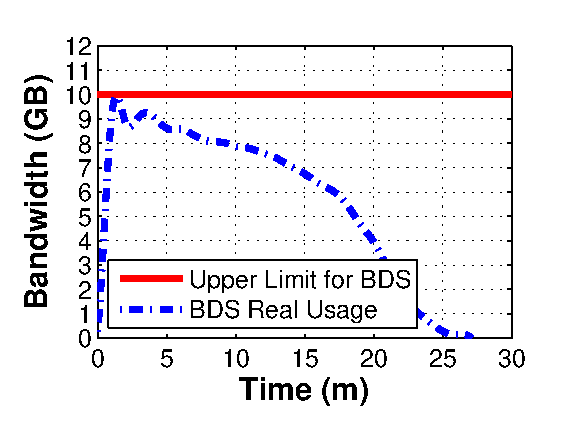
\includegraphics[width=45mm]{images/Quota_v2.eps}%DrawLink.m
  \tightcaption{\color{red}{DELETE: The effectiveness of bandwidth separation.}}
  \label{fig:quota}
\vspace{-0.4cm}
\end{figure}

To reduce the incidences of negative interference between bulk-data
multicast traffic and latency-sensitive traffic, \company sets a
bandwidth limit of bulk data transfers on each link by the difference
between the link capacity and the historical peak bandwidth of
latency-sensitive traffic. Naturally, we can minimize the conflicts,
if \name can keep the bulk-data multicast traffic within the bandwidth
limit. To test \name's effectiveness at maintaining differentiation between
bulk-data multicast traffic and latency-sensitive traffic, we set an
10GB/s bandwidth limit to bulk data transfers.
Figure~\ref{fig:quota} shows the actual bandwidth usage of \name on
one inter-DC link. We can see that in \name the actual bandwidth used
by bulk data is always below 10~GB/s.

%\begin{table}[t]
%\begin{center}
%\resizebox{3in}{!}{%
%%\begin{tabular}{p{2cm}<{\centering}|p{2cm}<{\centering}}
%\begin{tabular}{| c | c | c | c | c |}
%\hline
% \rowcolor[gray]{0.9}
%\textbf{System} & \textbf{Source DC egress link} & \textbf{$l_1$} & \textbf{$l_2$} & \textbf{$l_3$}\\
%\hline \hline
%\alg & 69.82\% & 53.09\% & 57.98\% & 63.01\% \\
%\hline
%\name & 70.55\% & 62.46\% & 63.23\% & 64.24\% \\
%\hline
%\end{tabular}
%}
%\end{center}
%\tightcaption{Average link utilizations of the source DC egress link and 3 inter-DC links ($l_1$, $l_2$, $l_3$) under \alg and \name.}
%\label{table:usage}
%\vspace{-0.4cm}
%\end{table}

\begin{figure*}[t]
        \centering
        \begin{subfigure}[b]{0.3\textwidth}
                \centering
                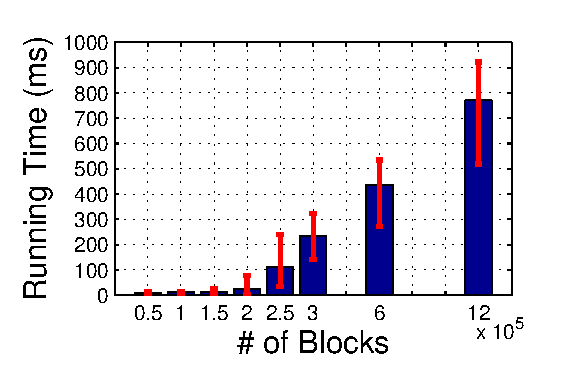
\includegraphics[width=50mm]{images/CPUvsBlk_v3.eps}% cpu.m replaced by running_time.m
                \caption{The controller running time.}
                \label{fig:scale:cpu}
        \end{subfigure}
        \begin{subfigure}[b]{0.3\textwidth}
                \centering
                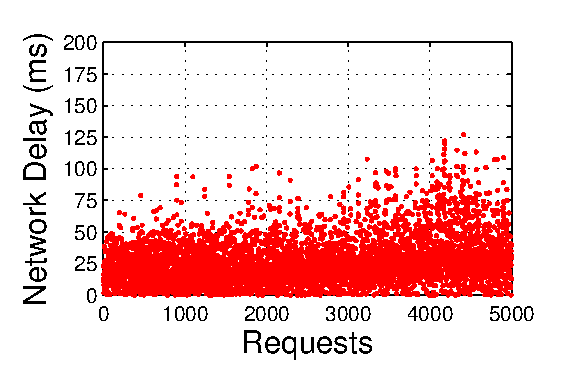
\includegraphics[width=50mm]{images/NetworkDelay.eps}%CDFofNetworkDelay -> Communication.m
                \caption{The inter-DC network delay.}
                \label{fig:scale:network}
        \end{subfigure}
        \begin{subfigure}[b]{0.3\textwidth}
                \centering
                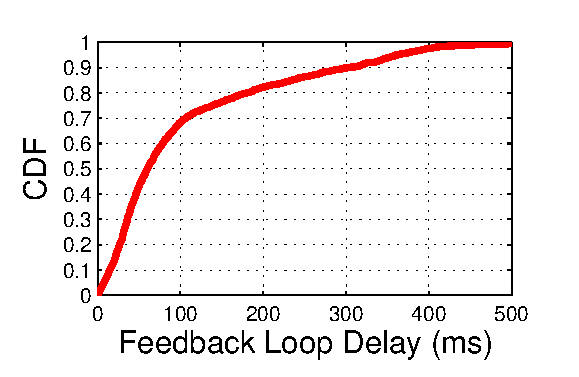
\includegraphics[width=50mm]{images/CDFofFeedbackLoopDelay.eps}
                \caption{Feedback loop delay.}
                \label{fig:scale:feedback}
        \end{subfigure}
        \tightcaption{[System scalability] Measurements on (a) controller running time, (b) network delay, (c) Feedback loop delay.}
        \label{fig:scale}
\vspace{-0.4cm}
\end{figure*}

\begin{figure*}[t]
        \centering
        \begin{subfigure}[b]{0.3\textwidth}
                \centering
                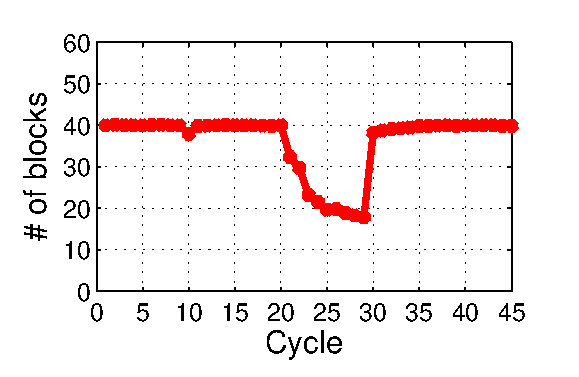
\includegraphics[width=50mm]{images/failure_v2.eps}%fail.m
                \caption{Average number of downloaded blocks per cycle under failures.}
                \label{fig:analysis:failure}
        \end{subfigure}
        \begin{subfigure}[b]{0.3\textwidth}
                \centering
                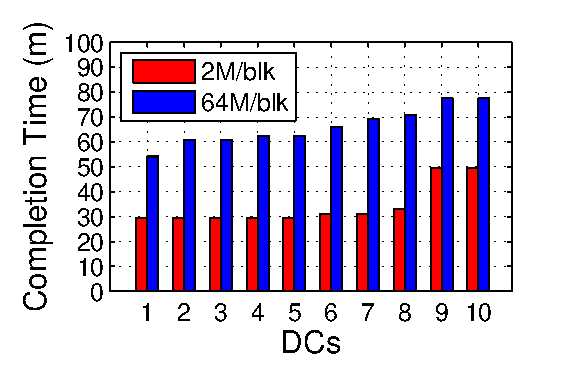
\includegraphics[width=50mm]{images/blkSize_v2.eps} %plotTCT_IDC.m
                \caption{Completion time under different block sizes.}
                \label{fig:analysis:blksize}
        \end{subfigure}
        \begin{subfigure}[b]{0.3\textwidth}
                \centering
                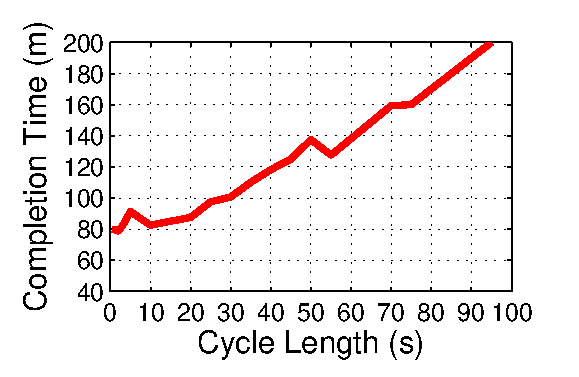
\includegraphics[width=50mm]{images/cycleDiff.eps}%cycleDiff.m
                \caption{Completion time under different cycle lengths.}
                \label{fig:analysis:cycleDiff}
        \end{subfigure}
%        \begin{subfigure}[b]{0.3\textwidth}
%                \centering
%                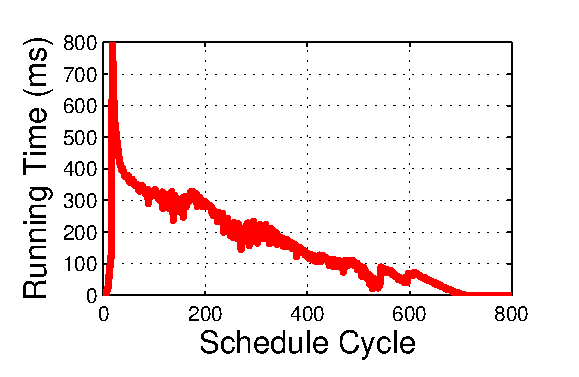
\includegraphics[width=50mm]{images/cycle.eps} %calculation_origin
%                \caption{Reduction on algorithm running time due to approximation.}
%                \label{fig:analysis:time}
%        \end{subfigure}
%        \begin{subfigure}[b]{0.3\textwidth}
%                \centering
%                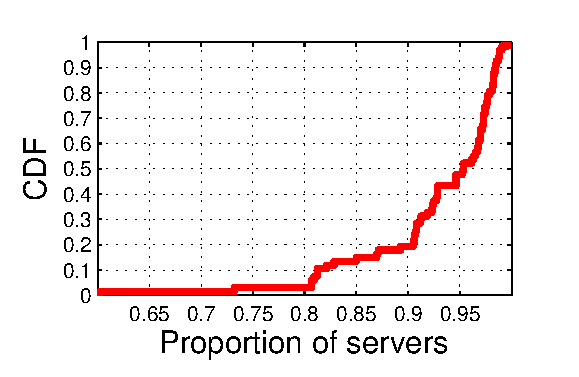
\includegraphics[width=50mm]{images/overlay.eps}
%                \caption{The proportion of blocks downloaded from the original source.}
%                \label{fig:analysis:overlay}
%        \end{subfigure}
        \tightcaption{\name's (a) fault tolerance, (b) sensitivity to different block sizes, and (c) different cycle lengths.}
        \label{fig:analysis}
\vspace{-0.4cm}
\end{figure*}


%\jc{i'm totally lost... what's the point of this para?}
%As \name implements strict bandwidth separation between latency-sensitive traffic and bulk data transfers while still showing shorter completion time, does it occupy too much bandwidth on inter-DC links? To answer this question, we record the average utilizations of the egress link of the source DC and 3 randomly selected inter-DC links, denoted as $l_1,l_2$ and $l_3$. The result in Table \ref{table:usage} shows that link utilizations do not change much with \name. This is because \name spreads data transfers over bottleneck-disjoint paths, so it avoids transferring the same data on the same link.

%\begin{itemize}
%\item Draw a graph (what graph can you get on this?) to show with bandwidth separation, \name can reduce the incidents of delay on latency-sensitive traffic caused by bulk data transfers.%DrawLink.m
%\item Draw a graph (what graph can you get on this?) to show the link utilization does not change much with \name or with \company.%DrawUsage.m
%\end{itemize}

\subsection{Micro-benchmarks}
\label{subsec:evaluation:benchmarks}

Next, we use micro-benchmarking to evaluate \name along three metrics:
(1) scalability of the centralized control;
(2) fault tolerance; and
(3) optimality of \name parameters.

\subsubsection{Scalability}
\label{subsec:evaluation:benchmarks:scalability}

\mypara{Controller running time}
As the controller needs to decide the scheduling and routing of each
data block, the running time of the control logic naturally scales
with the number of blocks. Figure~\ref{fig:scale:cpu} shows the
running time as a function of the total number of blocks. We can see
that the centralized \name controller can update the scheduling and
routing decision within 800ms with $10^6$ blocks. To put this number
into perspective, in \company's DCs, the maximum number of simultaneous
outstanding data blocks is around $3\times 10^5$, for which \name can
finish updating the decisions within 300ms.

\mypara{Network delay} \name works in inter-DC networks, so the network delay among DCs is a key factor in the algorithm updating process. We recorded the network delay of 5000 requests and present the CDF in Figure \ref{fig:scale:network}. We can see that 90\% of the network delays are below $50ms$ and the average value is about $25ms$, which is less than 1\% of the decision updating cycle (3 seconds).

\mypara{Feedback loop delay} For centralized algorithms, a small feedback loop delay is essential for algorithmic scalability. In \name, this feedback loop consists of several procedures: status updating from agents to the controller, running of the centralized algorithm, and decision updating from the controller back to agents. We measure the delay of the whole process, as shown in the CDF of Figure \ref{fig:scale:feedback}, and find that in most cases (over 80\%), the feedback loop delay is lower than $200ms$. So we claim that \name demonstrates a short enough latency and is able to scale to even larger systems.

\begin{figure*}[t]
        \centering
        \begin{subfigure}[b]{0.3\textwidth}
                \centering
                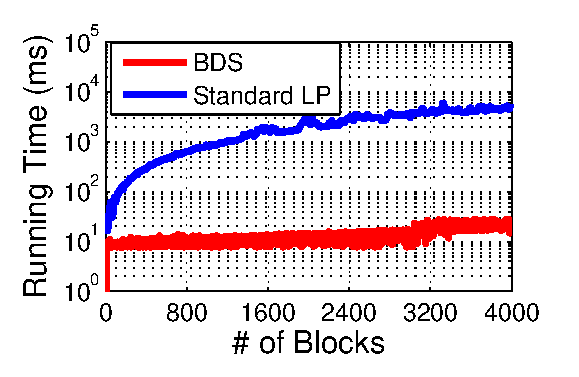
\includegraphics[width=50mm]{images/BDSvsLP_v2.eps} % BDSvsLP.m
                \caption{The reduction on algorithm running time of \name over standard LP.}
                \label{fig:further:BDSvsLP}
        \end{subfigure}
        \begin{subfigure}[b]{0.3\textwidth}
                \centering
                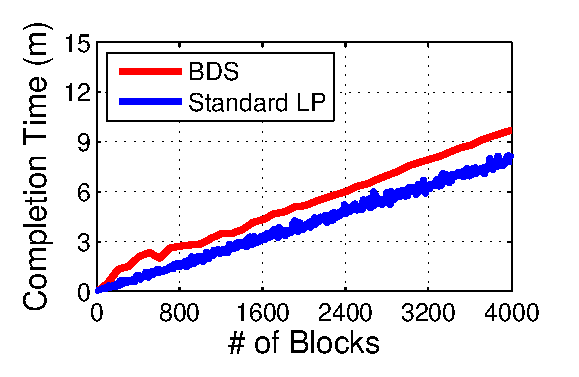
\includegraphics[width=50mm]{images/BDSvsLP_CT.eps}%BDSvsLP_CT -> Communication.m
                \caption{The near-optimality of \name to standard LP in small scale.}
                \label{fig:further:BDSvsLP_CT}
        \end{subfigure}
        \begin{subfigure}[b]{0.3\textwidth}
                \centering
                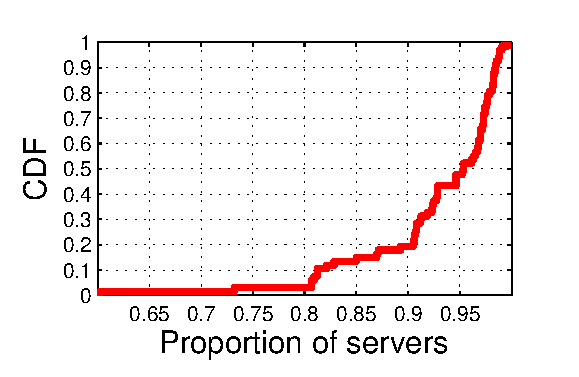
\includegraphics[width=50mm]{images/overlay.eps}
                \caption{The proportion of blocks downloaded from the original source.}
                \label{fig:further:overlay}
        \end{subfigure}
        \tightcaption{[In-depth analysis] on (a) reduction on algorithm running time, (b) near-optimality, and (c) effects of overlay transmission.}
        \label{fig:further}
\vspace{-0.4cm}
\end{figure*}

%\tightsubsubsection{Algorithm adaptability.}\label{subsubsec:evaluation:adaptability}
\subsubsection{Fault tolerance}

%\mypara{Fault tolerance}
Here we examine the impact of the following failure scenario on the number of downloaded blocks per cycle. During cycles 0 to 9, \name works as usual, and one agent fails in the 10th cycle. The controller fails in the 20th cycle and recovers in the 30th cycle. Figure \ref{fig:analysis:failure} shows the average number of downloaded blocks per cycle. We find that the slight impact of agent failure only lasts for one cycle, and the system recovers in the 11th cycle. When the controller is unavailable, \name falls back to a default decentralized overlay protocol, resulting in graceful performance degradation. With the recovery of the controller, the performance recovers in the 30th cycle.

\subsubsection{Choosing the values of key parameters}\label{subsec:evaluation:benchmarks:parameters}

\mypara{Block size} In \name, the bulk data file is split into blocks and can be transferred on bottleneck-disjoint paths. But this introduces a tradeoff between scheduling efficiency and calculation overhead. We therefore conduct two series of experiments using different block sizes (2MB and 64MB). Figure \ref{fig:analysis:blksize} shows that the completion time in the 2MB/block scenario is 1.5 to 2 times shorter than that in the 64MB/block scenario.
%This is because a smaller block sizes result in closer-to-optimal performance (see Appendix for the proof).
However, this optimization introduces a longer controller running time, as shown in Figure \ref{fig:scale:cpu}. We pick block size by balancing two considerations: (1) constraints on the completion time, and (2) the controller's operational overhead.

\mypara{Update cycle lengths} Since any change in network environment may potentially alter the optimal overlay routing decisions, \name reacts to the changing network conditions by adjusting the routing scheme periodically. To test the adjustment frequency, we set different cycle lengths from $0.5s$ to $95s$ for the same bulk data transfer, and Figure \ref{fig:analysis:cycleDiff} shows the completion time. Smaller cycle lengths result in shorter completion time, but the benefit diminishes when the cycle length is less than $3s$. This is because updating too frequently introduces greater overhead on: (1) the information collection from agents to the controller, (2) the execution of the centralized algorithm, and (3) the re-establishment of new TCP connections. Thus, considering adjustment granularity and the corresponding overhead, we finally choose $3s$ as the default cycle length.


\tightsubsubsection{In-depth analysis.}\label{subsubsec:evaluation:depth}

\mypara{Optimization over algorithm running time} \name decouples scheduling and routing, which can significantly reduce the computational complexity. To clearly show the optimization, we measure the algorithm running time under \name and the standard LP solution. For the standard LP experiments, we use the \textit{linprog} library on MATLAB \cite{mathworks}, set the upper bound of the iteration number ($10^6$) if the algorithm does not converge, and record the CPU time as a function of the block number. Figure \ref{fig:further:BDSvsLP} shows that the running time of \name keeps below $25ms$ while that of standard LP grows quickly to $4s$ with only 4000 blocks. %This result illustrates \name's optimization over algorithm running time.
\name is much faster than an off-the-shelf LP solver.

\mypara{Near-optimality of \name} To measure the near-optimality, we evaluate the data transfer completion time under the standard LP and \name: 2 DCs, 4 servers, 20MBs for server upload/download rate.
%1 to 4000 blocks (we cannot conduct large-scale experiments due to the explosive growth of the LP calculation time).
We vary the number of blocks from 1 to 4000, over which the LP solver cannot finish in a reasonable time. Figure \ref{fig:further:BDSvsLP_CT} shows the near-optimality of \name.%that the difference of completion time between \name and the optimal standard LP is about 15\%.


\mypara{Benefit of disjoint overlay paths} \Section\ref{subsec:motivation:case-for} reveals the benefits of disjoint paths on application-level overlay networks. To explore the potential benefit, we record the ratio of the number of blocks downloaded from the original source to the total number of blocks, and the CDF is shown in Figure \ref{fig:further:overlay}. For about 90\% of servers, the proportion is less than 20\%, which means that more than 80\% blocks are downloaded from other DCs on the disjoint paths, demonstrating the great potential of a multicast overlay network.

%\mypara{Breakdown of feedback loop delay} \name also applies the approximation of separating data scheduling from overlay routing, which can also reduce algorithm running time. We show the measurements on algorithm running time in Figure \ref{fig:analysis:time}. At the very beginning, the running time is nearly $800ms$, but drops to $300ms$ and even less quickly. This is because the separated scheduling stage selects only a subset of blocks, making the number of blocks decrease significantly and simplifying the routing decision making process.


%\begin{figure*}[t]
%        \centering
%        \begin{subfigure}[b]{0.3\textwidth}
%                \centering
%                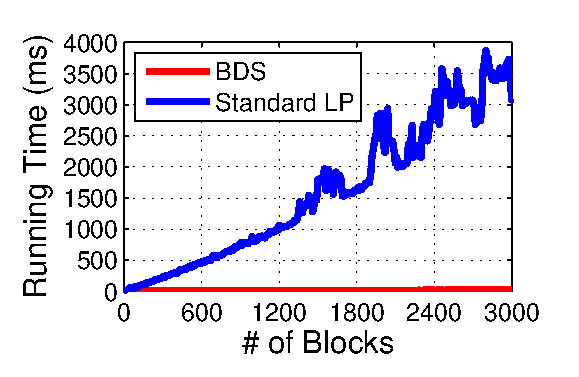
\includegraphics[width=50mm]{images/BDSvsLP.eps} % BDSvsLP.m
%                \caption{Algorithm running time of \name and standard LP.}
%                \label{fig:further:BDSvsLP}
%        \end{subfigure}
%        \begin{subfigure}[b]{0.3\textwidth}
%                \centering
%                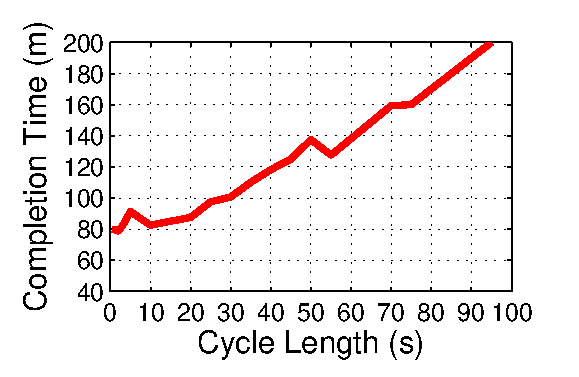
\includegraphics[width=50mm]{images/cycleDiff.eps}%cycleDiff.m
%                \caption{Completion time under different cycle lengths.}
%                \label{fig:further:cycleDiff}
%        \end{subfigure}
%        \begin{subfigure}[b]{0.3\textwidth}
%                \centering
%                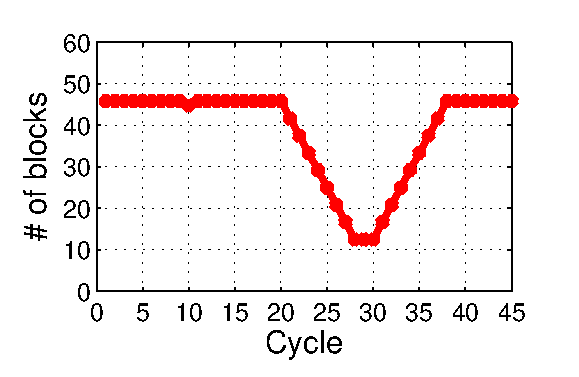
\includegraphics[width=50mm]{images/failure.eps}%fail.m
%                \caption{Average number of downloaded blocks per cycle under failures.}
%                \label{fig:further:failure}
%        \end{subfigure}
%        \caption{Further analysis on (1) running time, (2) cycle length, and (3) fault tolerance.}
%        \label{fig:further}
%\vspace{-0.4cm}
%\end{figure*}
\NEW{
\subsection{\newname's dynamic bandwidth separation}
\label{subsec:evaluation:improvements}
Evaluations between \newname and \name.

1. further complete inter-DC multicast XXX$\times$ faster than \name, 

2. predict the bandwidth utilization of online traffic with XXX\% accuracy, 

3. increase bandwidth utilization when online traffic is in valley, 

4. reduces the incidents of interferences caused on bulk-data multicast traffic when online traffic bursts, 

5. achieve near real-time scheduling with quite low computation overhead

\subsubsection{Completion time}
\label{subsec:evaluation:completaiontime}
\begin{figure}[t]
  \centering
  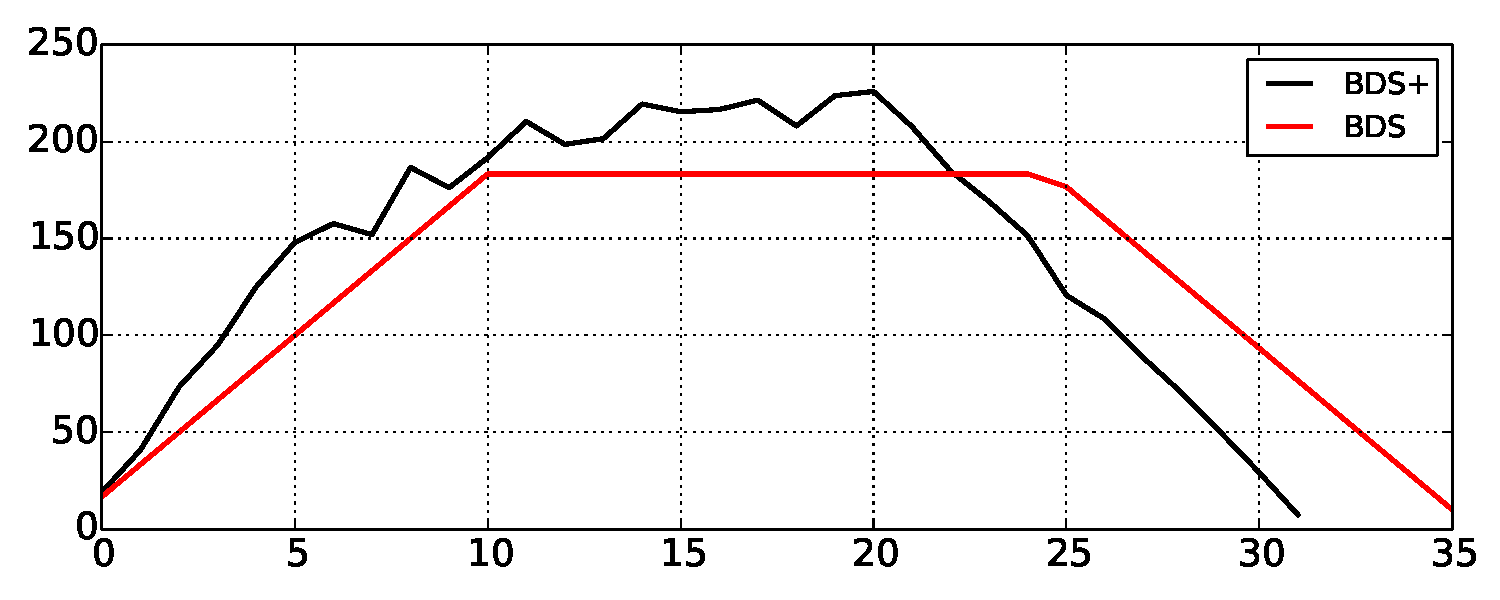
\includegraphics[width=80mm]{images/bds+/average_downloaded_blk_per_cycle.pdf}
  \tightcaption{Average downloaded block number in each cycle.}
  \label{fig:quota}
\vspace{-0.4cm}
\end{figure}
\subsubsection{Accuracy of the prediction algorithm}
\label{subsec:evaluation:algaccuracy}
\begin{figure}[t]
  \centering
  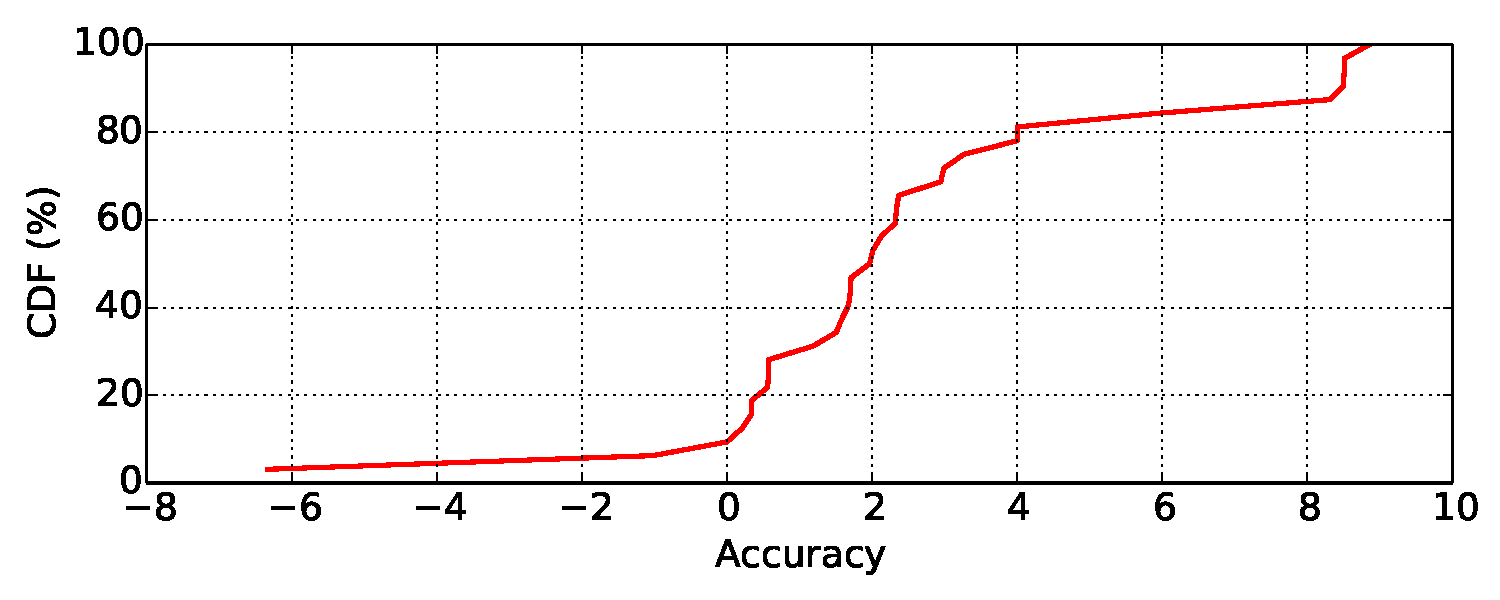
\includegraphics[width=80mm]{images/bds+/alg_accuracy.pdf}
  \tightcaption{The accuracy distribution of prediction algorithm.}
  \label{fig:quota}
\vspace{-0.4cm}
\end{figure}
\subsubsection{Bandwidth utilization}

Show that we can use much more bandwidth when online traffic is in valley.

Can show the number of additional blocks that are transferred in each big scheduling cycle. 

\subsubsection{Reduces the incidents}

Show that we can reduce bandwidth that is allocated to bulk-data transfer when online traffic bursts.

Can show the number of blocks that are cancelled in each big scheduling cycle. 

\subsubsection{Computation overhead}

Show the rate of links that are affected by the predicted algorithm (i.e., on which links the bandwidth can be increased/reduced).

Show the computation latency of the bandwidth adjustment algorithm.

}
\label{subsec:evaluation:computationoverhead}
\begin{figure}[t]
  \centering
  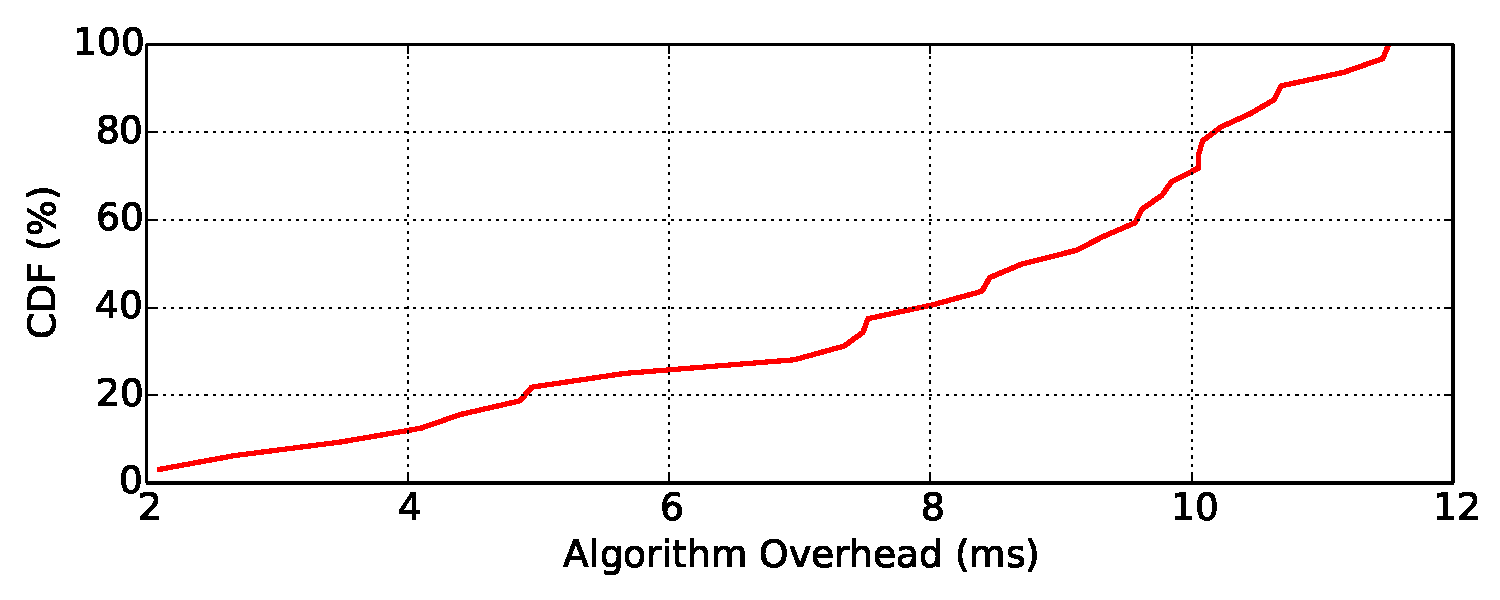
\includegraphics[width=80mm]{images/bds+/alg_overhead.pdf}
  \tightcaption{Computation overhead of prediction algorithm}
  \label{fig:quota}
\vspace{-0.4cm}
\end{figure}
In summary, both the prototype pilot deployment and the trace-driven simulations of \name show 3-5$\times$ speedup over existing solutions, with good scalability and reliability, and near-optimal scheduling results \NEW{ while \newname can work harmoniously with online traffic and further completes inter-DC multicast XXX times faster}.


%\begin{itemize}
%\item Scalability of centralized control:
%\begin{itemize}
%\item Y: Bandwidth consumption, vs. X: \# of objects
%\item Y: Controller CPU usage, vs. X: \# of objects
%\item Y: Update delay vs. X: \# of objects
%\item Bar-chart to decompose update delay into collecting updates, running algorithm, and updating local agents
%\end{itemize}
%
%\item In-depth analysis:
%\begin{itemize}
%\item A graph to show the tradeoff caused by different update cycles (why 3 seconds is a good tradeoff?)
%\item Reduction on algorithm running time due to the approximation algorithm.
%\item Maybe another graph from the current 6.3?
%\end{itemize}
%
%\item Fault tolerance:
%\begin{itemize}
%\item Y: flow completion time, vs. X: time. Create a toy topology to send objects. The experiment begins with no failure. At time t1, one server is not available, and the graph should show Y only has performance degradation for less than 3 seconds; At time t2, the controller is not available, and the local agent should automatically revert to decentralized local control.
%\end{itemize}
%
%\end{itemize}






\section{Evaluation}
\label{sec:evaluation}
\begin{figure*}[t]
        \centering
        \begin{subfigure}[b]{0.3\textwidth}
                \centering
                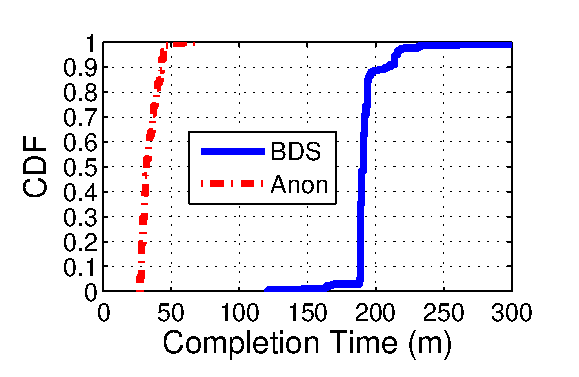
\includegraphics[width=\textwidth]{images/BDSvsAnon_overall.eps}
                \caption{Distribution of completion time.}
                \label{fig:BDSvsAnon:overall}
        \end{subfigure}
        \begin{subfigure}[b]{0.3\textwidth}%@X:\6 PieBridge\simulation\beijing\3 Applications\plot
                \centering
                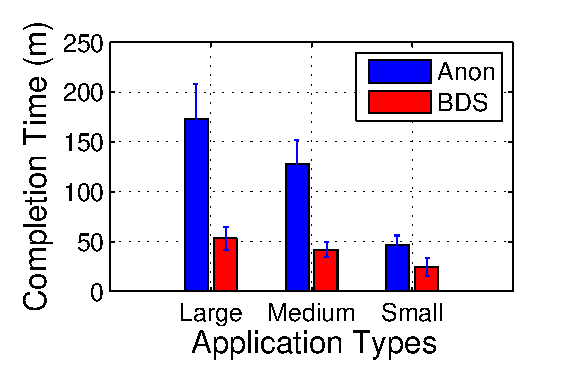
\includegraphics[width=\textwidth]{images/BDS_VS_ANON_v3.eps}
                \caption{Comparison by application types.}
                \label{fig:BDSvsAnon:FCT}
        \end{subfigure}
        \begin{subfigure}[b]{0.3\textwidth}
                \centering
                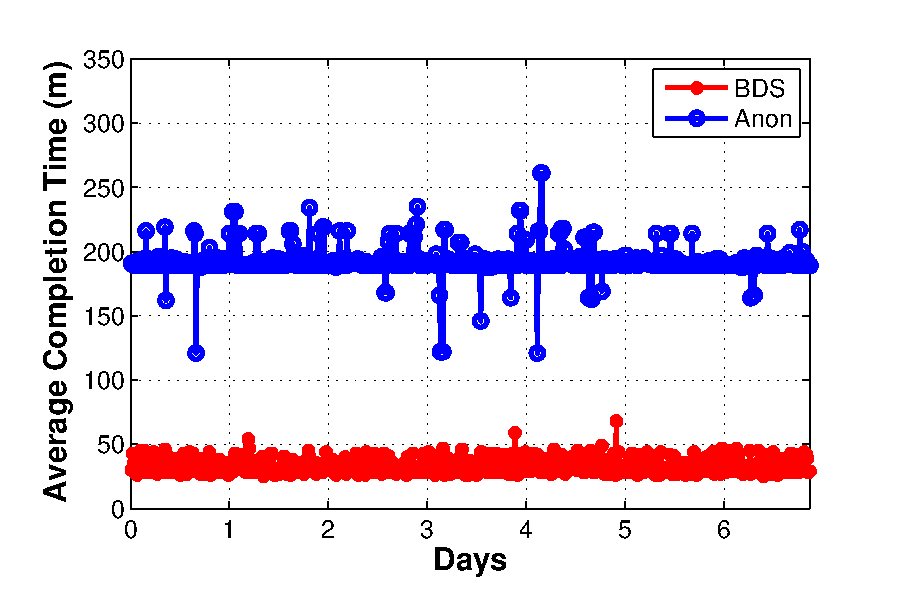
\includegraphics[width=\textwidth]{images/BDSvsAnon_time.eps}
                \caption{Comparison by completion time.}
                \label{fig:BDSvsAnon:time}
        \end{subfigure}
        \tightcaption{[\name vs. \company] Results from pilot deployments.}
        \label{fig:BDSvsAnon}
\vspace{-0.4cm}
\end{figure*}

To evaluate \name, we integrated our end-to-end prototype in \company, and ran a pilot deployment under the above implementation.
Using a combination of pilot deployment, trace-driven simulation, and microbenchmarking, we show that:
\begin{packedenumerate}
\item \name completes inter-DC multicast 3-5$\times$ faster than \company's existing solution and other baselines used in industry (\Section\ref{subsec:evaluation:centralized}).
\item \name significantly reduces the incidents of interferences between bulk-data multicast traffic and latency-sensitive traffic (\Section\ref{subsec:evaluation:separation}).
\item \name can scale to the traffic demand of a large online service provider, tolerate various failure scenarios, and is close to the theoretically optimal performance (\Section\ref{subsec:evaluation:benchmarks}).
\end{packedenumerate}

%\begin{figure*}[t] %@X:\6 PieBridge\simulation\DrawFig
%        \centering
%        \begin{subfigure}[b]{0.3\textwidth}
%                \centering
%                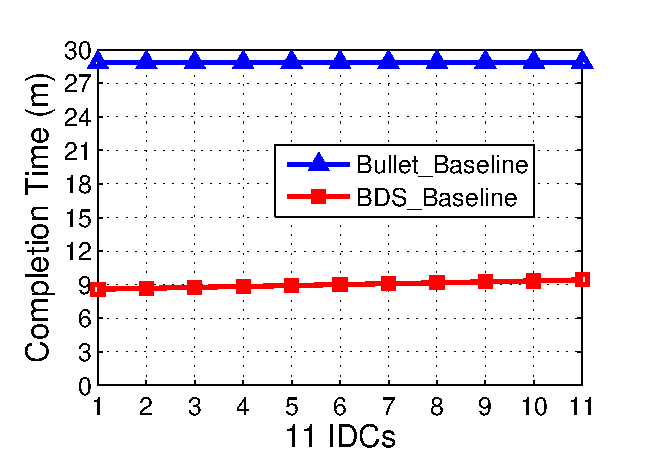
\includegraphics[width=50mm]{images/Test1.eps}
%                \caption{Baseline experiment.}
%                \label{fig:cdn:baseline}
%        \end{subfigure}
%        \begin{subfigure}[b]{0.3\textwidth}
%                \centering
%                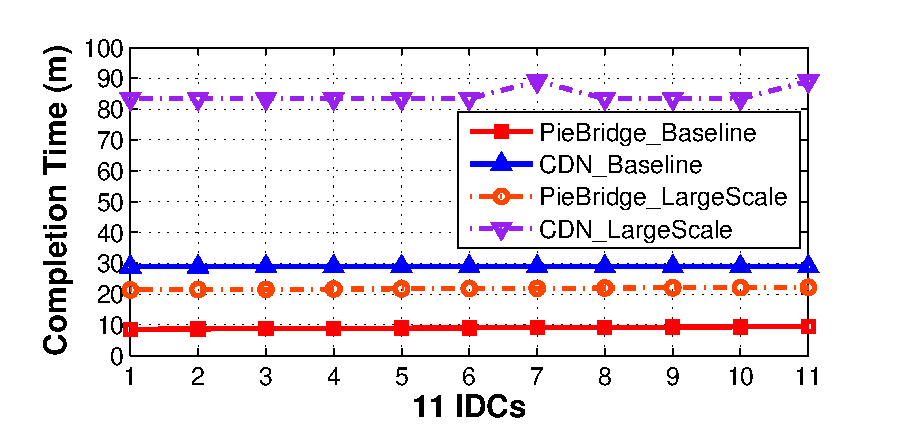
\includegraphics[width=50mm]{images/Test2.eps}
%                \caption{Large scale experiments.}
%                \label{fig:cdn:scale}
%        \end{subfigure}
%        \begin{subfigure}[b]{0.3\textwidth}
%                \centering
%                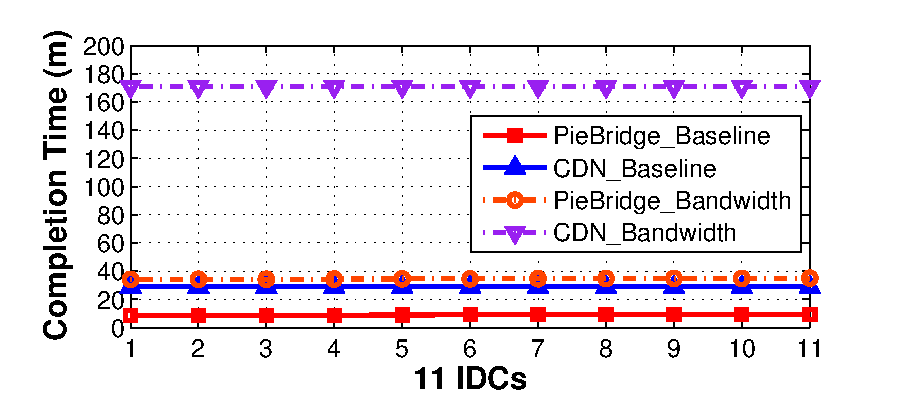
\includegraphics[width=50mm]{images/Test3.eps}
%                \caption{Small bandwidth experiments.}
%                \label{fig:cdn:bw}
%        \end{subfigure}
%        \caption{[\name versus Bullet] Comparisons under different network scenarios.}
%        \label{fig:versusCDN}
%\vspace{-0.4cm}
%\end{figure*}


\subsection{Performance improvement over existing solutions}
\label{subsec:evaluation:centralized}

We compare \name against three existing solutions:
\company's existing solution (a decentralized strategy which has been evolving for 5 years with end-to-end evaluations),
Bullet~\cite{kostic2003bullet} (a centralized strategy), and
Akamai's overlay network~\cite{Andreev2013Designing} for live video streaming
multicast.


\tightsubsubsection{Methodology}
We start with the methodology.

\mypara{Pilot deployment} We choose several services with different data sizes and run randomized A/B testing in which
%In general, such bulk data is transferred using \company's existing solution (that has already run for more than 5 years), while
we randomly choose several days to use \name instead of the current solution. To make sure that the two solutions work in the similar environment, we conduct all the experiments at 02:00 every day in the morning.

\mypara{Trace-driven simulation} Complementary to the pilot deployment on real traffic, we also use trace-driven simulation to evaluate \name on a larger scale.
%than the pilot deployment cannot implement other solutions on \company's real network. Instead,
We simulate the other two overlay multicast techniques by setting topology, DC scale and configuring servers with the same scale as \name's DCs, and replay inter-DC multicast data requests in the same chronological
order as in the pilot deployment (including the number of requests and the number of nodes).


%To evaluate the benefits of centralized control, we conduct two series of experiments: the comparisons with \company's existing solution based on the pilot deployments, and the comparisons with other overlay multicast techniques using trace-driven simulations.

\tightsubsubsection{\name vs. \company's existing solution}

We first choose one service with 70~TB aggregated daily bulk data, which is distributedly stored in the source DC. Each of the other DCs downloads a copy of the data and stores it in the same distributed way.

%First of all, we present the completion time of destination servers under \name and \company in Figure

To intuitively present the overall improvements by \name, we draw the cumulative distribution function (CDF) of the completion time in Figure \ref{fig:BDSvsAnon:overall}, from which we can see that the completion time under \company's existing solution is about 200 minutes while that under \name is less than 40 minutes, which is 5 times shorter.

For detailed illustration, we further pick three applications whose data volumes are large, medium and small, and compare \name's and \company's mean (stddev) completion time for each application in Figure \ref{fig:BDSvsAnon:FCT}.
%draw three pairs of bar charts in Figure \ref{fig:BDSvsAnon:FCT}, each representing \name's and \company's mean (stddev) completion time for one application.
These bars show that the benefit of \name increases along with the bulk data size. For small data volume, \name outperforms \company by 1.6 times, and more than 3 times than \company for large-data transfers.

We also repeat the experiments for 7 days to offer more statistical significance and draw the average completion time of both \name and \company in Figure \ref{fig:BDSvsAnon:time}. \name consistently outperforms \company by 4 times, and has less performance variations.
%is quite stable during these 7 days while \company illustrates some volatilities.
In general, \name achieves about 4.5 times shorter completion time than \company.
%\item \name vs. \company's existing solution (pilot deployment)
%\begin{itemize}
%\item Overall improvement: A CDF with two lines to show the aggregated flow completion time
%\item By applications: Pick three applications whose data volumes are large, medium, and small respectively. Draw a bar chart of three pairs of bars, each representing \name's and \company's mean (stddev) flow completion time for an application.
%\item By time: Timeseris of two lines, each representing \name's and \company's mean (stddev) of flow completion time.
%\end{itemize}

\tightsubsubsection{\name vs. other overlay multicast techniques}

%As we cannot implement other experimental systems in our real online network just as comparisons, we conduct a series of simulations using trace-driven simulations in this section, and compare \name's performance versus Bullet \cite{kostic2003bullet} and a CDN-based solution \cite{Andreev2013Designing} adopted by Akamai.

For \company's infrastructure, there are 1k to 20k servers in each DC, but there is no need for \name to be deployed in all the servers because only some of these servers are used for bunk data transfer. In the trace-driven simulations, we use a topology with 11 DCs (one of which acts as the source DC) and set all the parameters to be the same as for the real network, including data file size, data source and destination, paths, link capacities and server upload/download rates. We use two baselines: Bullet \cite{kostic2003bullet} is a data dissemination system using an overlay mesh, and Akamai's video streaming system \cite{Andreev2013Designing} in overlay multicast networks.

%We conduct three series of experiments and show the results in Figure \ref{fig:versusCDN}: baseline \ref{fig:cdn:baseline}, large scale \ref{fig:cdn:scale} and small bandwidth experiments \ref{fig:cdn:bw}. We find \name achieves 3$\times$ shorter completion time than Bullet in the baseline experiments, and more than 4$\times$ improvement in the large scale experiments and small bandwidth experiments.
We conduct three series of experiments and show the results in Table \ref{table:versusAkamai}: baseline, large-scale and small bandwidth experiments. In the baseline experiments, the size of the bulk data is 10TB, the number of servers per DC is 100, and the upload and download rate limits are set to 20MBs. In the large-scale experiment, the bulk data is 100TB, server number per DC is 1000. In the small bandwidth experiment, server upload and download rate limit are reduced to 5MBs. We find that \name achieves 3 times shorter completion time than Bullet and Akamai in the baseline experiments, and more than 4 times shorter completion time in the large-scale and small bandwidth experiments.

Considering the results in large-scale experiments, we found that the completion time of Bullet (and Akamai) increase to more than 3 times compared that in the baseline experiments - from $28m$ (and $25m$)to about $82m$ (and $87m$), while \name only increases to about 2 times - from $9.41m$ to $20.33m$. This proves \name's good scalability. Similarly, in the small bandwidth experiments (which is very common when delay-sensitive traffic bursts), the completion time of Bullet and Akamai increases to $171m$ and $138m$, respectively, while that of \name is just $38.25m$. This result illustrates the high efficiency of \name under strict bandwidth limitations.
%In the large scale experiments, the completion time of Bullet increases to about 3 times than that in the baseline experiment, and that of Akamai multicast solution is about 3.5 times. But \name., \name increase to while that of respectively.

\begin{table}[t]
\begin{center}
\resizebox{3in}{!}{
%\begin{tabular}{p{2cm}<{\centering}|p{2cm}<{\centering}}
\begin{tabular}{| c | c| c| c|}
\hline
 \rowcolor[gray]{0.9}
\textbf{Solution} & \textbf{Baseline} & \textbf{Large Scale} & \textbf{Rate Limit} \\
\hline \hline
Bullet & $28m$ & $82m$ & $171m$\\
\hline
Akamai & $25m$ & $87m$ & $138m$\\
\hline
\name & $9.41m$ & $20.33m$ & $38.25m$\\
\hline
\end{tabular}
}
\end{center}
\tightcaption{[\name vs. Bullet \cite{kostic2003bullet}, Akamai \cite{Andreev2013Designing}] Completion time of the three solutions in  trace-driven simulation.}
%\caption{Average completion time of Bullet \cite{kostic2003bullet}, Akamai \cite{Andreev2013Designing} and \name.}
\label{table:versusAkamai}
\vspace{-0.4cm}
\end{table}

%\begin{itemize}
%\item \name vs. other overlay multicast techniques
%\begin{itemize}
%\item Begin with the methodology of trace-driven simulation.
%\item Briefly explain these techniques: Akamai (3-layer), Bullet (full mesh)
%\item Show a CDF that has three lines, representing \name, Akamai, and Bullet.
%\end{itemize}
%\end{itemize}

\subsection{Benefits of coordinated bandwidth allocation}
\label{subsec:evaluation:separation}
\begin{figure}[t]
  \centering
  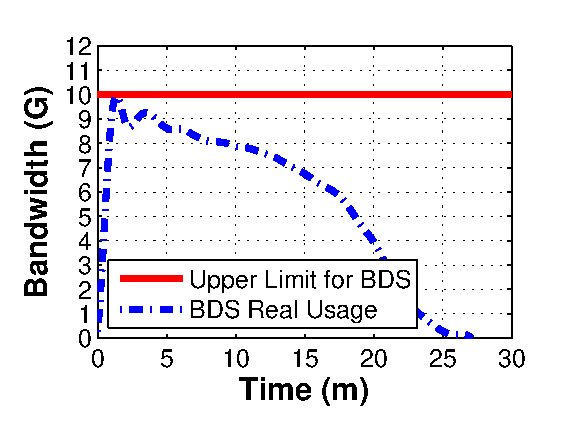
\includegraphics[width=45mm]{images/Quota.eps}
  \tightcaption{The effectiveness of bandwidth separation.}
  \label{fig:quota}
\vspace{-0.4cm}
\end{figure}

To test the effectiveness of bandwidth separation and check whether the bulk data transfers affect latency-sensitive traffic, we set the upper bound of available bandwidth for bulk data transfer to 10~GBs, and monitor the real usage of one inter-DC link. The results are shown in Figure \ref{fig:quota}, from which we can see the real bandwidth usage stays below 10~GBs throughout the whole transmission process.
When being used online, the upper bound of bandwidth for bulk data transfers is set to be the difference between link capacity and the peak bandwidth of latency-sensitive workloads. Therefore, the effectiveness of \name bandwidth separation can guarantee that bulk transfers do not interfere with latency-sensitive workloads.% bound the bunk data transfer, the latency-sensitive workloads would generally not be interfered.
%and thus \name can effectively reduce the incidents of delay on latency-sensitive traffic caused by bulk data transfers.

\begin{table}[t]
\begin{center}
\resizebox{3in}{!}{%
%\begin{tabular}{p{2cm}<{\centering}|p{2cm}<{\centering}}
\begin{tabular}{| c | c | c | c | c |}
\hline
 \rowcolor[gray]{0.9}
\textbf{System} & \textbf{Source DC egress link} & \textbf{$l_1$} & \textbf{$l_2$} & \textbf{$l_3$}\\
\hline \hline
\company & 69.82\% & 53.09\% & 57.98\% & 63.01\% \\
\hline
\name & 70.55\% & 62.46\% & 63.23\% & 64.24\% \\
\hline
\end{tabular}
}
\end{center}
\tightcaption{Average link utilizations of the source DC egress link and 3 inter-DC links ($l_1$, $l_2$, $l_3$) under \company and \name.}
\label{table:usage}
\vspace{-0.4cm}
\end{table}

\begin{figure*}[t]
        \centering
        \begin{subfigure}[b]{0.3\textwidth}
                \centering
                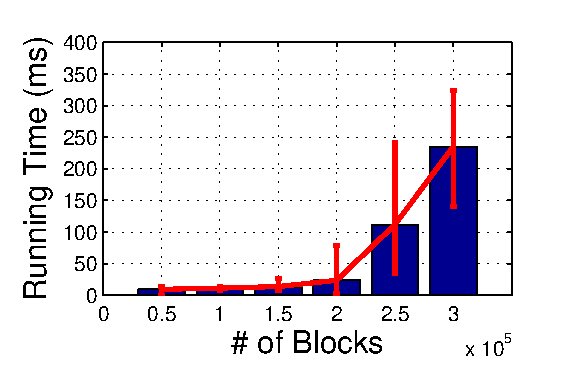
\includegraphics[width=50mm]{images/CPUvsBlk_v2.eps}% cpu.m
                \caption{The controller running time.}
                \label{fig:scale:cpu}
        \end{subfigure}
        \begin{subfigure}[b]{0.3\textwidth}
                \centering
                \includegraphics[width=50mm]{images/NetworkDelay.eps}%CDFofNetworkDelay -> Communication.m
                \caption{The inter-DC network delay.}
                \label{fig:scale:network}
        \end{subfigure}
        \begin{subfigure}[b]{0.3\textwidth}
                \centering
                \includegraphics[width=50mm]{images/CDFofFeedbackLoopDelay.eps}
                \caption{Feedback loop delay.}
                \label{fig:scale:feedback}
        \end{subfigure}
        \tightcaption{[System scalability] Measurements on (a) controller running time, (b) network delay, (c) Feedback loop delay.}
        \label{fig:scale}
\vspace{-0.4cm}
\end{figure*}

\begin{figure*}[t]
        \centering
        \begin{subfigure}[b]{0.3\textwidth}
                \centering
                \includegraphics[width=50mm]{images/failure_v2.eps}%fail.m
                \caption{Average number of downloaded blocks per cycle under failures.}
                \label{fig:analysis:failure}
        \end{subfigure}
        \begin{subfigure}[b]{0.3\textwidth}
                \centering
                \includegraphics[width=50mm]{images/blkSize_v2.eps} %plotTCT_IDC.m
                \caption{Completion time under different block sizes.}
                \label{fig:analysis:blksize}
        \end{subfigure}
        \begin{subfigure}[b]{0.3\textwidth}
                \centering
                \includegraphics[width=50mm]{images/cycleDiff.eps}%cycleDiff.m
                \caption{Completion time under different cycle lengths.}
                \label{fig:analysis:cycleDiff}
        \end{subfigure}
%        \begin{subfigure}[b]{0.3\textwidth}
%                \centering
%                \includegraphics[width=50mm]{images/cycle.eps} %calculation_origin
%                \caption{Reduction on algorithm running time due to approximation.}
%                \label{fig:analysis:time}
%        \end{subfigure}
%        \begin{subfigure}[b]{0.3\textwidth}
%                \centering
%                \includegraphics[width=50mm]{images/overlay.eps}
%                \caption{The proportion of blocks downloaded from the original source.}
%                \label{fig:analysis:overlay}
%        \end{subfigure}
        \tightcaption{\name's (a) fault tolerance, (b) sensitivity to different block sizes, and (c) different cycle lengths.}
        \label{fig:analysis}
\vspace{-0.4cm}
\end{figure*}


As \name implements strict bandwidth separation between latency-sensitive traffic and bulk data transfers while still showing shorter completion time, does it occupy too much bandwidth on inter-DC links? To answer this question, we record the average utilizations of the egress link of the source DC and 3 randomly selected inter-DC links, denoted as $l_1,l_2$ and $l_3$. The result in Table \ref{table:usage} shows that link utilizations do not change much with \name. This is because \name spreads data transfers over bottleneck-disjoint paths, so it avoids transferring the same data on the same link.

%\begin{itemize}
%\item Draw a graph (what graph can you get on this?) to show with bandwidth separation, \name can reduce the incidents of delay on latency-sensitive traffic caused by bulk data transfers.%DrawLink.m
%\item Draw a graph (what graph can you get on this?) to show the link utilization does not change much with \name or with \company.%DrawUsage.m
%\end{itemize}

\subsection{Micro-benchmarks}
\label{subsec:evaluation:benchmarks}

This section examines \name in very details through micro-benchmarks.
%focuses on some benchmarks of \name.
(1) Scalability of the centralized control.
%As \name adopts centralized control, the running time and scalability of the controller are key indicators of algorithm efficiency.
(2) Fault tolerance.
%Algorithm adaptability. \name runs together with latency-sensitive traffic, so high fault tolerance and strong robustness are essential requirements especially in rapidly changing networks. (3). In-depth analysis. The near-optimality of \name and the effects of exploring overlay networks also need to be clarified.
(3) Setting of \name parameters.

\tightsubsubsection{Scalability}\label{subsec:evaluation:benchmarks:scalability}

\mypara{Controller running time} As the controller needs to assign specific transmissions for all blocks, the algorithm running time is naturally related to the number of blocks. We show the relationship of block number and algorithm running time in Figure \ref{fig:scale:cpu}, from which we can see that the controller running time is still lower than $300ms$ even when there are $3\times 10^5$ blocks \myfootnote{$3\times 10^5$ is the instantaneous peak value of block number for a particular large scale CDN service, and $300ms$ is quite reasonable for practical usage.}. This is the instantaneous peak value of block number when the bulk data size is 10~TB, and the block merging scheme described in \Section\ref{subsec:system:centralized} will further reduce the block number and reduce the algorithm running time.

\mypara{Network delay} \name works in inter-DC networks, so the network delay among DCs is a key factor in the algorithm updating process. We record the network delay of 5000 requests and present the CDF in Figure \ref{fig:scale:network}. We can see that 90\% of the network delays are below $50ms$ and the average value is about $25ms$, which is less than 1\% of the decision updating cycle (3 seconds).

\mypara{Feedback loop delay} For centralized algorithms, a small feedback loop delay is essential to algorithm scalability. In \name, this feedback loop consists of several procedures: status updating from agents to the controller, running of the centralized algorithm, and decision updating from the controller back to agents. We measure the delay of the whole process, show the CDF in Figure \ref{fig:scale:feedback}, and find that in most cases (over 80\%), the feedback loop delay is lower than $200ms$. So we can claim that \name demonstrates a short enough update delay and is able to scale to even larger systems.

\begin{figure*}[t]
        \centering
        \begin{subfigure}[b]{0.3\textwidth}
                \centering
                \includegraphics[width=50mm]{images/BDSvsLP_v2.eps} % BDSvsLP.m
                \caption{The reduction on algorithm running time of \name over standard LP.}
                \label{fig:further:BDSvsLP}
        \end{subfigure}
        \begin{subfigure}[b]{0.3\textwidth}
                \centering
                \includegraphics[width=50mm]{images/BDSvsLP_CT.eps}%BDSvsLP_CT -> Communication.m
                \caption{The near-optimality of \name to standard LP in small scale.}
                \label{fig:further:BDSvsLP_CT}
        \end{subfigure}
        \begin{subfigure}[b]{0.3\textwidth}
                \centering
                \includegraphics[width=50mm]{images/overlay.eps}
                \caption{The proportion of blocks downloaded from the original source.}
                \label{fig:further:overlay}
        \end{subfigure}
        \tightcaption{[In-depth analysis] on (a) reduction on algorithm running time, (b) near-optimality, and (c) effects of overlay transmission.}
        \label{fig:further}
\vspace{-0.4cm}
\end{figure*}

%\tightsubsubsection{Algorithm adaptability.}\label{subsubsec:evaluation:adaptability}
\tightsubsubsection{Fault tolerance}

%\mypara{Fault tolerance}
Here we examine the impact of the following failure scenario on the number of downloaded blocks per cycle. During cycles 0 to 9, \name works as usual, and one agent fails in the 10th cycle. The controller fails in the 20th cycle and recovers in the 30th cycle. Figure \ref{fig:analysis:failure} shows the average number of downloaded blocks per cycle. We find that the slight impact of agent failure only lasts for one cycle, and the system recovers in the 11th cycle. When the controller is unavailable, \name falls back to a default decentralized overlay protocol, resulting in graceful performance degradation. With the recovery of the controller, the performance recovers in the 30th cycle.

\tightsubsubsection{Choosing the values of key parameters}\label{subsec:evaluation:benchmarks:parameters}

\mypara{Block size} In \name, the bulk data file is split into blocks and can be transferred on bottleneck-disjoint paths. But this introduces a tradeoff between scheduling efficiency and calculation overhead. We therefore conduct two series of experiments using different block sizes (2MB and 64MB). Figure \ref{fig:analysis:blksize} shows that the completion time in the 2MB/block scenario is 1.5 to 2 times shorter than that in the 64MB/block scenario. This is because a smaller block sizes result in closer-to-optimal performance (see Appendix for the proof). However, this optimization introduces longer controller running time, as shown in Figure \ref{fig:scale:cpu}. We pick block size by balancing two considerations: (1) requirements on the completion time, and (2) controller's operation overhead.

\mypara{Update cycle lengths} Since any change in network environment may potentially alter the optimal overlay routing decisions, \name reacts to the changing network conditions by adjusting the routing scheme periodically. To testify the adjustment frequency, we set different cycle lengths from $0.5s$ to $95s$ to the same bulk data transfer, and Figure \ref{fig:analysis:cycleDiff} shows the completion time. Smaller cycle lengths result in shorter completion time, but the benefit diminishes when the cycle length is less than $3s$. This is because too frequent updates introduce more overhead on: (1) the information collection from agents to the controller, (2) the execution of the centralized algorithm, and (3) the re-establishment of new TCP connection. Thus, considering adjustment granularity and the corresponding overhead, we finally choose $3s$ as the default cycle length.


\tightsubsubsection{In-depth analysis.}\label{subsubsec:evaluation:depth}

\mypara{Optimization over algorithm running time} \name decouples scheduling and routing, which can significantly reduce the computational complexity. To clearly show the optimization, we measure the algorithm running time under \name and the standard linear programming (LP) solution. For the standard LP experiments, we use the \textit{linprog} library on MATLAB \cite{mathworks}, set the upper bound of the iteration number ($10^6$) if the algorithm does not converge, and record the CPU time as a function of the block number. Figure \ref{fig:further:BDSvsLP} shows that the running time of \name keeps below $25ms$ while that of standard LP grows quickly to $4s$ with only 4000 blocks. %This result illustrates \name's optimization over algorithm running time.
\name is much faster than off-the-shelf LP solver.

\mypara{Near-optimality of \name} To measure the near-optimality, we evaluate the data transfer completion time under the standard LP and \name: 2 DCs, 4 servers, 20MBs for server upload/download rate.
%1 to 4000 blocks (we cannot conduct large-scale experiments due to the explosive growth of the LP calculation time).
We vary the number of blocks from 1 to 4000, over which the LP solver can't finish in reasonable time. Figure \ref{fig:further:BDSvsLP_CT} shows that the difference of completion time between \name and the optimal standard LP is about 15\%.


\mypara{Benefit of disjoint overlay paths} \Section\ref{subsec:motivation:case-for} reveals the benefits of disjoint paths on application-level overlay networks. To explore the potential benefit, we record the ratio of the number of blocks downloaded from the original source to the total number of blocks, and the CDF is shown in Figure \ref{fig:further:overlay}. For about 90\% servers, the proportion is less than 20\%, which means that more than 80\% blocks are downloaded from other DCs on the disjoint paths, demonstrating great potential of multicast overlay network.

%\mypara{Breakdown of feedback loop delay} \name also applies the approximation of separating data scheduling from overlay routing, which can also reduce algorithm running time. We show the measurements on algorithm running time in Figure \ref{fig:analysis:time}. At the very beginning, the running time is nearly $800ms$, but drops to $300ms$ and even less quickly. This is because the separated scheduling stage selects only a subset of blocks, making the number of blocks decrease significantly and simplifying the routing decision making process.


%\begin{figure*}[t]
%        \centering
%        \begin{subfigure}[b]{0.3\textwidth}
%                \centering
%                \includegraphics[width=50mm]{images/BDSvsLP.eps} % BDSvsLP.m
%                \caption{Algorithm running time of \name and standard LP.}
%                \label{fig:further:BDSvsLP}
%        \end{subfigure}
%        \begin{subfigure}[b]{0.3\textwidth}
%                \centering
%                \includegraphics[width=50mm]{images/cycleDiff.eps}%cycleDiff.m
%                \caption{Completion time under different cycle lengths.}
%                \label{fig:further:cycleDiff}
%        \end{subfigure}
%        \begin{subfigure}[b]{0.3\textwidth}
%                \centering
%                \includegraphics[width=50mm]{images/failure.eps}%fail.m
%                \caption{Average number of downloaded blocks per cycle under failures.}
%                \label{fig:further:failure}
%        \end{subfigure}
%        \caption{Further analysis on (1) running time, (2) cycle length, and (3) fault tolerance.}
%        \label{fig:further}
%\vspace{-0.4cm}
%\end{figure*}



In summary, both the prototype pilot deployment and the trace-driven simulations of \name show 3-5$\times$ speedup over existing solutions, with good scalability and reliability, and near-optimal scheduling results.


%\begin{itemize}
%\item Scalability of centralized control:
%\begin{itemize}
%\item Y: Bandwidth consumption, vs. X: \# of objects
%\item Y: Controller CPU usage, vs. X: \# of objects
%\item Y: Update delay vs. X: \# of objects
%\item Bar-chart to decompose update delay into collecting updates, running algorithm, and updating local agents
%\end{itemize}
%
%\item In-depth analysis:
%\begin{itemize}
%\item A graph to show the tradeoff caused by different update cycles (why 3 seconds is a good tradeoff?)
%\item Reduction on algorithm running time due to the approximation algorithm.
%\item Maybe another graph from the current 6.3?
%\end{itemize}
%
%\item Fault tolerance:
%\begin{itemize}
%\item Y: flow completion time, vs. X: time. Create a toy topology to send objects. The experiment begins with no failure. At time t1, one server is not available, and the graph should show Y only has performance degradation for less than 3 seconds; At time t2, the controller is not available, and the local agent should automatically revert to decentralized local control.
%\end{itemize}
%
%\end{itemize}





%
\section{Related Work}

%\begin{table*}[t]
%\begin{center}
%\resizebox{\textwidth}{!}{
%\begin{tabular}{| c | c| c |c | c | c |c |}
%\hline
% \rowcolor[gray]{0.9}
%\textbf{Solutions} & \textbf{Design Goal} & \textbf{Network Structure} & \textbf{Data source} & \textbf{Global Info} & \textbf{Control} & \textbf{Hardware Modification} \\
%\hline
%\hline
%B4 \cite{jain2013b4}  & \multirow{2}{*}{Traffic engineering} & \multirow{2}{*}{Non-tiered} & \multirow{2}{*}{Determined} & \multirow{2}{*}{Yes} & \multirow{2}{*}{Software-defined}   & \multirow{2}{*}{Yes}\\
%SWAN \cite{mckeown2009software} &  &  &  &  &  & \\
%\hline
%CDN \cite{kostic2003bullet} & Spread strategy & Tiered & Determined & Yes & Centralized & No \\
%\hline
%%\multirow{2}{*}{Multicast} & No & \multirow{2}{*}{Complete} & \multirow{2}{*}{No} & \multirow{2}{*}{-} & \multirow{2}{*}{Yes}\\
%% & No & & & & \\
%%\hline
%P2P & Data sharing & Non-tiered & Undetermined & No & Distributed & No \\
%\hline
%\hline
%\textbf{\name} & Data distribution & Non-tiered & Undetermined & Yes & Centralized & No\\
%\hline
%\end{tabular}
%}
%\end{center}
%%\vspace{0.1in}
%\vspace{-0.4cm}
%\caption{ Summary of prior works. Data source means when choosing a sender, whether the sender is determined. For undetermined situations, one optimal sender is chosen from multiple candidate senders.}
%\label{table:summary}
%\end{table*}

%Efficient data distribution for IDCs is a hot research topic. Table \ref{table:summary} shows the prior works related with the data distribution problem in our paper.

Here we discuss some representative work that is related to \name in three categories.

\textbf{Overlay Network Control.}
Overlay network releases great potential to various applications, especially for data transfer applications. The representative networks include Peer-to-Peer (P2P) network and Content Delivery Network (CDN). As a mature distributed application protocol, P2P has already been verified by many applications, such as live streaming systems (CoolStreaming \cite{zhang2005coolstreaming}, Joost \cite{Joost}, PPStream \cite{PPStream}, UUSee \cite{UUSee}), video-on-demand (VoD) applications (OceanStore \cite{oceanstore}), distributed hash tables \cite{rhea2005opendht} and even nowaday's Bitcoin \cite{eyal2016bitcoin}, but it cannot achieve the optimal solution due to the lack of global visibility. CDN distributes services spatially relative to end-users to provide high availability and performance (e.g., to reduce page load time), serving many applications such as multimedia \cite{zhu2011multimedia} and live streaming \cite{sripanidkulchai2004analysis}, but the embedded data spread strategies are limited by the layered structure \cite{kostic2003bullet}. \name, is therefore designed in overlay networks with centralized control.

\textbf{Data Transfer and Rate Control.}
Rate control of transport protocols in DC-level plays an important role on data transmissions. DCTCP \cite{Alizadeh2010Data}, PDQ \cite{Hong2012Finishing}, CONGA \cite{Alizadeh2014CONGA}, DCQCN \cite{Zhu2015Congestion} and TIMELY \cite{Mittal2015TIMELY} are all classical protocols showing obvious improvements on transmission efficiency. Besides, some congestion control protocols like the credit-based ExpressPass \cite{Han2017Credit} and load balancing protocols like Hermes \cite{Zhang2017Resilient} could further reduce flow completion time by making rate control. On this basis, the recent proposed Numfabric \cite{nagaraj2016numfabric} and Domino \cite{sivaraman2016packet} further explore the potential of centralized TCP on speeding up data transfer and improving DC throughput. To some extend, co-flow scheduling \cite{Chowdhury2012Coflow,Zhang2016CODA} is a little bit similar to the multicast overlay scheduling, in terms of data parallelism. But they focus on flow-level problems while \name is designed on application-level.% \name is therefore designed in a centralized decision-making manner to approximate the optimal scheduling solution.

\textbf{Centralized Traffic Engineering.} Traffic engineering (TE) has long been a hot research topic, and many existing studies \cite{chen2012design, kavulya2010analysis, mishra2010towards, reiss2012heterogeneity, sharma2011modeling, More, zhang2011characterizing} have illustrated the challenges of scalability, heterogeneity etc., especially on inter-DC level. The representative TE systems include Google's B4 \cite{jain2013b4} and Microsoft's SWAN \cite{hong2013achieving}. B4 adopts SDN \cite{mckeown2009software} and OpenFlow \cite{OpenFlow,mckeown2008openflow} to manage individual switches and deploy customized strategies on the paths. SWAN is another online traffic engineering platform, which achieves high network utilization with its software-driven WAN. %These pair-wise solutions have substantially improved inter-DC WANs, but in inter-DC multicast overlay networks, \name is still essential.% because it can optimally schedule and route data via overlay paths of DC servers.

Overall, an application-level multicast overlay network is essential to data transfer in inter-DC WANs. Applications like user logs, search engine indexes and databases would benefit much from bulk-data multicast. Furthermore, such benefits are orthogonal to prior WAN optimizations, further improving inter-DC applications' performance.
%A pilot deployment of \name, which is in a near-optimal overlay solution over inter-DC WANs for bulk data multicast, has been deployed and evaluated in \company, achieving 3-5$\times$ speedup over the existing system and several widely used overlay routing systems.

%\textbf{Inter-DC management.} Many recent studies \cite{chen2012design, kavulya2010analysis, mishra2010towards, reiss2012heterogeneity, sharma2011modeling, More, zhang2011characterizing} have illustrated the challenges of scalability, heterogeneity and other difficulties. Under these difficulties, some companies published their inter-DC management system, for example Google's B4 \cite{jain2013b4} and Microsoft's SWAN \cite{hong2013achieving}. B4 adopts SDN \cite{mckeown2009software} and OpenFlow \cite{OpenFlow,mckeown2008openflow} to manage individual switch and deploy efficient strategies on the path. SWAN is another online traffic engineering platform, which achieves high network utilization with its software-driven WAN. But these systems can not be applied in our data distribution problem, because: 1) B4, SWAN run on their private self-control backbone networks, both of them are able to manage the links, switches and routers in a software defined manner. However, most of companies do not have the ability, such as \company, the inter-DC links are rent from Internet Service Providers (ISP) and out of self-control. Thus, all the SDN-based solutions become impractical. 2) The design goals are different. B4 and SWAN is aimed to solve the traffic engineering problem. For a particular transmission, data sources and destinations are determined, so the algorithms only need to schedule flows and make routing decisions on the links. But in our data distribution problem, data sources and destinations are undetermined. In summary, these inter-DC management platforms are impractical in our scenario.
%
%\textbf{Content Delivery Network (CDN).} The goal of CDN is to distribute services spatially relative to end-users to provide high availability and performance (e.g., to reduce page load time). Few solutions \cite{kostic2003bullet} focus on data transmission, duplicating data from origin server to servers close to users. They are limited to the tiered structure, i.e., from origin server to edge servers, and then to end servers . But in our data distribution problem, all servers can be treated as in the same tier, and this makes the data transmission more efficient and flexible.
%
%\textbf{P2P-based Schemes.} As a mature distributed application protocol, P2P has already been verified by many applications, such as live streaming systems (CoolStreaming \cite{zhang2005coolstreaming}, Joost \cite{Joost}, PPStream \cite{PPStream}, UUSee \cite{UUSee}), video-on-demand (VoD) applications (OceanStore \cite{oceanstore}), distributed hash tables \cite{rhea2005opendht} and even nowaday's Bitcoin \cite{eyal2016bitcoin}. But P2P does work in the data distribution problem because the lack of global visibility. With the only local information, P2P surely can not make optimal scheduling.


%\ifCLASSOPTIONcompsoc
%  % The Computer Society usually uses the plural form
%  \section*{Acknowledgments}
%\else
%  % regular IEEE prefers the singular form
%  \section*{Acknowledgment}
%\fi
%
%
%The authors would like to thank...
%\small
%\clearpage

%\section{Discussion}

%\section{Conclusion}
\section{Conclusion}
Inter-DC multicast is critical to the performance of
global-scale online service providers, but
prior efforts that focus
on optimizing WAN performance are insufficient.
This paper presents \name,
an application-level multicast overlay network that substantially
improves the performance of
inter-DC bulk-data multicast.
%This paper presents \name, which
\name demonstrates the feasibility
and practical benefits of a fully centralized multicast overlay
network that selects overlay paths and schedules data transfers
in a near-optimal, yet efficient manner.
The key insight underlying \name's centralized design is
that there are significant benefits achieved by making slightly delayed
decisions based on a global view and that this outweighs the cost of
centralization. %, such as gathering information to the controller.
We believe that the insight of decoupling scheduling and routing, to
speed up the execution of a centralized algorithm
%informs our design choice
can be generalized to inspire other centralized control platforms
%in other settings
where centralized decision-making strikes
a favorable balance between costs and benefits.



\bibliographystyle{acm}
\bibliography{DTplatbib}


\section{Appendix}

\textbf{Proof 1: $t_2 > t_1$:}

According to the duplication situations, we classify the $m$ DCs into two sets:

$N_a = \{DC_i|DC_i \text{ has already downloaded block $a$}\}$

$N'_a = \{DC_i|DC_i \text{ hasn't downloaded block $a$}\}$

where $|N_a| + |N'_a| = 2m$. In case 1, all the $n$ blocks has $k$ duplicates, so $|N_i| = k$ and $|N'_i| = 2m-k$. These $2m-k$ transmissions have $k$ optional data sources to download this block. Let $R_{up}$/$R_{down}$ denotes the upload/download rate limit of each server, we can calculate $t_1$ by Equation \ref{caseK}:

\begin{equation}
\label{caseK}
t_1 = \frac{\mathbb{S}}{min\{c(l),\frac{R_{up}\times k}{2m-k},R_{down}\}}
\end{equation}
where $\mathbb{S}$ denotes the size of the remaining data, and $c(l) > R_{up}/2m$ (server upload bandwidth is the bottleneck). This equation is a monotonically decreasing function of $k$ according to the following calculus.

\begin{equation}
\label{calculus}
\begin{split}
t'(k) &= \frac{d(t(k))}{d(k)} = \frac{d(\frac{\mathbb{S}\times (2m-k)}{R_{up}\times k})}{d(k)} \\
    &= \frac{d(\frac{2m\times \mathbb{S}}{R_{up}\times k})}{d(k)} = -\frac{2m\mathbb{S}}{R_{up}\times k^2} \\
    &< 0
\end{split}
\end{equation}

Therefore, in case 2, for those blocks with $k1$ ($k1<k$) duplicates, the completion time $t_{k1}$ will be larger than $t_1$, i.e., $t_2 \geq t_{k1} > t_1$.

\textbf{Proof 2: Near Optimality of \name}

Here we present the proof of rounding the integer solution.

\name distributes each task in an optimal manner given by the maximum concurrent flow (MCF) solution \cite{reed2012traffic}. However, the MCF solution is a linear relaxation of the original integer problem and in practice the solution requires that flows are routed as integers of the block size flow. There are a number of strategies using the output of the MCF for the integer path allocation, however, none of them will be strictly optimal as the original problem is NP-complete. A common strategy is to use \emph{randomized-rounding}. Randomized-rounding was first analyzed in detail for some relaxation approaches by Raghavan and Thompson \cite{Raghavan1987} and a similar approach is followed here for the specific case of the MCF relaxation for which they do not provide a solution. A flow through an arbitrary edge, \(e\) is denoted, as \(f_e=\sum_{e \in p_\lambda} F_{B_{i,j},p_\lambda} \; \forall \; p_\lambda\) where $F^*$ is the optimum value in the MCF problem that is equivalent to $f^*$ in the original problem. $f_e$ is the optimal MCF flow through edge $e$ that in the integer solution is approximated from the flow of multiple blocks each of flow rate $b$. To perform the randomized rounding, first, each of the \emph{fractional flows}  $F_{B_{i,j},p_\lambda}$ is truncated to an \emph{integer flow} that is constructed from a number of\emph{ block flows}, each integer flow is denoted as $\left \lfloor F_{B_{i,j},p_\lambda} \right \rfloor = kb \leq F_{B_{i,j},p_\lambda}$ where $k$ is strictly the largest positive integer, or zero, to meet the constraint. Then each integer flow is either kept at $kb$ or \emph{rounded} up with probability $(F_{B_{i,j},p_\lambda} - \left \lfloor{F_{B_{i,j},p_\lambda}} \right \rfloor)/b$ to $(k+1)b$. This rounding probability means that the expected value of the integer flows is $f_e$, the solution of the optimal linear MFC. The problem is then to determine the likelihood that this rounding will cause the capacity constraint on an edge $e$ to be exceeded. To aid the discussion, a \emph{residual flow}  $f^\prime_e=f_e - \sum_{e \in p_\lambda} \left \lfloor{F_{B_{i,j},p_\lambda}} \right \rfloor $ is used to describe the flow that needs to be added to the truncated flows to obtain the optimal solution obtained from MFC.

As each flow rounding is an independent random variable, we can determine the likelihood of exceeding the capacity constraint by applying the following well-known Chernoff bound~\cite{chernoff1952}:
\begin{equation}
  \label{chernoff}
  \Pr(X > (1+\delta)\mu) \leq e^{\frac{2\delta^2\mu^2}{n(b-a)^2}}
\end{equation}
where $X=X_1 + \ldots X_n$ is the sum of independent, bounded, random variables $a \leq X_i \leq b$ and $\mu = E{(X)} $. This bound describes the probability that a summation of random variables exceeds the expected value of the sum by a factor of $\delta$. In the problem considered here, the random variables are the rounded flows which have an expected summation $\mu = f^\prime_e$. Consider an edge, $e$, that has its capacity fully used by the linear MFC solution. Using the Chernoff bound from Equation~\eqref{chernoff}, note that $a=0$ and the highest value of the rounded flow added is one block with flow $b$ then we find that the factor that the integer flow is beyond optimal, and the residual flow is bounded by:
\begin{equation}
  \label{block}
  \delta \leq \frac{b}{r} \sqrt{\frac{n}{2}\ln\epsilon}
\end{equation}
with probability $1-\epsilon$. It should be noted that as the size of the blocks becomes small compared to the overall flow $f_e$, the probability that the linear flow is exceeded by a factor $\delta$ becomes exponentially small due to the exponential form of the Chernoff bound.


\end{document}
